% file: Gravity_Notes_grande.tex
% Me, working out the lectures, examples, and homework for the BEST VIDEO LECTURE SERIES on General Relativity and Gravity, ever:
% WE Heraeus International Winter School on Gravity and Light
%
% MIT OCW (Massachusetts Institute of Technology Open CourseWare) for 8.962 Fall 2006, Kamiokowski's website, and various other places
% 
% If you liked this this file or found it useful, please consider donating on my Tilt/Open 
% campaign: I'd want to raise money for a new computer. 
% ernestyalumni.tilt.com 
%
% Facebook      : ernestyalumni 
% github        : ernestyalumni
% gmail         : ernestyalumni 
% linkedin      : ernestyalumni 
% twitter       : ernestyalumni 
% wordpress.com : ernestyalumni
% youtube       : ernestyalumni 
% Tilt/Open     : ernestyalumni
%
% This code is open-source, governed by the Creative Common license.  Use of this code is governed by the Caltech Honor Code: ``No member of the Caltech community shall take unfair advantage of any other member of the Caltech community.'' 
% 

\documentclass[10pt, twoside]{amsart}
\pdfoutput=1
\usepackage{mathtools,amssymb,lipsum,caption}

\setcounter{tocdepth}{1} % to get subsubsections in toc 
% cf. http://www.latex-community.org/forum/viewtopic.php?f=47&p=44760


\usepackage{graphicx}
\usepackage{hyperref}
\usepackage[utf8]{inputenc}

\usepackage{cancel} % http://jansoehlke.com/2010/06/strikethrough-in-latex/
\usepackage{listings}
\usepackage[table]{xcolor}
\usepackage{pdfpages}
\usepackage{tikz}
\usetikzlibrary{matrix,arrows,calc,decorations.pathmorphing,shapes}

\usepackage{pifont} % http://tug.ctan.org/info/symbols/comprehensive/symbols-a4.pdf

\usepackage{multicol}

\hypersetup{colorlinks=true,citecolor=[rgb]{0,0.4,0}}

\oddsidemargin=15pt
\evensidemargin=5pt
\hoffset-45pt
\voffset-55pt
\topmargin=-4pt
\headsep=5pt
\textwidth=1120pt
\textheight=595pt
\paperwidth=1200pt
\paperheight=700pt
\footskip=40pt







\newtheorem{axiom}{Axiom}
\newtheorem{theorem}{Theorem}
\newtheorem{corollary}{Corollary}
%\newtheorem*{main}{Main Theorem}
\newtheorem{lemma}{Lemma}
\newtheorem{proposition}{Proposition}

\newtheorem{definition}{Definition}
\newtheorem{remark}{Remark}

\newenvironment{claim}[1]{\par\noindent\underline{Claim:}\space#1}{}
\newenvironment{claimproof}[1]{\par\noindent\underline{Proof:}\space#1}{\hfill $\blacksquare$}

%This defines a new command \questionhead which takes one argument and
%prints out Question #. with some space.
\newcommand{\questionhead}[1]
  {\bigskip\bigskip
   \noindent{\small\bf Question #1.}
   \bigskip}

\newcommand{\problemhead}[1]
  {
   \noindent{\small\bf Problem #1.}
   }

\newcommand{\exercisehead}[1]
  { \smallskip
   \noindent{\small\bf Exercise #1.}
  }

\newcommand{\solutionhead}[1]
  {
   \noindent{\small\bf Solution #1.}
   }


%-----------------------------------
\begin{document}

%-----------------------------------

\title[GR]{Notes on General Relativity (GR) and Gravity}
\author{Ernest Yeung}
\address{}
\email{ernestyalumni@gmail.com}
\urladdr{http://ernestyalumni.wordpress.com ernestyalumni.tilt.com }
\thanks{I write notes, review papers, and code and make calculations for physics, math, and engineering to help with education and research. With your support, we can keep education and research material available online, openly accessible, and free for anyone, anytime. If you like what I'm trying to do for physics education research, please go to my Tilt/Open crowdfunding campaign, read the mission statement, share the page, and contribute financially if you can. ernestyalumni.tilt.com }
\keywords{General Relativity, Gravity, Differential Geometry, Manifolds, Integration, MIT OCW, education, mathematics, physics}
\subjclass[GR]{General Relativity}
\date{23 mars 2015}
\begin{abstract}
These are notes on General Relativity (GR) and Gravity.

As of March 23, 2015, I find that the Central Lectures given by Dr. Frederic P. Schuller for the WE Heraeus International Winter School to be, unequivocally, the best, most lucid, and well-constructed lecture series on General Relativity and Gravity.  Instead of reinventing the wheel, I write these notes to build upon and supplement the video lectures and tutorials already created by them.  This includes my corrections, comments, relations to other aspects of theoretical physics, and code implementing calculations in GR.  

It should be noted that for symbolic computation, I heavily use the SageManifolds v.0.7 package for Sage Math.  My goal in this area is this: we see a concept or idea from GR and we go from the equation on the blackboard or textbook and into (Python/Sage Math) code that immediately computes a calculation.

I keep these notes available online, openly accessible, and free for anyone, anytime (with your (financial) help and contribution at Tilt/Open, which is a subscription service).  I want to keep these notes openly accessible because I want to encourage anyone to freely edit, copy, and make their own notes in the spirit of open-source software.

I continuously update these notes and post them here \url{ernestyalumni.wordpress.com}

The stated goal of the WE Heraeus International Winter School on Gravity and Light is to take the student from an introduction to the research frontier (cf. \url{http://www.gravity-and-light.org/lectures}). I want to get myself and other students or ambitious non-academic (maybe he or she is a working professional who had studied physics before in college, went to work in another field, maybe even, gasp, investment banking or mobile app developer, but still is curious and passionate about physics and want to contribute) equipped with all the tools available to do research, do calculations, to design experiments or collect data. Again, we're not here to reinvent the wheel. I'm not trying to make a General Relativity appreciation class, but this is a serious attempt towards training to do research.  
\end{abstract}

\maketitle


\definecolor{darkgreen}{rgb}{0,0.4,0}
\lstset{language=Python,
 frame=bottomline,
 basicstyle=\scriptsize,
 identifierstyle=\color{blue},
 keywordstyle=\bfseries,
 commentstyle=\color{darkgreen},
 stringstyle=\color{red},
 }
%\lstlistoflistings

\tableofcontents

\begin{multicols*}{2}



\part{WE Heraeus International Winter School on Gravity and Light}

\section*{Introduction (from EY)}

The International Winter School on Gravity and Light held \emph{central lectures} given by Dr. Frederic P. Schuller. These lectures on General Relativity and Gravity are unequivocally and undeniably, the best and most lucid and well-constructed lecture series on General Relativity and Gravity.  The mathematical foundation from topology and differential geometry from which General Relativity arises from is solid, well-selected in rigor.  The lectures themselves are well-thought out and clearly explained.  

Even more so, the International Winter School provided accompanying Tutorial Sessions for each of the lectures.  I had given up hopes in seeing this component of the learning process ever be put online so that anyone and everyone in the world could learn through the Tutorial process as well.  I was afraid that nobody would understand how the Tutorial or ``Office Hours'' session was important for students to digest and comprehend and work out-doing exercises-the material presented in the lectures.  This International Winter School gets it and shows how online education has to be done, to do it in an excellent manner, moving forward.  

For anyone who is serious about learning General Relativity and Gravity, I would simply point to these video lectures and tutorials.  

What I want to do is to build upon the material presented in this International Winter School.  Why it's important to me, and to the students and practicing researchers out there, is that the material presented takes the student from an introduction to the research frontier.  That is the stated goal of the International Winter School.  I want to dig into and help contribute to the cutting edge in research and this entire program with lectures and tutorials appears to be the most direct and sensible route directly to being able to do research in General Relativity and Gravity. -EY 20150323


\section{Lecture 1: Topology}

\subsection{Lecture 1: Topological Spaces}

\begin{definition}
  Let $M$ be a set.  \\
A \textbf{topology} $\mathcal{O}$ is a subset $\mathcal{O} \subseteq \mathcal{P}(M)$, $\mathcal{P}(M)$ power set of $M$: set of all subsets of $M$. satisfying
\begin{enumerate}
  \item[(i)] $\emptyset \in \mathcal{O}$, $M \in \mathcal{O}$ 
\item[(ii)] $ U \in \mathcal{O}$, \, $V \in \mathcal{O} \Longrightarrow U\bigcap V \in \mathcal{O}$ 
\item[(iii)] $U_{\alpha} \in \mathcal{O}$, \, $\alpha \in \mathcal{A}$ \, $\Longrightarrow \left( \bigcup_{\alpha \in \mathcal{A}} U_{\alpha} \right) \in \mathcal{O}$
\end{enumerate}
\end{definition}

$ \left. \mathcal{O} \right\} $ utterly useless

\begin{definition}
  $\mathcal{O}_{\text{standard}} \subseteq \mathcal{P}(\mathbb{R}^d)$
\end{definition}

EY : 20150524 

I'll fill in the proof that $\mathcal{O}_{\text{standard}}$ is a topology.  

\begin{proof}
  $\emptyset \in \mathcal{O}_{\text{standard}}$ \\
since $\forall \, p \in \emptyset$, $\exists \, r \in \mathbb{R}^+$: $\mathcal{B}_r(p) \subseteq \emptyset$ (i.e. satisfied ``vacuously'') \\

Suppose $U,V \in \mathcal{O}_{\text{standard}}$.  \\
Let $p \in U \bigcap V$.  Then $\exists \, r_1, r_2 \in \mathbb{R}^+$ s.t. $\begin{aligned} & \quad \\
  & \mathcal{B}_{r_1}(p) \subseteq U \\
  & \mathcal{B}_{r_2}(p) \subseteq V \end{aligned}$ \\

Let $r=\min{ \lbrace r_1, r_2 \rbrace}$.   \\
Clearly $\mathcal{B}_r(p) \subseteq U$ and $\mathcal{B}_r(p) \subseteq V$.  Then $\mathcal{B}_r(p) \subseteq U \bigcap V$.  So $U\bigcap V \in \mathcal{O}_{\text{standard}}$.   \\

Suppose, $U_{\alpha} \in \mathcal{O}_{\text{standard}}$, $\forall \, \alpha \in \mathcal{A}$.  \\
Let $p \in \bigcup_{\alpha \in \mathcal{A}} U_{\alpha}$.  Then $p \in U_{\alpha}$ for at least 1 $\alpha \in \mathcal{A}$.  \\
\phantom{ \quad \, } $\exists \, r_{\alpha} \in \mathbb{R}^+$ s.t. $\mathcal{B}_{r_{\alpha}}(p) \subseteq U_{\alpha} \subseteq \bigcup_{\alpha \in \mathcal{A}} U_{\alpha}$.  So $\bigcup_{\alpha \in \mathcal{A}} U_{\alpha} \in \mathcal{O}_{\text{standard}}$  
\end{proof}


\subsection{2. Continuous maps}

\subsection{3. Composition of continuous maps}

\subsection{4. Inheriting a topology}


EY : 20150524

I'll fill in the proof that given $f$ continuous (cont.), then the restriction of $f$ onto a subspace $S$ is cont.  If you want a reference, check out Klaus J\"{a}nich \cite[pp. 13, Ch. 1 Fundamental Concepts, Sec. Continuous Maps]{KJanich1995}

If cont. $f: M \to N$, $S \subseteq M$, then $\left. f \right|_S$ cont.  

\begin{proof}
  Let open $V \subseteq N$, i.e. $V \in \mathcal{O}_N$ i.e. $V$ in the topology $\mathcal{O}_N$ of $N$.  
\[
\left. f\right|_S^{-1}(V) = \lbrace m \in M | \left. f \right|_S(m) \in V \rbrace
\]
Now $f^{-1}(V) = \lbrace m \in M | f(m) \in V \rbrace$. \\
So $f^{-1}(V) \bigcap S = \left. f \right|_S^{-1}(V)$

Now $f$ cont. So $f^{-1}(V) \in \mathcal{O}_N$.  \\
and recall $\left. \mathcal{O}_S \right| := \lbrace U \bigcap S | U \in \mathcal{O}_M \rbrace$.  

so $f^{-1}(V) \bigcap S = \left. f \right|_S^{-1}(V) \in \mathcal{O}_S$ i.e. $\left. f\right|_S^{-1}(V)$ open. \\
$\Longrightarrow \left. f\right|_S$ cont.  
\end{proof}

\section*{Topology Tutorial Sheet}
filename : \texttt{main.pdf} \\
The WE-Heraeus International Winter School on Gravity and Light: Topology \\

EY : 20150524  

What I won't do here is retype up the solutions presented in the Tutorial (cf. \url{https://youtu.be/_XkhZQ-hNLs}): the presenter did a very good job.  If someone wants to type up the solutions and copy and paste it onto this LaTeX file, in the spirit of open-source collaboration, I would encourage this effort. 

Instead, what I want to encourage is the use of as much CAS (Computer Algebra System) and symbolic and numerical computation because, first, we're in the 21st century, second, to set the stage for further applications in research.  I use Python and Sage Math alot, mostly because they are open-source software (OSS) and fun to use.  Also note that the structure of Sage Math modules matches closely to Category Theory.  

In checking whether a set is a topology, I found it strange that there wasn't already a function in Sage Math to check each of the axioms.  So I wrote my own; see my code snippet, which you can copy, paste, edit freely in the spirit of OSS here, titled \texttt{topology.sage}: 

\href{https://gist.github.com/ernestyalumni/903eefd01be1f214598b}{gist github ernestyalumni topology.sage} \\
\href{https://gist.githubusercontent.com/ernestyalumni/903eefd01be1f214598b/raw/67083e3b3dec2faf2087713236b413b741bd1180/topology.sage}{Download topology.sage}

Loading \texttt{topology.sage}, after changing into (with the usual Linux terminal commands, cd, ls) by 
\lstset{language=Python,basicstyle=\scriptsize\ttfamily,
    commentstyle=\ttfamily\color{gray}}
\begin{lstlisting}[frame=single]
sage: load(``topology.sage'')
\end{lstlisting}

\exercisehead{2: Topologies on a simple set}

\questionhead{Does $\mathcal{O}_1:= \dots$ constitute a topology \dots?}

\textbf{Solution}: Yes, since we check by typing in the following commands in Sage Math:

\begin{lstlisting}[frame=single]
emptyset in O_1
Axiom2check(O_1) # True
Axiom3check(O_1) # True
\end{lstlisting}

\questionhead{What about $\mathcal{O}_2$ \dots ?}

\textbf{Solution}: No since the 3rd. axiom fails, as can be checked by typing in the following commands in Sage Math:
\begin{lstlisting}[frame=single]
emptyset in O_2
Axiom2check(O_2) # True
Axiom3check(O_2) # False
\end{lstlisting}

\section{Lecture 2: Topological Manifolds}

\subsection*{Lecture 2: Manifolds}

Topological spaces: $\exists \,$ so man that mathematicians cannot even classify them. 

For spacetime physics, we may focus on topological spaces $(M,\mathcal{O})$ that can be \underline{charted}, analogously to how the surface of the earth is charted in an \underline{atlas}.

\subsection{Topological manifolds}

\begin{definition}
  A topological space $(M,\mathcal{O})$ is called a \textbf{$d$-dimensional topological method} if \\
$\forall \, p \in M : \, \exists \, U \in \mathcal{O}, \, U \ni p \, : \, \exists \, x : U \subseteq M \to x(U) \subseteq \mathbb{R}^d$  \quad \quad \, $(M,\mathcal{O}), ( \mathbb{R}^d , \mathcal{O}_{\text{std}})$ 
\begin{enumerate}
  \item[(i)] $x$ \textbf{ invertible }: 
\[
x^{-1}:x(U) \to U
\]
\item[(ii)] $x$ \textbf{ continuous }
\item[(iii)] $x^{-1}$ \textbf{ continuous }
\end{enumerate}
\end{definition}

\subsection{Terminology}

\subsection{3. Chart transition maps}

Imagine 2 charts $(U,x)$ and $(V,y)$ with overlapping regions.  

\subsection{4. Manifold philosophy}

Often it is desirable (or indeed the way) to define properties (``continuity'') of real-world object (``$\mathbb{R}\xrightarrow{ \gamma } M$'') by judging suitable coordinates not on the ``real-world'' object itself, but on a chart-representation of that real world object.  

\subsection*{EY's add-ons}

This lecture gives me a good excuse to review Topology and Topological Manifolds from a mathematician's point of view.  I find John M. Lee's \textbf{Introduction to Topological Manifolds} book good because it's elementary and thorough and it's fairly recent (2010) so it's up to date \cite{JMLee2010}.  See my notes and solutions for the book; it's a file titled \verb|LeeJM_IntroTopManifolds_sol.pdf| of which I'll try to keep the pdf and LaTeX file available for download on my ernestyalumni Google Drive (so try to search for it on Google).  

%20150531 : EY I was going to remark on the reasons why I write up solutions, but they include a very personal (but real) experience and in reflection, this is probably better left on another medium.

%There are 3 reasons that come up to mind why I write up these solutions: 1. I'm trying to learn the material myself and at the very minimum, the learning process at the start is \emph{imitating the master}.  I try to find interesting exercises and problems to work out and if I can't do it, then I try to get help fast (mostly online, and mostly with stackexchange).  2. I'm trying to organize my notes and what I've learned and I've moved so much over the years that having it online or on a hard drive works better than for me to carry notebooks.  I still remember how by my Winter 2012/2013 semester I was furiously typing up my notes on LaTeX to get a handle of organization and it paid off, because when I was robbed and assaulted the second time during my Masters studies, and had to quickly grab all my worldly possessions on my back, both hands, around my neck, through the snow, I was glad I didn't have anymore textbooks or notebooks than I did have (cf. \href{``Facing evil Pt. 1''}{https://medium.com/@ernesttravels/facing-evil-part-1-664bb515c6f5}).  ``When you want to succeed as bad as you want to breathe,\dots'' cf. Eric Thomas.  3. I appreciate that learning math and physics can be dreadfully lonely.  I hope to encourage the study of these fairly difficult subjects, like General Relativity and Topology through these notes and solutions; you're not alone in your struggle!



\section*{Tutorial Topological manifolds}

filename: \verb|Sheet_1.2.pdf|

%\exercisehead{1}

\exercisehead{4: Before the invention of the wheel}

\emph{Another one-dimensional topological manifold. Another one?}

Consider set $F^1:= \lbrace (m,n)\in \mathbb{R}^2 | m^4 + n^4=1 \rbrace$, equipped with subset topology $\left. \mathcal{O}_{\text{std}} \right|_{F^1}$

\questionhead{$x:F^1 \to \mathbb{R}$ is what?}

\solutionhead{} EY : 20150525 The tutorial video \url{https://youtu.be/ghfEQ3u_B6g} is really good and this solution is how I'd write it, but it's really the same (I needed the practice).

\[
\boxed{ \begin{aligned}
   x : F^1 & \to \mathbb{R} \\ 
  (m,n) & \mapsto m
\end{aligned} }
\]

If $m=0$, $n^4=1$ so $n=\pm 1$ so it's not injective.  

Let the closed $n$-dim. upper half-space $\mathbb{H}^n \subseteq \mathbb{R}^1$.  Then
\[
\begin{aligned}
  \mathbb{H}^n = \lbrace (x_1 \dots x_n) \in \mathbb{R}^n | x_n \geq 0 \rbrace \\ 
  \text{int}\mathbb{H}^n = \lbrace (x_1 \dots x_n) \in \mathbb{R}^n | x_n > 0 \rbrace \\
  - \mathbb{H}^n = \lbrace (x_1 \dots x_n) \in \mathbb{R}^n | x_n \leq 0 \rbrace \\ 
  -\text{int}\mathbb{H}^n = \lbrace (x_1 \dots x_n) \in \mathbb{R}^n | x_n <0 \rbrace
\end{aligned}
\]

\questionhead{This map $x$ may be made injective by restricting its domain to either of 2 maximal open subsets of $F^1$. Which ones?}

\solutionhead{}

Let 
\[
\begin{aligned}
  & U_+ = F^1 \cap \text{int}\mathbb{H}^2 \\
  & U_- = F^1 \cap -\text{int}\mathbb{H}^2
\end{aligned}
\]

Look at 
\[
\begin{aligned}
  & x^4 = 1 - n^4 \\ 
  \Longrightarrow & x = \pm ( 1 - n^4)^{1/4}
\end{aligned}
\]

Then for 
\[
\begin{aligned}
  x_+^{-1}: (-1,1) \subseteq \mathbb{R} & \to U_+ \\ 
  m & \mapsto (m,(1-m^4)^{1/4}) \\
  x_-^{-1}: (-1,1) \subseteq \mathbb{R} & \to U_- \\ 
  m & \mapsto (m,-(1-m^4)^{1/4}) \\
\end{aligned}
\]
$x_+$,$x_-$ injective (since left inverse exists).  


\questionhead{Construct injective $y$}

\solutionhead{}

Let 
\[
\begin{aligned}
  & V_+ = F^1 \cap \text{int}\mathbb{H}^1 \\
  & V_- = F^1 \cap -\text{int}\mathbb{H}^1
\end{aligned}
\]

Then
\[
\begin{aligned}
  y_+:  V_+ & \to  (-1,1) \subseteq \mathbb{R} \\ 
  (m,n) & \mapsto n \\
  y_-: V_-  & \to  (-1,1) \subseteq \mathbb{R}  \\ 
  (m,n) & \mapsto n
\end{aligned}
\]

\questionhead{Construct inverse $y^{-1}$}
\solutionhead{}


For 
\[
\begin{aligned}
  y_+^{-1}: (-1,1) \subseteq \mathbb{R} & \to V_+ \\ 
  n & \mapsto ((1-n^4)^{1/4},n) \\
  y_-^{-1}: (-1,1) \subseteq \mathbb{R} & \to V_- \\ 
  n & \mapsto (-(1-n^4)^{1/4},n) \\
\end{aligned}
\]
$y_+$,$y_-$ injective (since left inverse exists).  



Note $\begin{aligned} & \quad \\ 
  & (-1,0) \notin U_+,U_- \\
  & (1,0) \notin U_+,U_- \\
\end{aligned}$

and 

 $\begin{aligned} & \quad \\ 
  & (0,1) \notin V_+,V_- \\
  & (0,-1) \notin V_+,V_- \\
\end{aligned}$


\questionhead{construct \emph{transition map } $x \circ y^{-1}$}

\solutionhead{}

\[
\begin{aligned}
& 
\begin{aligned}
   x_+y_+^{-1} : (0,1) \subseteq \mathbb{R} & \to (0,1) \subseteq \mathbb{R} \\ 
  n & \mapsto (1-n^4)^{1/4} 
\end{aligned}   \\ 
& 
\begin{aligned}
   x_-y_+^{-1} : (-1,0) \subseteq \mathbb{R} & \to (0,1) \subseteq \mathbb{R} \\ 
  n & \xrightarrow{ y_+^{-1} } ( (1-n^4)^{1/4}, n) \xrightarrow{ x_- } (1-n^4)^{1/4} 
\end{aligned}   \\ 
& \begin{aligned}
   x_+y_-^{-1} : (0,1) \subseteq \mathbb{R} & \to (-1,0) \subseteq \mathbb{R} \\ 
  n & \mapsto -(1-n^4)^{1/4} 
\end{aligned}   \\ 
& \begin{aligned}
   x_-y_-^{-1} : (-1,0) \subseteq \mathbb{R} & \to (-1,0) \subseteq \mathbb{R} \\ 
  n & \mapsto -(1-n^4)^{1/4} 
\end{aligned}   
\end{aligned}
\]

\questionhead{\dots Does the collection of these domains and maps form an atlas of $F^1$?}

Yes, with atlas

\[
\mathcal{A} = \lbrace \begin{aligned} & (U_+,x_+) \\
  & (U_-,x_-) \end{aligned}, \, \begin{aligned} & (V_+,y_+) \\ & (V_-,y_-) \end{aligned} \rbrace
\]

Clearly 
\[
\begin{gathered}
  U_+ \cup U_- \cup V_+ \cup V_- = (F^1 \cap \text{int}\mathbb{H}^2) \cup (F^1 \cap -\text{int}\mathbb{H}^2)\cup (F^1 \cap \text{int}\mathbb{H}^1) \cup (F^1 \cap -\text{int}\mathbb{H}^1) = \\
= F^1 \cap \mathbb{R}^2\backslash \lbrace (0,0) \rbrace = F^1
\end{gathered}
\]
and (the point is that) $x_{\pm},y_{\pm}$ are homeomorphisms of open sets of $F^1$ onto open sets of 1 dim. $\mathbb{R}^1$ (namely $(-1,1) \subseteq \mathbb{R}^1$), and so $\mathcal{A}$ is an atlas of $F^1$.  

\section{}

\section{Lecture 4: Differentiable Manifolds}

so far: top. mfd. $\begin{gathered}  \quad \\ 
  (M,\mathcal{O}) \\
  \text{dim}M = d \end{gathered}$

we wish to define a notion of differentiable  \\
\phantom{ \quad \quad \, } curves $\mathbb{R} \to M$ \\
\phantom{ \quad \quad \, } function $M \to \mathbb{R}$ \\
\phantom{ \quad \quad \, } maps $M \to N$

\subsection{1. Strategy}  choose a chart $(U,x)$ 

$\gamma : \mathbb{R} \to M$  portion of curve in chart domain


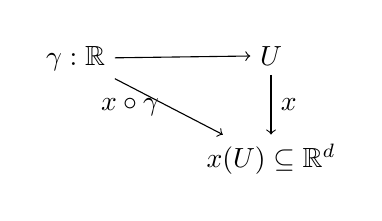
\begin{tikzpicture}[decoration=snake]
  \matrix (m) [matrix of math nodes, row sep=2em, column sep=3em, minimum width=1em]
  {
\gamma : \mathbb{R} & U \\
& x(U) \subseteq \mathbb{R}^d \\ 
};
  \path[->]
  (m-1-1) edge node [above] {$$} (m-1-2)
          edge node [left] {$x\circ \gamma$} (m-2-2)
  (m-1-2) edge node [right] {$x$} (m-2-2);
\end{tikzpicture}
\underline{idea}. try to ``lift'' the undergraduate notion of differentiability of a curve on $\mathbb{R}^d$ to a notion of differentiability of a curve on $M$

\underline{Problem} Can this be well-defined under change of chart?

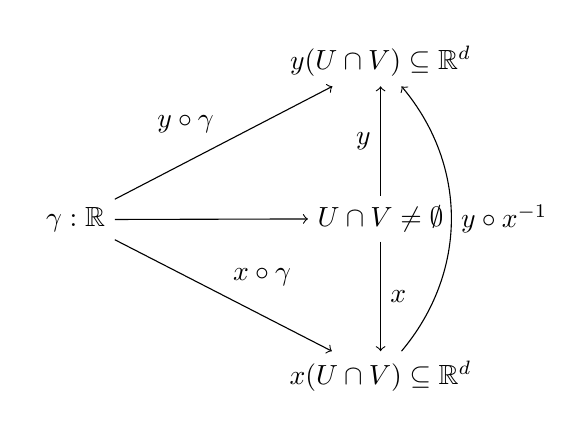
\begin{tikzpicture}[decoration=snake]
  \matrix (m) [matrix of math nodes, row sep=4em, column sep=6em, minimum width=2em]
  {
    & y(U\cap V) \subseteq \mathbb{R}^d \\ 
\gamma : \mathbb{R} & U \cap V \neq \emptyset \\
& x(U\cap V) \subseteq \mathbb{R}^d \\ 
};
  \path[->]
  
  (m-2-1) edge node [auto] {$$} (m-2-2)
          edge node [auto] {$x\circ \gamma$} (m-3-2)
          edge node [auto] {$y\circ \gamma$} (m-1-2)
  (m-2-2) edge node [auto] {$x$} (m-3-2)
          edge node [auto] {$y$} (m-1-2)
  (m-3-2) edge [bend right=40] node [right] {$y\circ x^{-1}$} (m-1-2);
\end{tikzpicture}

$x\circ \gamma$ undergraduate differentiable (``as a map $\mathbb{R} \to \mathbb{R}^d$'')

\[
\begin{gathered}
  \underbrace{y\circ \gamma}_{\text{maybe only continuous, but not undergraduate differentiable} } =  \underbrace{ ( \overbrace{ y\circ x^{-1}}^{\mathbb{R}^d \to \mathbb{R}^d }   )}_{\text{continuous}}  \circ \underbrace{ \overbrace{ (x\circ \gamma) }^{\mathbb{R}\to \mathbb{R}^d} }_{ \text{ undergrad differentiable } }  = y \circ (x^{-1} \circ x) \circ \gamma
\end{gathered}
\]

At first sight, strategy does not work out.  

\subsection{2. Compatible charts}

In section 1, we used any imaginable charts on the top. mfd. $(M,\mathcal{O})$.  

To emphasize this, we may say that we took $U$ and $V$ from the \emph{maximal atlas} $\mathcal{A}$ of $(M,\mathcal{O})$.  


\begin{definition}
Two charts $(U,x)$ and $(V,y)$ of a top. mfd. are called \ding{96}-compatible if 
either
\begin{enumerate}
  \item[(a)] $U \cap V = \emptyset$
or  \item[(b)] $U\cap V \neq \emptyset$
\end{enumerate}
chart transition maps have undergraduate \ding{96} property.

EY : 20151109 e.g. since $\mathbb{R}^d \to \mathbb{R}^d$, can use undergradate \ding{96} property such as continuity or differentiability.

\[
\begin{aligned}
  & y \circ x^{-1} : x(U \cap V) \subseteq \mathbb{R}^d  \to y(U\cap V) \subseteq \mathbb{R}^d  \\
  & x\circ y^{-1} : y(U\cap V) \subseteq \mathbb{R}^d   \to x(U\cap V) \subseteq \mathbb{R}^d
\end{aligned}
\]
\end{definition}

\underline{Philosophy}: 

\begin{definition}
  An atlas $\mathcal{A}_{\text{\ding{96}}}$ is a \ding{96}-compatible atlas if any two charts in $\mathcal{A}_{\text{\ding{96}}}$ are \ding{96}-compatible.

\end{definition}

\begin{definition}
  A \textbf{\ding{96}-manifold} is a triple $(\underbrace{ M,\mathcal{O} }_{\text{top. mfd.} }, \mathcal{A}_{\text{\ding{96}}})$ \quad \, $\mathcal{A}_{\text{\ding{96}}} \subseteq \mathcal{A}_{\text{maximal}} $
\end{definition}


\begin{tabular}{ l | c  l}
\ding{96} &  undergraduate  \ding{96} &  \\
\hline
$C^0$ & $C^0(\mathbb{R}^d \to \mathbb{R}^d) =$  &  continuous maps w.r.t. $\mathcal{O}$  \\
$C^1$ & $C^1(\mathbb{R}^d \to \mathbb{R}^d) = $  &  differentiable (once) and is continuous  \\
$C^k$ & & $k$-times continuously differentiable \\
$D^k$ & & $k$-times differentiable \\
$\vdots$ & & \\
$C^{\infty}$ & $C^{\infty}(\mathbb{R}^d \to \mathbb{R}^d)$ & \\
$\mathbin{\rotatebox[origin=c]{-90}{$\supseteq$}}$ & &  \\
$C^{\omega}$ & $\exists $  multi-dim. Taylor exp.  &  \\
$\mathbb{C}^{\infty}$ & satisfy Cauchy-Riemann equations, pair-wise & 
\end{tabular}


EY : 20151109 Schuller says: $C^k$ is easy to work with because you can judge $k$-times cont. differentiability from existence of all partial derivatives \textbf{and} their continuity.  There are examples of maps that partial derivatives exist but are not $D^k$, $k$-times differentiable.  

\begin{theorem}[Whitney]
%  Any $C^{k\geq 1}$-manifold $(M,\mathcal{O}, \mathcal{A}_{C^{k\geq 1}})$  
  Any $C^{k\geq 1}$-atlas, $\mathcal{A}_{C^{k\geq 1}}$ of a topological manifold \emph{contains} a $C^{\infty}$-atlas.  

Thus we may w.l.o.g. always consider $C^{\infty}$-manifolds, ``smooth manifolds'', unless we wish to define Taylor expandibility/complex differentiability \dots
\end{theorem}

EY : 20151109 Hassler Whitney \footnote{\url{http://mathoverflow.net/questions/8789/can-every-manifold-be-given-an-analytic-structure}}

\begin{definition}
  A smooth manifold $(\underbrace{ M,\mathcal{O} }_{\text{top. mfd. } }, \underbrace{ \mathcal{A}}_{C^{\infty}-\text{atlas}} )$ 
\end{definition}

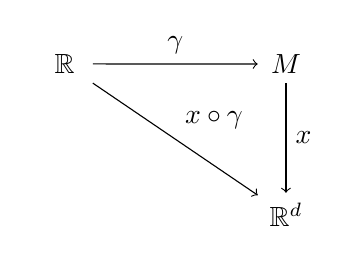
\begin{tikzpicture}
  \matrix (m) [matrix of math nodes, row sep=4em, column sep=6em, minimum width=2em]
  {
 \mathbb{R} & M   \\
&  \mathbb{R}^d \\ 
};
  \path[->]  
  (m-1-1) edge node [auto] {$\gamma$} (m-1-2)
          edge node [auto] {$x\circ \gamma$} (m-2-2)
  (m-1-2) edge node [auto] {$x$} (m-2-2);
\end{tikzpicture}
EY: 20151109 Schuller was explaining that the trajectory is real in $M$; the coordinate maps to obtain coordinates is $x\circ \gamma$

\subsection{4. Diffeomorphisms}

$M \xrightarrow{ \phi } N$

If $M,N$ are naked sets, the structure preserving maps are the bijections (invertible maps).  

e.g. $\lbrace 1,2,3 \rbrace \to \lbrace a,b \rbrace$

\begin{definition}
  $M \cong_{\text{set}} N$ (set-theoretically) isomorphic if $\exists \, $ bijection $\phi : M \to N$
\end{definition}

\underline{Examples}.  $\mathbb{N} \cong_{\text{set}} \mathbb{Z}$ \\
$\mathbb{N} \cong_{\text{set}} \mathbb{Q}$  (EY: 20151109 Schuller says from diagonal counting)\\
$\mathbb{N} \cancel{\cong_{\text{set}}} \mathbb{R}$

Now $(M, \mathcal{O}_M) \cong_{\text{top}} (N,\mathcal{O}_N)$ (topl.) isomorphic $=$ ``homeomorphic'' $\exists \, $ bijection $\phi : M \to N$  \\
\phantom{ \quad \quad \, } $\phi, \phi^{-1}$ are continuous.  

$(V,+,\cdot) \cong_{\text{vec}} ( W,+_w,\cdot_w)$ (EY: 20151109 vector space isomorphism) if \\
$\exists \, \text{ bijection } \phi : V \to W$ linearly

\underline{finally}

\begin{definition}
  Two $C^{\infty}$-manifolds \\
  $(M,\mathcal{O}_M, \mathcal{A}_M)$ and $(N,\mathcal{O}_N, \mathcal{A}_N)$ are said to be \textbf{diffeomorphic} if $\exists \, $ bijection $\phi : M \to N$ s.t. 
\[
\begin{aligned} & \phi : M \to N \\
  & \phi^{-1} : N \to M \end{aligned}
    \]
are both $C^{\infty}$-maps

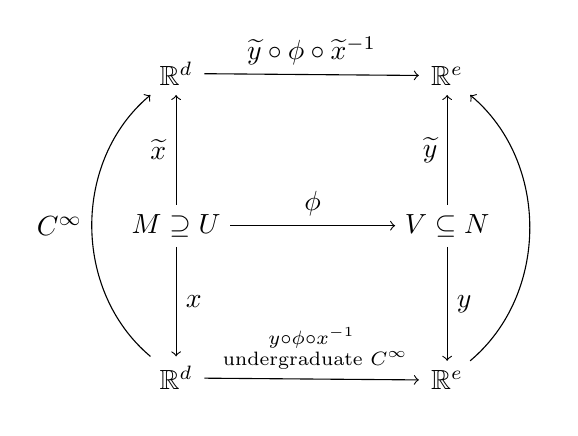
\begin{tikzpicture}
  \matrix (m) [matrix of math nodes, row sep=4em, column sep=6em, minimum width=2em]
  {
 \mathbb{R}^d & \mathbb{R}^e   \\
M \supseteq U &  V\subseteq N   \\ 
\mathbb{R}^d & \mathbb{R}^e \\
};
  \path[->]  
  (m-1-1) edge node [auto] {$\widetilde{y} \circ \phi \circ \widetilde{x}^{-1}$} (m-1-2)
  (m-2-1) edge node [auto] {$\widetilde{x}$} (m-1-1)
          edge node [auto] {$\phi$} (m-2-2)
          edge node [auto] {$x$} (m-3-1)
  (m-3-1) edge node [auto] {$ \substack{ y\circ \phi \circ x^{-1} \\ 
 \text{ undergraduate } C^{\infty} }$} (m-3-2)
          edge [bend left=50] node [auto] {$C^{\infty}$} (m-1-1)
  (m-2-2) edge node [auto] {$\widetilde{y}$} (m-1-2) 
          edge node [auto] {$y$} (m-3-2)
  (m-3-2) edge [bend right=50] node [auto] {$$} (m-1-2);
\end{tikzpicture}


\end{definition}

\begin{theorem}
  $\# = $ number of $C^{\infty}$-manifolds one can make out of a given $C^0$-manifolds (if any) - up to diffeomorphisms.  

\begin{tabular}{l | c r }
  $\text{dim}M$ &  $\#$ &  \\
  \hline
  1  & 1  & Morse-Radon theorems \\
 2  & 1  & Morse-Radon theorems \\
 3 & 1  & Morse-Radon theorems \\
4 & uncountably infinitely many & \\
5 &   finite  & surgery theory \\
6 &  finite & surgery theory \\
\vdots & finite & surgery theory
\end{tabular}

\end{theorem}

EY : 20151109 cf. \url{http://math.stackexchange.com/questions/833766/closed-4-manifolds-with-uncountably-many-differentiable-structures}  \\
\href{http://www.maths.ed.ac.uk/~aar/papers/scorpan.pdf}{The wild world of 4-manifolds}


\section*{Tutorial 4 Differentiable Manifolds}

EY : 20151109 The \url{gravity-and-light.org} website, where you can download the tutorial sheets \emph{and} the full length videos for the tutorials and lectures, are no longer there.  $=($  

Hopefully, the YouTube video will remain: \url{https://youtu.be/FXPdKxOq1KA?list=PLFeEvEPtX_0RQ1ys-7VIsKlBWz7RX-FaL}

\exercisehead{1: True or false?} \emph{These basic questions are designed to spark discussion and as a self-test.}

Tick the correct statements, but not the incorrect ones!

\begin{enumerate}
  \item[(a)] The function $f: \mathbb{R} \to \mathbb{R}$, \dots
    \begin{itemize}
      \item  
      \item
      \item \dots , defined by $f(x) = |x^3|$, lies in $C^3(\mathbb{R} \to \mathbb{R})$.  

EY : 20151109 \solutionhead{1a3} For $f: \mathbb{R} \to \mathbb{R}$, $f(x) = |x^3| = \begin{cases} x^3 & \text{ if } x \geq 0 \\
  -x^3 & \text{ if } x < 0 \end{cases}$ 
\[
\begin{aligned}
  & f'(x) = \begin{cases} 3x^2  & \text{ if } x \geq 0 \\
    -3x^2 & \text{ if } x < 0 \end{cases} \\ 
  & f''(x) = \begin{cases} 6x  & \text{ if } x \geq 0 \\
    -6x & \text{ if } x < 0 \end{cases} 
\end{aligned}
\]
Thus, 
\[
\boxed{ f(x) = |x^3| \in C^1(\mathbb{R}) \text{ but } f(x) \notin C^2(\mathbb{R}) \subseteq C^3(\mathbb{R}) }
\]
      \item
      \item
\end{itemize}
  \item[(b)]
  \item[(c)]
\end{enumerate}

\textbf{Short} \exercisehead{4: Undergraduate multi-dimensional analysis }

\emph{A good notation and basic results for partial differentiation}.

For a map $f: \mathbb{R}^d \to \mathbb{R}$ we denote by the map $\partial_i f: \mathbb{R}^d \to \mathbb{R}$ the partial derivative with respect to the $i$-th entry.

\questionhead{:} Given a function
\[
f: \mathbb{R}^3 \to \mathbb{R}; \, (\alpha, \beta, \delta) \mapsto f(\alpha,\beta,\delta) := \alpha^3\beta^2 + \beta^2 \delta + \delta
\]
calculate the values of the following derivatives:

\solutionhead{:}

\begin{itemize}
  \item $(\partial_2f)(x,y,z) = $
  \item $(\partial_1f)(\square,\circ,*) =$
  \item $(\partial_1 \partial_2 f)(a,b,c) = $ 
  \item $(\partial_3^2 f)(299,1222,0) =$
\end{itemize}

EY: 20151110

For $f(\alpha,\beta,\delta) := \alpha^3\beta^2 + \beta^2 \delta + \delta$, or $f(x,y,z) = x^3 y^2 + y^2 z + z$, 
\[
\begin{aligned}
  & (\partial_2 f) = 2(x^3y+yz) \\ 
  & (\partial_1 f) = 3x^2 y^2 \\ 
  & (\partial_1\partial_2 f) = 6x^2 y \\ 
  & (\partial_3^2f) = 0 
\end{aligned}
\]
and so 
\begin{itemize}
  \item $(\partial_2f)(x,y,z) = 2(x^3 y + yz)  $
  \item $(\partial_1f)(\square,\circ,*) = 3\square^2 \circ^2$
  \item $(\partial_1 \partial_2 f)(a,b,c) = 6a^2 b$ 
  \item $(\partial_3^2 f)(299,1222,0) = 0$
\end{itemize}



\exercisehead{5: Differentiability on a manifold}

\emph{How to deal with functions and curves in a chart} 

Let $(M, \mathcal{O}, \mathcal{A})$ be a smooth $d$-dimensional manifold.  Consider a chart $(U,x)$ of the atlas $\mathcal{A}$ together with a smooth curve $\gamma : \mathbb{R} \to U$ and a smooth function $f:U \to \mathbb{R}$ on the domain $U$ of the chart. 

\questionhead{:} Draw a commutative diagram containing the chart domain, chart map, function, curveand the respective representatives of the function and the curve in the chart. 

\solutionhead{:}

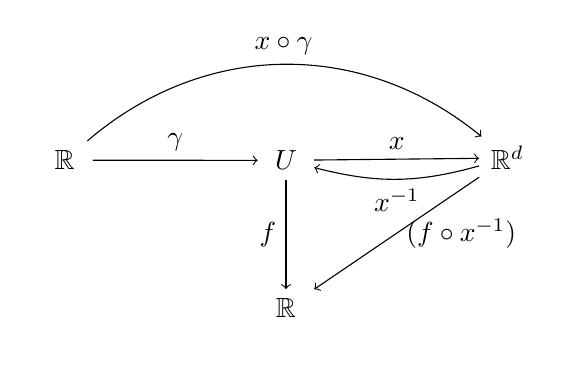
\begin{tikzpicture}[decoration=snake]
  \matrix (m) [matrix of math nodes, row sep=4em, column sep=6em, minimum width=2em]
  {
 \mathbb{R} & U & \mathbb{R}^d \\
& \mathbb{R} &  \\
};
  \path[->]
  (m-1-1) edge node [above] {$\gamma$} (m-1-2)
          edge [bend left=40] node [auto] {$x\circ \gamma$} (m-1-3)
  (m-1-3) edge [bend left=15] node [auto] {$x^{-1}$} (m-1-2)
          edge node [right] {$(f\circ x^{-1})$ } (m-2-2)
  (m-1-2) edge node [left] {$f$} (m-2-2)
          edge node [auto] {$x$} (m-1-3);
\end{tikzpicture} \quad \quad \, 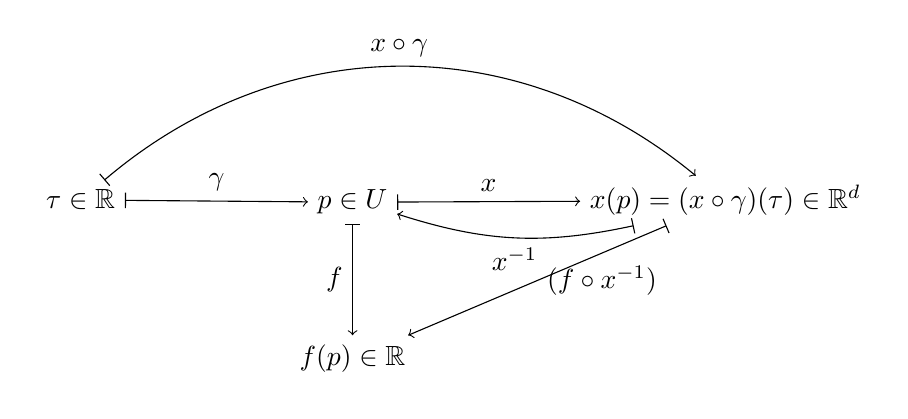
\begin{tikzpicture}[decoration=snake]
  \matrix (m) [matrix of math nodes, row sep=4em, column sep=6em, minimum width=2em]
  {
 \tau \in \mathbb{R} & p \in U & x(p) = (x\circ \gamma)(\tau) \in \mathbb{R}^d \\
& f(p) \in \mathbb{R} &  \\
};
  \path[|->]
  (m-1-1) edge node [above] {$\gamma$} (m-1-2)
          edge [bend left=40] node [auto] {$x\circ \gamma$} (m-1-3)
  (m-1-3) edge [bend left=15] node [auto] {$x^{-1}$} (m-1-2)
          edge node [right] {$(f\circ x^{-1})$ } (m-2-2)
  (m-1-2) edge node [left] {$f$} (m-2-2)
          edge node [auto] {$x$} (m-1-3);
\end{tikzpicture}



\questionhead{:} Consider, for $d=2$,
\[
(x\circ \gamma)(\lambda):= (\cos{(\lambda)}, \sin{(\lambda)} ) \text{ and } (f\circ x^{-1})((x,y)) := x^2 +y^2
\]
Using the chain rule, calculate
\[
(f\circ \gamma)'(\lambda)
\]
explicitly.

\solutionhead{:}

EY : 20151109 Indeed, the domains and codomains of this $f\gamma$ mapping makes sense, from $\mathbb{R} \to \mathbb{R}$ for 
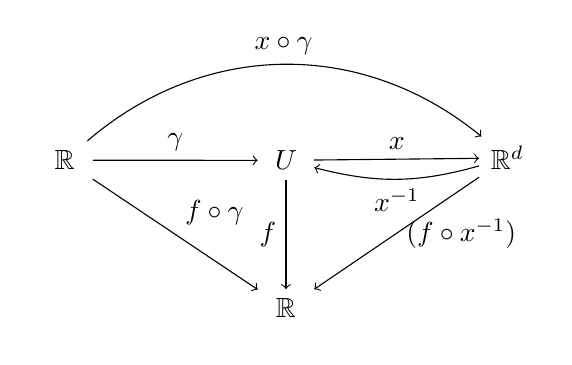
\begin{tikzpicture}[decoration=snake]
  \matrix (m) [matrix of math nodes, row sep=4em, column sep=6em, minimum width=2em]
  {
 \mathbb{R} & U & \mathbb{R}^d \\
& \mathbb{R} &  \\
};
  \path[->]
  (m-1-1) edge node [above] {$\gamma$} (m-1-2)
          edge [bend left=40] node [auto] {$x\circ \gamma$} (m-1-3)
          edge node [auto] {$f\circ \gamma$} (m-2-2)
  (m-1-3) edge [bend left=15] node [auto] {$x^{-1}$} (m-1-2)
          edge node [right] {$(f\circ x^{-1})$ } (m-2-2)
  (m-1-2) edge node [left] {$f$} (m-2-2)
          edge node [auto] {$x$} (m-1-3);
\end{tikzpicture} \quad \quad \, 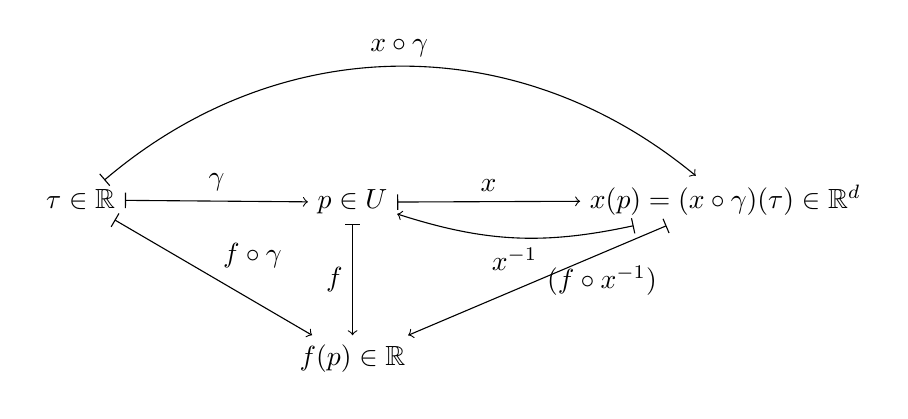
\begin{tikzpicture}[decoration=snake]
  \matrix (m) [matrix of math nodes, row sep=4em, column sep=6em, minimum width=2em]
  {
 \tau \in \mathbb{R} & p \in U & x(p) = (x\circ \gamma)(\tau) \in \mathbb{R}^d \\
& f(p) \in \mathbb{R} &  \\
};
  \path[|->]
  (m-1-1) edge node [above] {$\gamma$} (m-1-2)
          edge [bend left=40] node [auto] {$x\circ \gamma$} (m-1-3)
          edge node [auto] {$f\circ \gamma$} (m-2-2)
  (m-1-3) edge [bend left=15] node [auto] {$x^{-1}$} (m-1-2)
          edge node [right] {$(f\circ x^{-1})$ } (m-2-2)
  (m-1-2) edge node [left] {$f$} (m-2-2)
          edge node [auto] {$x$} (m-1-3);
\end{tikzpicture}

\[
\begin{gathered}
  (f\circ \gamma)'(\lambda) = (Df)\cdot \dot{\gamma}(\lambda) = \frac{ \partial f}{ \partial x^j} \dot{\gamma}^j(\lambda) = 2x (-\sin{\lambda} ) + 2y \cos{\lambda} = 2(-\cos{\lambda} \sin{\lambda} + \sin{\lambda} \cos{\lambda} ) = 0 
\end{gathered}
\]



\section{Lecture 5: Tangent Spaces}

lead question: ``what is the velocity of a curve $\gamma$ \@ point $p$?

\subsection{Velocities}

\begin{definition}
  $(M,\mathcal{O},\mathcal{A})$ smooth mfd. \\
  curve $\gamma : \mathbb{R} \to M$ at least $C^1$.   \\
  Suppose $\gamma(\lambda_0) =p$ \\
  The \textbf{velocity} of $\gamma$ \@ $p$ is the linear map 
\[
\begin{gathered}
v_{\gamma, p} : C^{\infty}(M) \xrightarrow{ \sim } \mathbb{R}
\end{gathered}
\]
$C^{\infty}(M) := \lbrace f: M \to \mathbb{R} | f \text{ smooth function } \rbrace$ equipped with $\begin{gathered}  \quad \\ 
   (f\oplus g)(p) := f(p) + g(p) \\
   (\lambda \otimes g)(p) := \lambda \cdot g(p) \end{gathered}$

$\sim$ denotes linear map on top of $\xrightarrow{}$.

\[
f \mapsto v_{\gamma,p}(f):= (f\circ \gamma)'(\lambda_0)
\]


\end{definition}

intuition
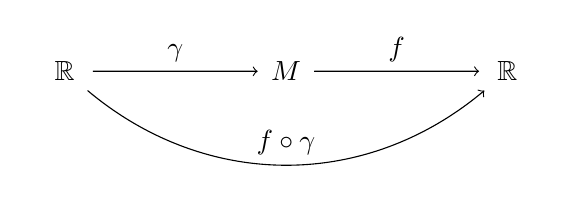
\begin{tikzpicture}
  \matrix (m) [matrix of math nodes, row sep=4em, column sep=6em, minimum width=2em]
  {
 \mathbb{R} & M  & \mathbb{R}   \\
};
  \path[->]  
  (m-1-1) edge node [auto] {$\gamma$} (m-1-2)
          edge [bend right=40] node [auto] {$f\circ \gamma $} (m-1-3)
  (m-1-2) edge node [auto] {$f $} (m-1-3);
\end{tikzpicture}



Schuller says: children run around the world.  Temperature function as temperature contour lines.  You feel the temperature.  You observe the rate of change of temperature as you run around.  $f$ is temperature.  

\underline{past}: `` $\underbrace{v^i}_{} (\partial_i f) = (\underbrace{v^i \partial_i}_{\text{vector}})f$ 

\subsection{Tangent vector space}

\begin{definition}
  For each point $p \in M$ \\
def the \textbf{set} ``tangent space $\neq_0 M$ \@ $p$ ``
\[
T_p M := \lbrace v_{\gamma, p} | \gamma \text{ smooth curves } \rbrace
\]
\end{definition}

\underline{picture}:\\
rather $M$ than (embedded) $p$ $T_pM$ EY : 20151109 see \url{https://youtu.be/pepU_7NJSGM?t=12m38s} for the picture

\underline{Observation}: $T_pM$ can be made into a vector space. 

\[
\begin{aligned}
& \begin{aligned}
  \oplus : & T_pM \times T_pM \to   \\
  & (v_{\gamma,p} \oplus v_{\delta,p})(\underbrace{f}_{ \in C^{\infty}(M)} ) := v_{\gamma,p}(f) +_{\mathbb{R}} v_{\delta,p}(f) \\
  \end{aligned} \\
& \begin{aligned}
    \odot : & \mathbb{R} \times T_pM \to \text{Hom}(C^{\infty}(\mathbb{R}),\mathbb{R}) \\
    & (\alpha \odot v_{\gamma,p} )(f) := \alpha \cdot_{\mathbb{R}}  v_{\gamma, p}(f)
\end{aligned}
\end{aligned}
\]
Remains to be shown that 
\begin{enumerate}
  \item[(i)] $\exists \, \sigma$ curve : $v_{\gamma,p} \oplus v_{\delta,p} = v_{\sigma,p}$
  \item[(ii)] $\exists \, \tau $ curve : $\alpha \odot v_{\gamma,p} = v_{\tau,p}$
\end{enumerate}

\underline{Claim}: $\begin{aligned} & \quad \\ 
  \tau : \mathbb{R}&  \to M  \\
  & \mapsto \tau(\lambda) := \gamma(\alpha  \lambda + \lambda_0) = (\gamma \circ \mu_{\alpha})(\lambda)
\end{aligned}$
where $\begin{aligned} & \quad \\
   \mu_{\alpha}: & \mathbb{R} \to \mathbb{R} \\ 
   & r \mapsto \alpha \cdot r + \lambda_0 \end{aligned}$, 
does the trick.

$\tau(0) = \gamma(\lambda_0) =p$

\[
\begin{aligned}
  v_{\tau,p} & := (f\circ \tau)'(0) = (f\circ \gamma \circ \mu_{\alpha} )'(0) \\ 
  & =  (f\circ \gamma)'(\lambda_0) \cdot \alpha = \\
  & = \alpha \cdot v_{\gamma,p}
\end{aligned}
\]

Now for the sum: %(EY:20151109 ??)

$v_{\gamma,p} \oplus v_{\delta,p} \overset{?}{=} v_{\sigma, p} $

make a \underline{choice} of chart $(\underbrace{U}_{\ni p} , x)$  In cloud: ill definition alarm bells. 

and define:

Claim:
\[
\begin{aligned}
  & \sigma : \mathbb{R} \to M \\
  & \sigma(\lambda) := x^{-1}( \underbrace{ (x\circ \gamma)(\lambda_0 + \lambda)}_{\mathbb{R} \to \mathbb{R}^d}  + (x\circ \delta)(\lambda_1+ \lambda) - (x\circ \gamma)(\lambda_0) )
\end{aligned}
\]
does the trick.
\begin{proof}
Since: 
\[
\begin{aligned}
  \sigma_x(0) & = x^{-1}((x\circ \gamma)(\lambda_0) + (x\circ \delta)(\lambda_1) - (x\circ \gamma)(\lambda_0)) \\
  & = \delta(\lambda_1) = p \end{aligned}
\]
Now:
\[
\begin{aligned}
  v_{\sigma_x,p}(f) & := (f\circ \sigma_x)'(0) =  \\ 
  & = ( \underbrace{ (f\circ x^{-1}) }_{\mathbb{R}^d \to \mathbb{R}}  \circ \underbrace{ (x\circ \sigma_x) }_{\mathbb{R} \to \mathbb{R}^d}  )'(\gamma) = \underbrace{ (x\circ \sigma_x)'(0) }_{(x\circ \gamma)'(\lambda_0) + (x\circ \delta)'(\lambda_1) } \cdot \left( \partial_i (f\circ x^{-1}) \right)(x( \underbrace{ \sigma(0)}_{p} ) ) = \\
  & = (x\circ \gamma)'(\lambda_0)(\partial_i (f\circ x^{-1}) )(x(p)) + (x\circ \delta)(\lambda_1)(\partial_i (f\circ x^{-1})  )(x(p)) \\
  & = (f\circ \gamma)'(\lambda_0) + (f\circ \delta)'(\lambda_1) = \\
  & = v_{\gamma,p}(f) + v_{\delta,p}(f) \quad \, \forall \, f \in C^{\infty}(M)
\end{aligned}
\]

\[
\boxed{ v_{\gamma,p} \oplus v_{\delta,p} = v_{\sigma, p} }
\]
\end{proof}

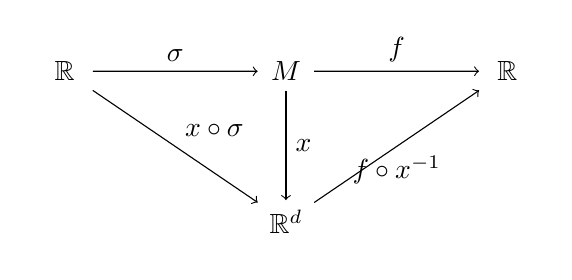
\begin{tikzpicture}
  \matrix (m) [matrix of math nodes, row sep=4em, column sep=6em, minimum width=2em]
  {
     \mathbb{R} & M  & \mathbb{R}   \\
     & \mathbb{R}^d & \\ 
};
  \path[->]  
  (m-1-1) edge node [auto] {$\sigma$} (m-1-2)
          edge  node [auto] {$x\circ \sigma $} (m-2-2)
  (m-1-2) edge node [auto] {$x $} (m-2-2)
          edge node [auto] {$f$} (m-1-3)
  (m-2-2) edge node [below] {$f\circ x^{-1}$} (m-1-3);
\end{tikzpicture}


\underline{picture}: (cf. \url{https://youtu.be/pepU_7NJSGM?t=39m5s})

\[
\begin{aligned} 
  \gamma : \mathbb{R} \to M \\
  \delta : \mathbb{R} \to M \end{aligned}
\]
$(\gamma \oplus)(\lambda) := \gamma(\lambda) + \delta(\lambda)$

EY : 20151109 Schuller says adding trajectories is chart dependent, bad. Adding velocities is good.  
\subsection{Components of a vector wrt a chart}

\begin{definition}
  Let $(U,x) \in \mathcal{A}_{\text{smooth}}$.  \\
  Let $\begin{aligned} & \gamma : \mathbb{R} \to U \\ 
    & \gamma(0) = p \end{aligned}$.  

Calculate 
\[
\begin{aligned} 
  v_{\gamma,p}(f) & := (f \circ \gamma)'(0) = (\underbrace{ (f\circ x^{-1}) }_{\mathbb{R}^d \to \mathbb{R} }  \circ \underbrace{ (x\circ \gamma)}_{\mathbb{R} \to \mathbb{R}^d}  )'(0) \\
  & = \underbrace{ (x\circ \gamma)^{i'}(0) }_{\dot{\gamma}_x^i(0) }  \cdot \underbrace{ (\partial_i(f\circ x^{-1} ) )(x(p))  }_{ =: \left( \frac{ \partial f}{ \partial x^i } \right)_p }
\end{aligned}
\]
think cloud $f:M\to \mathbb{R}$
\[
 = \boxed{ \dot{\gamma}_x^i(0) \cdot \left( \frac{ \partial }{ \partial x^i} \right)_p } f \quad \, \forall \, f \in C^{\infty}(M)
\]
$\therefore$ as a map.  

\[
v_{\gamma,p} \underbrace{=}_{\text{use of chart} } \underbrace{ \gamma_x^i(0) }_{ \text{ ``components of the velocity $v_{\gamma,p}$'' } } \underbrace{ \left( \frac{ \partial }{ \partial x^i} \right)}_{ \substack{ \text{ basis elements of the $T_pM$ wrt which the components need to be understood.} \\
\text{ ``chart induced basis of $T_pM$''} } } 
\]
\end{definition}

Picture: \url{https://youtu.be/pepU_7NJSGM?t=1h16s}

\subsection{4. Chart-induced basis}

\begin{definition}
  $(U,x) \in \mathcal{A}_{\text{smooth}}$ \\
the $\left( \frac{ \partial }{ \partial x^1} \right)_p , \dots , \left( \frac{ \partial }{ \partial x^d} \right)_p \in T_pU \subseteq T_pM$

constitute a \textbf{basis} of $T_pU$

\end{definition}

\begin{proof} remains: linearly independent 
  \[
\begin{gathered}
\lambda^i \left( \frac{ \partial }{ \partial x^i} \right)_p \overset{!}{=} 0  \\
 \Longrightarrow \lambda^i \left( \frac{ \partial }{ \partial x^i} \right)_p(x^j) = \lambda^i \partial_i (\underbrace{ x^j \circ x^{-1} }_{} )( x(p)) = \\
 = \lambda^i \delta_i^{\,\,j} = \lambda^j \quad \quad \, j = 1 , \dots , d
\end{gathered} \quad \quad \, \begin{gathered}
  x^j \circ x^{-1} : \mathbb{R}^d \to \mathbb{R} \\
  (\alpha^1 , \dots , \alpha^d) \mapsto \alpha^j 
\end{gathered}
\]
in cloud: $x^j : U \to \mathbb{R}$ differentiable




\end{proof}


\begin{corollary}
 $ \text{dim}T_pM = d = \text{dim}M$
\end{corollary}

\underline{Terminology}: $X \in T_pM$ $\to $ $\exists \, \gamma : \mathbb{R} \to M : X = v_{\gamma,p}$ and \\
\phantom{\underline{Terminology}:} $\exists \, \underbrace{ X_1^1 , \dots , X^d }_{\in \mathbb{R} } : X = X^i \left( \frac{ \partial }{ \partial x^i} \right)_p$



\subsection{5. Change of vector \emph{\underline{components}} under a change of chart}

\ding{56} vector does \textbf{not} change under change of chart.

Let $(U,x)$ and $(V,y)$ be overlapping charts and $p \in U\cap V$.  \\
Let $X \in T_pM$

\[
X^i_{(y)}\cdot \left( \frac{ \partial }{ \partial y^i} \right)_p \underbrace{=}_{(V,y)} X \underbrace{=}_{ (U,x) } X^i_{x} \left( \frac{ \partial }{ \partial x^i} \right)_p
\]
to study change of components formula:
\[
\begin{aligned}
  \left( \frac{ \partial }{ \partial x^i} \right)_p f & = \partial_i(f\circ x^{-1} )(x(p)) =  \\
  & = \partial_i (\underbrace{ (f\circ y^{-1}) }_{\mathbb{R}^d \to \mathbb{R} } \circ (\underbrace{ y\circ x^{-1}}_{\mathbb{R}^d \to \mathbb{R}^d} )(x(p)) \\
  & = (\partial_i (y^i\circ x^{-1} ) )(x(p)) \cdot (\partial_j (f\circ y^{-1}) )(y(p)) = \\
  & = \boxed{ \left( \frac{ \partial y^p}{ \partial x^i} \right)_p \cdot \left( \frac{ \partial f}{ \partial y^j} \right)_p  } f
\end{aligned}
\]
\[
\begin{gathered}
  \Longrightarrow X^i_{(x)} \left( \frac{ \partial y^j}{ \partial x^i} \right)_p \left( \frac{ \partial }{ \partial y^j} \right)_p = X^j_{(y)}\left( \frac{ \partial }{ \partial y^j} \right)_p \\
  \Longrightarrow \boxed{ X^j_{(y)} = \left( \frac{ \partial y^j}{ \partial x^i} \right)_pX^i_{(x)} }
\end{gathered}
\]

\subsection{6. Cotangent spaces }

$T_pM = V$

trivial $(T_pM)^* := \lbrace \varphi : T_pM \xrightarrow{\sim} \mathbb{R} \rbrace$

\underline{Example}: $f\in C^{\infty}(M)$ 

\[
\begin{aligned}
  (df)_p : & T_p M \xrightarrow{ \sim } \mathbb{R} \\ 
  & X \mapsto (df)_p(X)
\end{aligned}
\]
i.e. $\boxed{ (df)_p \in T_pM^* } $

$(df)_p$ called the gradient of $f$ \@ $p\in M$.  

Calculate components of gradient w.r.t. chart-induced basis $(U,x)$  

\[
\begin{aligned}
  \left( (df)_p \right)_j & := (df)_p\left( \left( \frac{ \partial }{ \partial x^j} \right)_p \right) \\
  & = \left( \frac{ \partial f}{ \partial x^j } \right)_p = \partial_j (f\circ x^{-1} )(x(p))
\end{aligned}
\]

\begin{theorem}
  Consider chart $(U,x)  \Longrightarrow x^i : U \to \mathbb{R}$  

\underline{Claim}: $(d x^1)_p, (dx^2)_p, \dots , (dx^d)_p$ basis of $T_p^*M$ 

$\Longrightarrow $ In fact: dual basis: 
\[
(dx^a)_p \left( \left( \frac{ \partial }{ \partial x^b} \right)_p \right) = \left( \frac{ \partial x^a}{ \partial x^b} \right)_p = \dots = \delta_b^a
\]
\end{theorem}

\subsection{ 7. Change of \emph{ \underline{components} } of a covector under a change of chart: }

\[
\begin{gathered}
  \underbrace{ T_p^*M }_{ \ni \omega} \text{ with } 
\omega_{(y)} (dy^j)_p =   \omega = \omega_{(x)i} (dx^i)_p  \\
\Longrightarrow \boxed{ \omega_{(y)i} = \frac{ \partial x^j}{ \partial y^i } \omega_{(x)j } }
\end{gathered}
\]

 






\section{Lecture 6: Fields}

So far: 

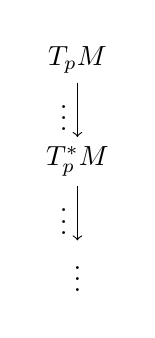
\begin{tikzpicture}[decoration=snake]
  \matrix (m) [matrix of math nodes, row sep=2em, column sep=3em, minimum width=1em]
  {
T_pM \\ 
T_p^*M \\
\vdots \\
};
  \path[->] %,decorate={zigzag,amplitude=0.7pt, segment length=1.2mm, pre=lineto,pre length=4pt}]
  (m-1-1) edge node [left] {$\vdots$} (m-2-1)
  (m-2-1) edge node [left] {$\vdots$} (m-3-1);
\end{tikzpicture},

now

in Thought Cloud: theory of bundles

\subsection{Bundles}

\begin{definition}
  A \textbf{bundle} is a triple 
\[
E \xrightarrow{ \pi } M 
\]
$E$ smooth manifold \quad \, ``\textbf{total space}'' \\
$\pi$ smooth map (surjective)  ``projection map'' \\
$M$ smooth manifold ``base space''

\end{definition}

\underline{Example} $E = $ cylinder
$M = $ circle


\begin{definition}
  define \textbf{fibre over $p$} \\
  \phantom{define} $:= \text{preim}_{\pi}(\lbrace p \rbrace)$
\end{definition}

\begin{definition}
A \textbf{section} $\sigma$ of a bundle

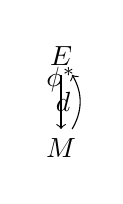
\begin{tikzpicture}
  \matrix (m) [matrix of math nodes, row sep=2em, column sep=3em, minimum width=1em]
  {
    E \\
    M \\ };
  \path[->]
  (m-1-1) edge node [above] {$\phi^*$} (m-2-1)
  (m-2-1) edge [bend right=30] node [left] {$d$} (m-1-1);
\end{tikzpicture}





require $\pi \circ \sigma = \text{id}_M$
\end{definition}

Schuller says: in quantum mechanics, 
\underline{Aside}: $\psi : M \to \mathbb{C}$


\subsection{Tangent bundle of smooth manifold}

$(M,\mathcal{O},\mathcal{A})$ smooth manifold

\begin{enumerate}
\item[(a)] as a \textbf{set}
  $TM : = \dot{\bigcup}_{p\in M} T_pM$
\item[(b)] $\begin{aligned} & \quad \\
  \text{surjective } & \pi: TM \to M \\
  & X\mapsto p \end{aligned}$ the \emph{unique} point $p\in M$, $X \in T_pM$  

\underline{situation}:  $\underbrace{TM}_{\text{set}} \underbrace{ \xrightarrow{ \pi } }_{\text{surjective map }} \underbrace{M}_{\text{smooth manifold}}$

\item[(c)] Construct topology on $TM$ that is the coarsest topology such that $\pi$ (just) continuous.  (``initial topology with respect to $\pi$'').

\[
\mathcal{O}_{TM} := \lbrace \text{preim}_{\pi}(U) | \mathcal{U}\in \mathcal{O} \rbrace
\]
Show: Tutorial $\mathcal{O}_{TM}$
Schuller says this is shown in the tutorial

$(TM,\mathcal{O}_{TM})$  \\

\underline{Construction of a $C^{\infty}$-atlas on $TM$ from the $C^{\infty}$-atlas $\mathcal{A}$ on $M$. }

\[
\mathcal{A}_{TM} := \lbrace (T\mathcal{U},\xi_x  ) | (U,x) \in \mathcal{A} \rbrace
\]
where
\[
\begin{aligned}
  \xi_x : & T \mathcal{U} \to \mathbb{R}^{2\cdot\text{dim}  M } \\
  & X \mapsto (\underbrace{ (x^1 \circ \pi)(X), \dots, (x^d\circ \pi)(X) }_{(U,x)-\text{ coords of $\pi(X)$ } \, (d \text{ many } ) } , (dx^1)_{\pi(X)}(X), \dots , (dx^d)_{\pi(X)}(X)  )
\end{aligned}
\]
where $X\in T_{\pi(X)}M$ \\
\phantom{where } $X = X_{(x)}^i \left( \frac{ \partial }{ \partial x^i} \right)_{\pi(X)}$  \\
\phantom{where } $\begin{aligned} \quad  & \\
  (dx^j)_{\pi(X)}(X) &= (dx^j)_{\pi(X)} \left( X^i_{(x)}\left( \frac{ \partial }{ \partial x^i} \right)_{\pi(X)} \right) = \\
  & = X^i_{(x)}\delta_i^j = X^j_{(x)}\end{aligned}$

\underline{Write} $\xi_x^{-1} : \xi_x(TU) \subseteq \mathbb{R}^{2\text{dim}M} \to TU$
\[
(\alpha^1 , \dots , \alpha^d, \beta^1, \dots , \beta^d) := \beta^i \left( \frac{ \partial }{ \partial x^i} \right)_{ \underbrace{ x^{-1}(\alpha^1 , \dots , \alpha^d) }_{\pi(X)} }
\]

\underline{Check}: \[
\begin{gathered}
  (\xi_y \circ \xi_x^{-1})(\alpha^1 , \dots , \alpha^d, \beta^1, \dots , \beta^d) = \\
  = \xi_y \left( \beta^i \left( \frac{ \partial }{ \partial x^i} \right)_{x^{-1}(\alpha^1 , \dots , \alpha^d) } \right) \\
  = \left( \dots, (y^i \circ \pi)( \beta^m \cdot \left( \frac{ \partial }{ \partial x^m} \right)_{x^{-1}(\alpha^1 \dots \alpha^d) } )  , \dots , \dots (dy^i)_{x^{-1}(\alpha^1, \dots \alpha^d) } \left( \beta^m \left( \frac{ \partial }{ \partial x^m} \right)_{x^{-1}(\alpha^1 \dots \alpha^d) } \right) , \dots   \right) = \\
  = ( \dots , (y^i \circ x^{-1})(\alpha^1 , \dots , \alpha^d), \dots , \dots , \underbrace{ \beta^m(dy^i)_{x^{-1} (\alpha^1, \dots , \alpha^d) } \left( \left( \frac{ \partial }{ \partial x^m} \right)_{x^{-1}(\alpha^1 \dots \alpha^d) } \right)}_{ \beta^m \left( \frac{ \partial y }{ \partial x^m } \right)_{x^{-1}(\alpha^1 \dots \alpha^d)} }  ) 
\end{gathered}
\]

%
$\left( \frac{ \partial y }{ \partial x^m } \right)_{x^{-1}(\alpha^1 \dots \alpha^d)} = \partial_m (y^i \circ x^{-1} )( x\circ (x^{-1}(\alpha^1 \dots \alpha^d) ) ) = \partial_m (y^i \circ x^{-1} )( \alpha^1 \dots \alpha^d)$ smooth.  

\underline{upshot}

\[
\underbrace{TM}_{\text{smooth manifold}} \underbrace{ \xrightarrow{\pi} }_{\text{smooth map} } \underbrace{M}_{\text{ smooth manifold} }
\]
bundle, called the tangent bundle.

\end{enumerate}

\subsection{Vector fields}

\begin{definition}
  A \textbf{smooth vector field} $\chi$ is a \emph{smooth} map
\end{definition}

\subsection{The $C^{\infty}(M)$-module $\Gamma(TM)$}

\textbf{set} $\Gamma(TM) = \lbrace \chi \quad \, M \to TM | \text{ smooth section } \rbrace$
 
$(\chi \oplus \widetilde{\chi})(f) := (\chi f) + \underbrace{\widetilde{\chi}}_{C^{\infty}(M)}(f)$ \\

$(g\odot \xi)(f) := g \cdot \underbrace{ \chi }_{C^{\infty}(M)}(f)$


\underline{upshot}: set of all smooth vector fields can be made into a $C^{\infty}(M)$-module.  

\underline{Fact}: \begin{enumerate}
\item[(1)] ZF\underline{C} $\Longrightarrow $ every vector space has a basis. 
\item[(2)] no such result exists for modules.  
\end{enumerate}

This is a shame, because otherwise, we could have chosen (for any manifolds) vector fields, 
\[
\Xi_{(1)}, \dots , \Xi_{(d)} \in \Gamma(TM)
\]
and would be able to write every vector field $\Xi$
\[
\Xi = \underbrace{ f^i }_{\text{ component functions } } \cdot \Xi_{(i)}
\]

\underline{Simple counterexample}

Schuller says: Take a sphere, Morse Theorem, every smooth vector field must vanish at 2 pts. ``mustn't choose a global basis''


\underline{However}: $\begin{aligned} & \quad \\
  & \frac{ \partial }{ \partial x^i} : U \xrightarrow{ \text{ smooth }} TU \\
  & p \mapsto \left( \frac{ \partial }{ \partial x^i } \right)_p
\end{aligned}$

\subsection{Tensor fields}

so far

$\Gamma(M) = $''set of vector fields''  $C^{\infty}(M)$-module

 $\Gamma(T^*M) = $ ``covector fields'' $C^{\infty}(M)$-module

\begin{definition}
An $(r,s)$-tensor field $T$ is a multi-linear map
\[
T:\underbrace{ \Gamma(T^*M) \times \dots \times \Gamma(T^*M) }_{r} \times \Gamma(TM) \times \dots \times \Gamma(TM) \xrightarrow{ \sim } C^{\infty}(M)
\]
\end{definition}

\underline{Example}: $f\in C^{\infty}(M)$ 
\[
\begin{gathered}
  \begin{aligned} 
    df : & \Gamma(TM) \xrightarrow{ \sim } C^{\infty}(M) \\ 
    & \Xi \mapsto df(\Xi) := \Xi [f]
\end{aligned}
\end{gathered}
\]
$df$ ($0,1$)-T.F. (tensor field)

where $(\Xi f)(\underbrace{p}_{ \in M}) := \underbrace{ \Xi(p) }_{ \in T_pM}f$

can check: $df$ is $C^{\infty}-$linear


\section{Lecture 7: Connections}

\[
\begin{aligned}
  & \nabla_X f = Xf = (df)(X) \text{ but (not quite) } \\ 
  & X : C^{\infty}(M) \to C^{\infty}(M) \\ 
  & df : \Gamma(TM) \to C^{\infty}(M) \\
  & \nabla_X : C^{\infty}(M) \to C^{\infty}(M)
\end{aligned}
\]

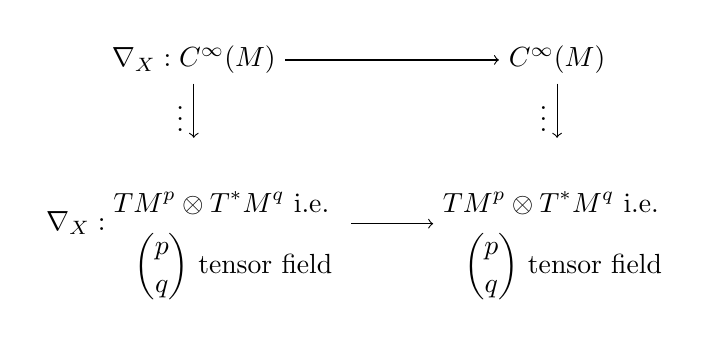
\begin{tikzpicture}[decoration=snake]
  \matrix (m) [matrix of math nodes, row sep=2em, column sep=3em, minimum width=1em]
  {
\nabla_X :   C^{\infty}(M) & C^{\infty}(M)   \\
\nabla_X :  \begin{aligned} \quad  \\ TM^p \otimes T^*M^q \text{ i.e. }  \\  \binom{p}{q} \text{ tensor field }  \end{aligned}   &  \begin{aligned} \quad \\ TM^p \otimes T^*M^q \text{ i.e. }  \\ \binom{p}{q} \text{ tensor field } \end{aligned} \\  };
%  \path[-stealth]
  \path[->]
  (m-1-1) edge node [above] {$$} (m-1-2)
%  edge node [left] {$\text{ev}_0$} (m-2-2)
%  (m-1-1) edge node [left] {$\alpha$} (m-2-1)
  (m-2-1) edge node [below] {$$} (m-2-2);
%  edge node [below] {$\pi_M$} (m-2-2);
  \path[->] %,decorate={zigzag,amplitude=0.7pt, segment length=1.2mm, pre=lineto,pre length=4pt}]
  (m-1-1) edge node [left] {$\vdots$} (m-2-1)
  (m-1-2) edge node [left] {$\vdots$} (m-2-2);
\end{tikzpicture}


\subsection{Directional derivatives of tensor fields}

manifold with connection is quadruple $(M, \mathcal{O}, \mathcal{A}, \nabla)$ 

topology $\mathcal{O}$

atlas $\mathcal{A}$

Consider chart $(U,x) \in \mathcal{A}$

\begin{definition}
$\forall \, $ pair $(X, (p,q)-\text{tensor field}) \equiv (X, (p,q)-TF)$,

\textbf{connection} $\nabla$ on smooth manifold $(M,\mathcal{O},\mathcal{A})$ 

$\nabla: ( X, (p,q)-TF) \to (p,q)-TF$ s.t.

\begin{enumerate}
  \item[(i)] $\nabla_X f = Xf $
  \item[(ii)]  $\nabla_X(T+S) = \nabla_XT + \nabla_XS $ 
\item[(iii)] \[
\nabla_X(T(\omega,Y)) = (\nabla_XT)(\omega,T) + T(\nabla_X\omega, Y) + T(\omega, \nabla_XY)
\]
``Leibnitz'' rule.

As
\[
T\otimes S (\omega_{(1)}\dots \omega_{(p+r)} , Y_{(1)} \dots Y_{(q+s)}) = T(\omega_{(1)} \dots \omega_{(p)}, Y_{(1)} \dots Y_{(q)} ) \cdot S( \omega_{(p+1)} \dots \omega_{(p+r)} , Y_{(q+1)} \dots Y_{(q+s)})
\]
so 
\[
\nabla_X(T\otimes S) = (\nabla_XT)\otimes S + T\otimes \nabla_XS
\]


\item[(iv)] $\nabla_{fX+Z} T = f\nabla_X T + \nabla_Z T$
$C^{\infty}$-linear
\end{enumerate}
\end{definition}

\subsection{New structure on $(M,\mathcal{O},\mathcal{A})$ required to fix $\nabla$}


There are $(\text{dim}M)^3$ many $\Gamma^i_{ \, \, j k}$
\[
\begin{aligned}
&  \Gamma^i_{ \, \, jk} : U \to \mathbb{R} \\ 
&  p \mapsto \left( dx^i ( \nabla_{ \frac{ \partial}{ \partial x} } \frac{ \partial }{ \partial x^j } ) \right)(p)
\end{aligned}
\]

Now $\nabla_{ \frac{ \partial }{ \partial x^m}  }(dx^i) = ?$

\[
\begin{aligned}
  & \underbrace{ \nabla_{  \frac{ \partial }{ \partial x^m} } ( \underbrace{ dx^i \left( \frac{ \partial }{ \partial x^j } \right) }_{ \delta^i_{ \, \, j} } ) }_{ \rotatebox{90}{$\,=$} \quad \, \text{ (iii) } }  = \frac{ \partial }{ \partial x^m} ( \delta^i_{ \, \, j} ) = 0  \\
& = \left( \nabla_{ \frac{ \partial }{ \partial x^m} } dx^i \right)\left( \frac{ \partial }{ \partial x^j} \right) + dx^i (   \underbrace{ \nabla_{ \frac{ \partial }{ \partial x^m } } \frac{ \partial }{ \partial x^j } }_{ \Gamma^q_{ \, jm }\frac{ \partial }{ \partial x^q} }   ) = 0 \\
& \Longrightarrow \left( \nabla_{ \frac{ \partial }{ \partial x^m } } dx^i \right)\left( \frac{ \partial }{ \partial x^j } \right) = - \Gamma^i_{ jm} \\
& \nabla_{ \frac{ \partial }{ \partial x^m} } dx^i = -\Gamma^i_{ jm} dx^j 
\end{aligned}
\]


% \rotatebox{90}{$\,=$}

Hence

\[
\begin{aligned}
  & ( \nabla_X Y)^i = X(Y^i) + \Gamma^i_{j\underbrace{m}_{\text{ last entry goes in direction of $X$ }} } Y^j X^m \\
  & (\nabla_X \omega)_i = X(\omega_i) + - \Gamma^j_{im} \omega_j X^m
\end{aligned}
\]
Note that for the immediately above expression for $(\nabla_X Y)^i$, in the second term on the right hand side, $\Gamma_{jm}^i$ has the last entry at the bottom, $m$ going in the direction of $X$, so that it matches up with $X^m$. This is a good mnemonic to memorize the index positions of $\Gamma$. 

\underline{summary so far}:
\[
\begin{aligned}
  & ( \nabla_X Y)^i = X(Y^i) + \Gamma^i_{jm }  Y^j X^m \\
  & (\nabla_X \omega)_i = X(\omega_i) + - \Gamma^j_{im} \omega_j X^m
\end{aligned}
\]
similarly, by further application of Leibnitz

$T$ a $(1,2)$-TF (tensor field)

\[
\begin{aligned}
  (\nabla_X T)^i_{ \, \, jk } = X(T^i_{ \, \, jk} ) + \Gamma^i_{ \, \, s m } T^s_{ \, \, jk} X^m - \Gamma^s_{ \, \, jm} T^i_{ \, \, sk} X^m - \Gamma^s_{ \, \, km} T^i_{ \,\, js} X^m
\end{aligned}
\]

What is a Euclidean space: \\
$(M = \mathbb{R}^n, \mathcal{O}_{\text{st}}, \mathcal{A})$ smooth manifold. \\
Assume $(\mathbb{R}^n, \text{id}_{\mathbb{R}^n} ) \in \mathcal{A}$ and 
\[
(\Gamma^i_{(x)})_{jk} = dx^i \left( (\nabla_{\text{\underline{E}}})_{ \frac{ \partial }{ \partial x^k} } \frac{ \partial }{ \partial x^j} \right) \overset{!}{=} 0 
\]


\subsection{Change of $\Gamma$'s under change of chart}

$(U,x)$, $(V,y) \in \mathcal{A}$ and $U \cap V \neq \emptyset$

\[
\Gamma^i_{jk}(y) := dy^i \left( \nabla_{ \frac{ \partial}{ \partial y^k} } \frac{ \partial }{ \partial y^j} \right) = \frac{ \partial y^i}{ \partial x^q }dx^q \left( \nabla_{\frac{ \partial x^p}{ \partial y^k}  \frac{ \partial }{ \partial x^p} } \frac{ \partial x^s}{ \partial y^j} \frac{ \partial }{ \partial x^s } \right)
\]

Note $\nabla_{fX}$ is $C^{\infty}$-linear for $fX$

covector $dy^i$ is $C^{\infty}$-linear in its argument
\[
\begin{aligned}
\Longrightarrow \Gamma_{jk}^i(y) & = \frac{ \partial y^i}{ \partial x^q} dx^q \left( \frac{ \partial x^p}{ \partial y^k} \left[ \left( \nabla_{ \frac{ \partial }{ \partial x^p} } \frac{ \partial x^s}{ \partial y^j} \right) \frac{ \partial }{ \partial x^s} + \frac{ \partial x^s}{ \partial y^j} \left( \nabla_{ \frac{ \partial }{ \partial x^p } } \frac{ \partial }{ \partial x^s } \right)  \right] \right) = \\
& = \frac{ \partial y^i}{ \partial x^q} \frac{ \partial x^p }{ \partial y^k} \frac{ \partial }{ \partial x^p } \frac{ \partial x^s}{ \partial y^j } \delta^q_{ \, \, s} + \frac{ \partial y^i}{ \partial x^q} \frac{ \partial x^p }{ \partial y^k} \frac{ \partial x^s}{ \partial y^j} \Gamma^q_{sp}(x)
\end{aligned}
\]


\begin{equation}\label{Eq:WEHCG0703_changeofGamma}
\Gamma^i_{jk}(y) = \frac{ \partial y^i}{ \partial x^q} \frac{ \partial^2 x^q}{ \partial y^j \partial y^k} + \frac{ \partial y^i}{ \partial x^q } \frac{ \partial x^s }{ \partial y^j} \frac{ \partial x^p }{ \partial y^k} \Gamma^q_{sp}(x)
\end{equation}
Eq. (\ref{Eq:WEHCG0703_changeofGamma}) is the change of connection coefficient function under the change of chart $(U\cap V,x) \to (U\cap V,y)$


\subsection{Normal Coordinates}

\subsection*{Tutorial 7 Connections}

\exercisehead{1}\textbf{: True or false?}

\begin{enumerate}
\item[(a)] 
\begin{itemize}
\item $\nabla_{fX}Y = f\nabla_XY$ by definition so $\nabla_{fX} = f\nabla_X$ i.e. $\nabla_X$ is $C^{\infty}(M)$-linear in $X$
\item $f\in C^{\infty}(M)$ is a $(0,0)$-tensor field. $\nabla_Xf = Xf \equiv X(f)$ by definition.
\item If the manifold is flat, I'm assuming that means that the manifold is globally a Euclidean space, and by definition, $\Gamma=0$.
\[
\nabla_X Y = X^j \frac{ \partial }{ \partial x^j} (Y^i) \frac{ \partial }{ \partial x^i } + \Gamma^i_{jk} Y^k X^k \frac{ \partial }{ \partial x^i} = X^j \frac{ \partial Y^i}{ \partial x^j} \frac{ \partial }{ \partial x^i} + 0
\]
and similarly for any $(p,q)$-tensor field, i.e.
\[
\nabla_X T = X^j \frac{ \partial T^{i_1 \dots i_p}_{ j_1 \dots j_q} }{ \partial x^j}
\]
\item \[
\nabla_X f = X^j \frac{ \partial f}{ \partial x^j} = X\cdot \text{grad}(f)
\]
\item $\forall \, (U,x) \in \mathcal{A}$, locally (after working out the first few cases, and doing induction, one can look up the expression for the local form; I found it in Nakahara's \textbf{Geometry, Topology and Physics}, Eq. 7.26, and it needs to be modified for the convention of order of bottom indices for $\Gamma$:
\[
\nabla_{\nu} t^{\lambda_1 \dots \lambda_p }_{ \mu_1 \dots \mu_q} = \partial_{\nu} t^{\lambda_1 \dots \lambda_p}_{ \mu_1 \dots \mu_q} + \Gamma^{\lambda_1}_{ \,  \kappa \nu } t^{\kappa \lambda_2 \dots \lambda_p }_{\mu_1 \dots \mu_q} + \dots + \Gamma^{\lambda_p}_{ \kappa \nu } t^{\lambda_1 \dots \lambda_{p-1} \kappa }_{ \mu_1 \dots \mu_q} - \Gamma^{\kappa}_{  \mu_1 \nu} t^{\lambda_1 \dots \lambda_p }_{ \kappa \mu_2 \dots \mu_q} - \dots - \Gamma^{\kappa}_{  \mu_q \nu} t^{\lambda_1 \dots \lambda_p }_{\mu_1 \dots \mu_{q-1} \kappa }
\]
Clearly, $\nabla_X$ is uniquely fixed $\forall \, p \in M$ by choosing each of the $(\text{dim}M)^3$ many connection coefficient functions $\Gamma$. 
\end{itemize}
\item[(b)] 
\begin{itemize}
\item $\begin{aligned} & \quad \\ & \nabla: \mathfrak{X}(M) \to \mathfrak{X}(M) \\
  & \nabla : (p,q)\text{-tensor field} \mapsto (p,q)\text{-tensor field} \end{aligned}$
\item By definition, $\nabla$ satisfies the Leibniz rule. 
\item
\item
\item
\end{itemize}
\end{enumerate}

\exercisehead{2}: \textbf{Practical rules for how $\nabla$ acts}
Torsion-free covariant derivative boils down to a connection coefficient function $\Gamma$ that is symmetric in the bottom indices.

\begin{itemize}
\item \[
\nabla_Xf = X(f) = X^i \frac{ \partial f}{ \partial x^i }
\]
\item \[
(\nabla_X Y)^a = X^i \frac{ \partial Y^a}{ \partial x^i} + \Gamma^a_{jk} Y^j X^k 
\]
\item \[
(\nabla_X \omega)_a = X^i \frac{ \partial \omega_a}{ \partial x^j}  - \Gamma^i_{ak} \omega_i X^k
\]
\item \[
(\nabla_m T)^a_{ \, \, bc} = \frac{ \partial }{ \partial x^m} (T^a_{ \, \, bc} ) + \Gamma^a_{ \, \, im} T^i_{bc} - \Gamma^i_{bm} T^a_{ic} - \Gamma^j_{cm} T^a_{bj}
\]
\item \[
(\nabla_{ \left[ m \right. } A)_{ \left. n \right] } = (\nabla_m A)_n - (\nabla_n A)_m = \frac{ \partial A_n}{ \partial x^m } - \Gamma^i_{ nm} A_i - \left( \frac{ \partial A_m}{ \partial x^n} - \Gamma^i_{mn} A_i \right) = \frac{ \partial A_m}{ \partial x^m} - \frac{ \partial A_m}{ \partial x^n }
\]
\item \[
(\nabla_m \omega)_{nr} = \frac{ \partial \omega_{nr}}{ \partial x^m} - \Gamma^i_{nm } \omega_{ir} - \Gamma^i_{rm} \omega_{ni}
\]
\end{itemize}


\exercisehead{3}\textbf{: Connection coefficients}

\questionhead{}

The connection coefficient functions $\Gamma$ in chart $(U \cap V,y)$ is given, in terms of chart $(U\cap V,x)$ as follows:

Recall Eq. (\ref{Eq:WEHCG0703_changeofGamma})
\[
\Gamma^i_{jk}(y) = \frac{ \partial y^i}{ \partial x^q} \frac{ \partial^2 x^q}{ \partial y^j \partial y^k} + \frac{ \partial y^i}{ \partial x^q } \frac{ \partial x^s }{ \partial y^j} \frac{ \partial x^p }{ \partial y^k} \Gamma^q_{sp}(x)
\]



\section{Lecture 8: Parallel Transport \& Curvature (International Winter School on Gravity and Light 2015)}

\subsection{Parallelity of vector fields}

\begin{definition}
\begin{enumerate}
\item[(1)]  \textbf{parallely transported} along smooth curve $\gamma: \mathbb{R} \to M$  

if 
\begin{equation}
  \boxed{ \nabla_{ v_{\gamma} } X = 0 }
\end{equation}
\item[(2)] A slightly weaker condition 

is ``parallel''

\[
( \nabla_{v_{\gamma, \gamma(\lambda)} } X)_{\gamma(\lambda)} = \mu(\lambda) X_{\gamma(\lambda)}
\]


\end{enumerate}
\end{definition}

\subsection{Autoparallely transported curves}

\begin{definition}
curve $\gamma: \mathbb{R} \to M$ is called \\
\textbf{autoparallely transported} if 
\begin{equation}
  \nabla_{v_{\gamma}}v_{\gamma} \overset{!}{=} 0
\end{equation}
\end{definition}


\subsection{Autoparallel equation}

\[
\nabla_{v_{\gamma}} v_{\gamma} =0 
\]

in summary:
\begin{equation}
  \ddot{\gamma}^m_{(x)}(\lambda) + (\Gamma^m_{(x)})_{ab}(\gamma(\lambda)) \dot{\gamma}^a_{(x)}(\lambda) \dot{\gamma}^b_{(x)}(\lambda) = 0 
\end{equation}

\subsection{Torsion}

\begin{definition}
  \textbf{torsion} of a connection $\nabla$ is the $(1,2)$-\textbf{tensor field}
\begin{equation}
  T(\omega,X,Y) := \omega( \nabla_X Y - \nabla_Y X - [X,Y])
\end{equation}
\end{definition}

(Inside a cloud) 

$[X,Y]$ vector field defined by 
\[
[X,Y]f:= X(Yf) - Y(Xf)
\]

\begin{proof}
  check $T$ is $C^{\infty}$-linear in each entry

\[
\begin{gathered}
  T(\omega, fX,Y) = \omega ( \nabla_{fX} Y - \nabla_Y (fX) - [fX,Y] )
\end{gathered}
\]
\end{proof}

\begin{definition}
  A $(M, \mathcal{O}, \mathcal{A}, \nabla)$ is called torsion-free if $T=0$
\end{definition}

In a chart 
\[
\begin{aligned}
  T^i_{ \, \, ab } := T\left(dx^i , \frac{ \partial }{ \partial x^a} , \frac{ \partial }{ \partial x^b}  \right) & = dx^i ( \dots ) \\ 
  & = \Gamma^i_{ \, \, ab} - \Gamma^i_{ \, \, ba} = 2 \Gamma^i_{ \, \, [ab] }
\end{aligned}
\]

From now on, in these lectures, we only use torsion-free connections. 

\subsection{4. Curvature}

\begin{definition}
  \textbf{Riemann curvature} of a connection $\nabla$ is the $(1,3)$-tensor field
\begin{equation}
  \text{Riem}(\omega,Z,X,Y) := \omega( \nabla_X \nabla_Y Z - \nabla_Y \nabla_X Z - \nabla_{[X,Y]} Z)
\end{equation}
\end{definition}
\begin{proof}
  do it: $C^{\infty}$-linear in each slot.  
\end{proof}

\underline{Tutorials} $\text{Riem}^i_{ \,\, jab} = \dots $



\section*{Tutorial 8 Parallel transport \& Curvature}

\exercisehead{1}

\exercisehead{2}\textbf{: Where connection coefficients appear}

It was suggested in the tutorial sheets and hinted in the lecture that the following should be committed to memory.

\questionhead{: Recall the autoparallel equation for a curve $\gamma$}
\begin{enumerate}
\item[(a)] \[
\nabla_{v_{\gamma}} v_{\gamma} = 0 
\]
\item[(b)]
\[
\nabla_{v_{\gamma}} v_{\gamma} = \nabla_{ \dot{\gamma} \frac{ \partial }{ \partial x^{\mu}} } v_{\gamma} = \dot{\gamma}^{\nu} \nabla_{ \partial_{\nu}} v_{\gamma} = \dot{\gamma}^{\nu} \left[ \frac{ \partial v^{\mu}_{\gamma}}{ \partial x^{\nu} } + \Gamma^{\rho}_{\mu \nu} v_{\gamma}^{\mu} \right] \frac{ \partial }{ \partial x^{\rho }} = \dot{\gamma}^{\nu} \left[ \frac{ \partial \dot{\gamma}^{\rho }}{ \partial x^{\nu}} + \Gamma^{\rho}_{\mu \nu} \dot{\gamma}^{\mu} \right] \frac{ \partial }{ \partial x^{\rho }} = 0
\]
\[
\Longrightarrow \boxed{ \ddot{\gamma}^{\rho} + \Gamma^{\rho}_{\mu \nu} \dot{\gamma}^{\mu} \dot{\gamma}^{\nu} }
\]
as, for example, for $F(x(t))$, 
\[
\frac{dF(x(t))}{dt} = \dot{x} \frac{ \partial F}{ \partial x} = \frac{d}{dt} F
\]
so that 
\[
\dot{\gamma}^{\nu} \frac{ \partial v_{\gamma}^{\mu} }{ \partial x^{\nu}} = \frac{d}{d\lambda} v_{\gamma}^{\mu} = \frac{d^2}{d\lambda^2} \gamma^{\mu}
\]
\end{enumerate}

\questionhead{: Determine the coefficients of the Riemann tensor with respect to a chart $(U,x)$}

Recall this manifestly covariant definition

\[
\text{Riem}(\omega, Z,X,Y) = \omega ( \nabla_X \nabla_Y Z - \nabla_Y \nabla_X Z - \nabla_{[X,Y]}Z )
\]
We want $R^i_{ \, \, jab}$.  

now
\[
\begin{gathered}
  \nabla_X \nabla_Y Z = \nabla_X ( ( Y^{\mu} \frac{ \partial }{ \partial x^{\mu }} Z^{\rho} + \Gamma^{\rho}_{\mu \nu } Z^{\mu} Y^{\nu} ) \frac{\partial}{ \partial x^{\rho}} ) = (X^{\alpha} \frac{ \partial }{ \partial x^{\alpha}} (Y^{\mu} \frac{ \partial }{ \partial x^{\mu}} Z^{\rho} + \Gamma^{\rho}_{ \mu \nu} Z^{\mu} Y^{\nu}  ) + \Gamma^{\rho}_{\alpha \beta} (Y^{\mu} \frac{ \partial }{ \partial x^{\mu} } Z^{\alpha} + \Gamma^{\alpha}_{\mu \nu} Z^{\mu} Y^{\nu} ) X^{\beta} )\frac{\partial }{ \partial x^{\rho }}
\end{gathered}
\]

For $X = \partial_a$, $Y = \partial_b$, $Z=\partial_j$, then the partial derivatives of the coefficients of the input vectors become zero.  

\[
\Longrightarrow \nabla_{ \partial_a} \nabla_{\partial_b} \partial_j = \frac{ \partial }{ \partial x^a} (\Gamma^i_{ jb} ) + \Gamma^i_{\alpha a} \Gamma^{\alpha}_{jb}
\]

Now
\[
[X,Y]^i = X^j \frac{ \partial }{ \partial x^j} Y^i - Y^j \frac{ \partial X^i}{ \partial x^j}
\]
For coordinate vectors, $[\partial_i, \partial_j] = 0$ $\forall \, i,j = 0, 1 \dots d$.  

Thus
\[
\boxed{ R^i_{ \, \, jab} = \frac{ \partial }{ \partial x^a} \Gamma^i_{jb} - \frac{ \partial }{ \partial x^b} \Gamma^i_{ja} + \Gamma^i_{\alpha a} \Gamma^{\alpha}_{jb} -\Gamma^i_{\alpha b} \Gamma^{\alpha}_{ja} }
\]


\questionhead{:$\text{Ric}(X,Y):=\text{Riem}^m_{ \, \, amb} X^a Y^b$ define $(0,2)$-tensor?}

Yes, transforms as such:

\[
\begin{gathered}
  \end{gathered}
\]

\subsection*{EY developments}

I roughly follow the spirit in Theodore Frankel's \textbf{The Geometry of Physics: An Introduction} Second Ed. 2003, Chapter 9 Covariant Differentiation and Curvature, Section 9.3b. The Covariant Differential of a Vector Field. P.S. EY : 20150320 I would like a copy of the Third Edition but I don't have the funds right now to purchase the third edition: go to my tilt crowdfunding campaign, \url{http://ernestyalumni.tilt.com}, and help with your financial support if you can or send me a message on my various channels and ernestyalumni gmail email address if you could help me get a hold of a digital or hard copy as a pro bono gift from the publisher or author.  

The spirit of the development is the following:
\begin{quote}
``How can we express connections and curvatures in terms of forms?'' -Theodore Frankel.  
\end{quote}

From Lecture 7, connection $\nabla$ on vector field $Y$, in the ``direction'' $X$,
\[
\begin{gathered}
  \nabla_{ \frac{ \partial }{ \partial x^k } } Y = \left( \frac{ \partial Y^i }{ \partial x^k } + \Gamma^i_{jk} Y^j  \right) \frac{ \partial }{ \partial x^i }
\end{gathered}
\]
Make the ansatz (approche, impostazione) that the connection $\nabla$ acts on $Y$, the vector field, first:
\[
\begin{gathered}
  \nabla Y(X) = \left( X^k \frac{ \partial Y^i}{ \partial x^k} + \Gamma^i_{jk} Y^j X^k \right) \frac{ \partial}{ \partial x^i } = X^k \left( \nabla_{ \frac{ \partial }{ \partial x^k} } Y \right)^i \frac{ \partial }{ \partial x^i} = (\nabla_X Y)^i \frac{ \partial}{ \partial x^i} = \nabla_XY
\end{gathered}
\]

Now from Lecture 7, Definition for $\Gamma$, 
\[
dx^i \left( \nabla_{ \frac{  \partial }{ \partial x^k } } \frac{ \partial }{ \partial x^j } \right) = \Gamma^i_{jk}
\]

Make this ansatz (approche, impostazine)
\[
\nabla \frac{ \partial}{ \partial x^j } = \left( \Gamma^i_{jk} dx^k \right) \otimes \frac{ \partial }{ \partial x^i} \in \Omega^1(M,TM) = T^*M \otimes TM
\]
where $\Omega^1(M,TM) = T^*M \otimes TM$ is the set of all $TM$ or vector-valued 1-forms on $M$, with the 1-form being the following:
\[
\Gamma^i_{jk} dx^k = \Gamma^i_{ \, \, j } \in \Omega^1(M) \quad \quad \, \begin{aligned}
  & \quad \\
  & i = 1 \dots \text{dim}(M) \\ 
  & j = 1\dots \text{dim}(M) \end{aligned}
\]
So $\Gamma^i_{ \, \, j}$ is a $\text{dim}M \times \text{dim}M$ matrix of 1-forms (EY !!!). 

Thus
\[
\nabla Y = (d(Y^i) + \Gamma^i_j Y^j ) \otimes \frac{ \partial }{ \partial x^i}
\]

So the connection is a (smooth) map from $TM$ to the set of all vector-valued 1-forms on $M$, $\Omega^1(M,TM)$, and then, after ``eating'' a vector $Y$, yields the ``covariant derivative'':
\[
\begin{aligned}
  & \nabla: TM \to \Omega^1(M,TM) = T^*M \otimes TM \\ 
  & \nabla : Y \mapsto \nabla Y \\ 
  & \nabla Y : TM \to TM \\
  & \nabla Y(X) \mapsto \nabla Y(X) = \nabla_X(Y)
\end{aligned}
\]

Now
\[
\left[ \frac{ \partial }{ \partial x^i} , \frac{ \partial }{ \partial x^j} \right] f = \frac{ \partial }{ \partial x^i } \left( \frac{ \partial }{ \partial x^j} \right) - \frac{ \partial }{ \partial x^j } \left( \frac{ \partial }{ \partial x^i} \right) = 0 
\]
(this is okay as on $p \in (U,x)$; $x$-coordinates on same chart $(U,x)$)

EY : 20150320 My question is when is this nontrivial or nonvanishing (i.e. not equal to $0$).
\[
[e_a,e_b] = ?
\]
for a frame $(e_c)$ and would this be the difference between a tangent bundle $TM$ vs. a (general) vector bundle?

Wikipedia helps here. cf. wikipedia, ``Connection (vector bundle)''

\[
\begin{gathered}
  \nabla : \Gamma(E) \to \Gamma(T^*M \otimes E) = \Omega^1(M,E) \\
  \nabla e_a = \omega^c_{ab} f^b \otimes e_c \\ 
  f^b \in T^*M \text{ (this is the dual basis for $TM$ and, note, this is for the manifold, $M$ } \\
  \nabla_{f_b}e_a = \omega^c_{ab} e_c \in E
\end{gathered}
\]
\[
\omega^c_a  = \omega^c_{ab} f^b \in \Omega^1(M)
\]
is the connection 1-form, with $a,c = 1 \dots \text{dim}V$.  EY : 20150320 This $V$ is a vector space living on each of the fibers of $E$.   I know that $\Gamma(T^*M \otimes E)$ looks like it should take values in $E$, but it's meaning that it takes vector values of $V$.  Correct me if I'm wrong: ernestyalumni at gmail and various social media.

Let $\sigma \in \Gamma(E)$, $\sigma = \sigma^ae_a$  
\[
\begin{gathered}
  \nabla \sigma = (d\sigma^c + \omega^c_{ab} \sigma^a f^b) \otimes e_c \text{ with } \\ 
  d\sigma^c = \frac{ \partial \sigma^c}{ \partial x^b } f^b 
\end{gathered}
\]
\[
\Longrightarrow \nabla_X \sigma = \left( X^b \frac{ \partial \sigma^c}{ \partial x^b} + \omega^c_{ab} \sigma^a X^b \right)e_c = X^b \left( \frac{ \partial \sigma^c}{ \partial x^b } + \omega^c_{ab} \sigma^a \right)e_c
\]


\section{Lecture 9: Newtonian spacetime is curved!}

\begin{axiom}[Newton I:]
  A body on which \emph{no} force acts moves uniformly along a straight line 
\end{axiom}

\begin{axiom}[Newton II:]
Deviation of a body's motion from such uniform straight motion is effected by a force, reduced by a factor of the body's reciprocal mass.  
\end{axiom}

\underline{Remark}: \begin{enumerate}
\item[(1)] 1st axiom - in order to be relevant - must be read as a measurement prescription for the geometry of space $\dots $
\item[(2)] Since gravity universally acts on every particle, in a universe with at least two particles, gravity must not be considered a force if Newton I is supposed to remain applicable.  
\end{enumerate}

\subsection{Laplace's questions} Laplace $\begin{aligned}  & \quad \\ 
  & * 1749 \\
  & \dag 1827  \end{aligned}$

Q: ``Can gravity be encoded in a curvature of space, such that its effects show if particles under the influence of (no other) force we postulated to more along straight lines in this curved space?''

\underline{Answer}: No!

\begin{proof}
gravity is a force point of view


\[
m \ddot{x}^{\alpha}(t) = F^{\alpha}(x(t))
\]
\[
m\ddot{x}^{\alpha}(t) = \underbrace{mf^{\alpha}}_{F^{\alpha}}(x(t))
\]
$-\partial_{\alpha} f^{\alpha} = 4\pi G\rho$ (Poisson) \\
$\rho $ mass density of matter

(EY : 20150330) You know this, $F=Gm_1m_2/r^2$

\[
\ddot{x}^{\alpha}(t) - f^{\alpha}(x(t)) = 0 
\]
Laplace asks: Is this ($\ddot{x}(t)$) of the form 

\[
\ddot{x}^{\alpha}(t) + \Gamma^{\alpha}_{\, \, \beta \gamma}(x(t)) \dot{x}^{\beta}(t) \dot{x}^{\gamma}(t) = 0 
\]

Conclusion: One cannot find $\Gamma$ s such that Newton's equation takes the form of an autoparallel.

\end{proof}

\subsection{The full wisdom of Newton I}

use also the information from Newton's first law that particles (no force) move uniformly 

introduce the appropriate setting to talk about the difference easily

insight: in \underline{spacetime} $\boxed{ \text{ uniform \& straight motion }}$ is simply straight motion

So let's try in \underline{spacetime}: 

let $x: \mathbb{R} \to \mathbb{R}^3$ \\
\phantom{\quad } be a particle's trajectory in space $\longleftrightarrow $ worldline (history) of the particle $\begin{aligned} & \quad \\
  & X : \mathbb{R} \to \mathbb{R}^4  \\
  & t\mapsto (t, x^1(t), x^2(t),x^3(t)) := \\
  & := (X^0(t), X^1(t),X^2(t),X^3(t)) \end{aligned}$

That's all it takes:

Trivial rewritings:

\[
\dot{X}^0 =1
\]

\[
\Longrightarrow \boxed{ \begin{aligned}
  & \ddot{X}^0 & = 0 \\ 
  & \ddot{X}^{\alpha} - f^{\alpha}(X(t))\cdot \dot{X}^0 \cdot \dot{X}^0 & =0 
\end{aligned} } \quad \, (\alpha = 1,2,3)  \Longrightarrow \begin{gathered}
  a = 0,1,2,3 \\
  \boxed{ \ddot{X}^a + \Gamma^a_{ \, \, bc}\dot{X}^b \dot{X}^c = 0 } \\
  \text{ antoparallel eqn in \underline{spacetime } }
\end{gathered}
\]

Yes, choosing $\begin{aligned} & \quad \\
  & \Gamma^0_{ \, \, ab} = 0 \\
  & \Gamma^{\alpha}_{ \, \, \beta \gamma} = 0 =Gamma^{\alpha}_{\,\, 0\beta} = \Gamma^{\alpha}_{ \, \, \beta 0}\end{aligned}$

\underline{only}: $\boxed{ \Gamma^{\alpha}_{ \, \, 00} \overset{!}{=} -f^{\alpha}}$

\underline{Question}: Is this a coordinate-choice artifact?

No, since $R^{\alpha}_{ \, \, 0\beta 0} = - \frac{ \partial }{ \partial x^{\beta}} f^{\alpha}$ (only non-vanishing components) (tidal force tensor, $-$ the Hessian of the force component)

Ricci tensor $\Longrightarrow  R_{00} = R^m_{ \, \, 0m0} = -\partial_{\alpha} f^{\alpha} = 4\pi G \rho$
 
Poisson: $-\partial_{\alpha}f^{\alpha} = 4\pi G\cdot \rho$

\underline{writing}: $T_{00} = \frac{1}{2}s$ 
\[
\Longrightarrow \boxed{ R_{00} = 8 \pi G T_{00} }
\]
Einstein in 1912 $ \boxed{ \xcancel{ R_{ab} = 8\pi G T_{ab} }}$


\underline{Conclusion}: Laplace's idea works in spacetime

\underline{Remark} 
\[
\begin{gathered}
  \Gamma^{\alpha}_{ \, \, 00 } = -f^{\alpha} \\ 
  R^{\alpha}_{ \, \, \beta \gamma \delta } = 0 \quad \quad \, \alpha, \beta , \gamma, \delta = 1,2,3 \\
  \boxed{ R_{00} = 4\pi G \rho }
\end{gathered}
\]

\underline{Q}: What about transformation behavior of LHS of 
\[
\underbrace{ \ddot{x}^a + \Gamma^a_{ \, \, bc } \dot{X}^b \dot{X}^c}_{ \underbrace{ (\nabla_{v_X}v_X)^a}_{ := a^a \text{ ``acceleration \underline{vector}'' } } } = 0
\]

\subsection{The foundations of the geometric formulation of Newton's axiom}

new start
\begin{definition}
A \textbf{Newtonian spacetime} is a quintuple \[
(M , \mathcal{O}, \mathcal{A}, \nabla , t)
\]
where $(M,\mathcal{O}, \mathcal{A})$ 4-dim. smooth manifold
\[
t: M \to \mathbb{R} \text{ smooth function }
\]

\begin{enumerate}
  \item[(i)] ``There is an absolute space''
\[
(dt)_p \neq 0 \quad \quad \, \forall \, p \in M 
\]
    \item[(ii)] ``absolute time flows uniformly''
\[
\nabla dt \underbrace{=}_{ \text{ space of $(0,2)$-tensor fields } }  0 \quad \quad \, \text{ everywhere }
\]
$\nabla dt $ is a $(0,2)$-tensor field
\item[(iii)] add to axioms of Newtonian spacetime 
$\nabla = 0$ torsion free
\end{enumerate}
\end{definition}

\begin{definition}
  absolute space at time $\tau$ 
\[
S_{\tau} := \lbrace p\in M | t(p) = \tau \rbrace
\]
\[
\xrightarrow{ dt \neq 0 } M = \coprod S_{\tau}
\]
\end{definition}

\begin{definition} A vector $X \in T_p M$ is called 
\begin{enumerate}
\item[(a)] future-directed if 
\[
dt(X) > 0 
\]
\item[(b)] spatial if 
\[
dt(X) = 0 
\]
\item[(c)]
past-directed if 
\[
dt(X) < 0
\]
\end{enumerate}
\end{definition}

\underline{picture}

\underline{Newton I}: The worldline of a particle under the influence of no force (gravity isn't one, anyway) is a \underline{future-directed autoparallel } i.e.

\[
\begin{gathered}
  \nabla_{v_{X}} v_{X} = 0 \\
  dt(v_{X}) > 0 
\end{gathered}
\]

\underline{Newton II}: 
\[
\nabla_{v_{X}} v_X = \frac{F}{m} \Longleftrightarrow m \cdot a = F
\]


where $F$ is a spatial vector field:
\[
dt(F) = 0 
\]

\textbf{Convention}: restrict attention to atlases $\mathcal{A}_{\text{stratefied}}$ whose charts $(\mathcal{U}, x)$ have the property

\[
\begin{aligned}
  & x^0:\mathcal{U} \to \mathbb{R} \\ 
  & x^1: \mathcal{U} \to \mathbb{R} \\ 
  & \vdots \quad \, \vdots \\ 
  & x^3
\end{aligned}
\quad \quad \, 
x^0 = \left. t \right|_{\mathcal{U}}  \quad\quad \, \Longrightarrow \begin{gathered} 0 \overset{\text{``absolute time flows uniformly''} }{=} \nabla dt \\
0 = \nabla_{\frac{ \partial }{ \partial x^a} } dx^0 = - \Gamma_{ \, \, ba }^0 \quad \quad \, a = 0,1,2,3
\end{gathered}
\]

Let's evaluate in a chart $(\mathcal{U},x)$ of a stratified atlas $\mathcal{A}_{\text{sheet}}$: Newton II:

\[
\nabla_{v_X} v_X = \frac{F}{m}
\]
in a chart.
\[
\begin{aligned}
& (X^0)'' + \cancel{ \Gamma^0_{ \, \, cd } (X^a)' (X^b)' }^{ \text{stratified atlas}} = 0  \\
  & (X^{\alpha})'' + \Gamma^{\alpha}_{\gamma \delta} X^{\gamma'} X^{\delta'} + \Gamma^{\alpha}_{ \, \, 00} X^{0'} X^{0'} + 2\Gamma^{\alpha}_{ \, \, \gamma 0} X^{\gamma'} X^{0'} = \frac{F^{\alpha}}{m} \quad \quad \, \alpha = 1,2,3
\end{aligned}
\]

\[
\begin{gathered}
\Longrightarrow (X^0)''(\lambda) = 0 \Longrightarrow X^0(\lambda) = a\lambda + b \quad \, \text{ constants $a,b$ } \text{ with  }  \\
X^0(\lambda) = (x^0 \circ X)(\lambda) \overset{\text{stratified}}{=} (t\circ X)(\lambda)
\end{gathered}
\]
\underline{convention} parametrize worldline by absolute time

\[
\frac{d}{d\lambda} = a \frac{d}{dt}
\]
\[
\begin{gathered}
a^2 \ddot{X}^{\alpha} + a^2 \Gamma^{\alpha}_{ \, \, \gamma \delta} \dot{X}^{\gamma} \dot{X}^{\delta} + a^2 \Gamma^{\alpha}_{ \, \, 00 } \dot{X}^0 \dot{X}^0 + 2\Gamma^{\alpha}_{ \, \,\gamma 0} \dot{X}^{\gamma} \dot{X}^{0} =  \frac{ F^{\alpha}}{ m} \\
\Longrightarrow  \underbrace{ \ddot{X}^{\alpha} +  \Gamma^{\alpha}_{ \, \, \gamma \delta} \dot{X}^{\gamma} \dot{X}^{\delta} +  \Gamma^{\alpha}_{ \, \, 00 } \dot{X}^0 \dot{X}^0 + 2\Gamma^{\alpha}_{ \, \,\gamma 0} \dot{X}^{\gamma} \dot{X}^{0} }_{a^{\alpha} } = \frac{1}{a^2} \frac{ F^{\alpha}}{ m} 
\end{gathered}
\]



\section{Lecture 10: Metric Manifolds}

We establish a structure on a smooth manifold that allows one to assign vectors in each tangent space a length (and an angle between vectors in the same tangent space).

From this structure, one can then define a notion of length of a curve. \\
Then we can look at shortest curves.

Requiring then that the shortest curves coincide with the straightest curves (wrt $\nabla$) will result in $\nabla$ being determined by the metric structure.  

\[
g  \overset{ \substack{ \text{straight} = \text{short} \\ T =0 }  }{ \rightsquigarrow }  \nabla \rightsquigarrow \text{Riem}
\]


\subsection{Metrics}

\begin{definition}
  A metric $g$ on a smooth manifold $(M,\mathcal{O}, \mathcal{A})$ is a $(0,2)$-tensor field satisfying
\begin{enumerate}
  \item[(i)] \underline{symmetry} $g(X,Y) = g(Y,X)$ \, $\forall \, X, Y$ vector fields
\item[(ii)] \underline{non-degeneracy}: the \underline{musical map} 
\[
\begin{aligned}
  \text{``flat''} \, \,  \flat : \Gamma(TM) & \to \Gamma(T^*M) \\ 
  X \mapsto \flat(X)
\end{aligned}
\]
\emph{where} \quad \,  $\begin{aligned} & \quad \quad \\ 
  & \flat(X)(Y):= g(X,Y) \\
  & \flat(X) \in \Gamma(T^*M) \end{aligned}$ \\
In thought bubble: $\flat(X) = g(X,\cdot)$

\dots is a $C^{\infty}$-isomorphism in other words, it is invertible.  


\end{enumerate}
\end{definition}

\underline{Remark}: $(\flat(X))_a$ \quad \, or \\
$X_a$ \\
$(\flat(X))_a := g_{am} X^m$

Thought bubble: $\flat^{-1} = \sharp$

$\flat^{-1}(\omega)^a := g^{am}\omega_m$ \\
$\flat^{-1}(\omega)^a := (g^{``-1''})^{am}\omega_m$
$\Longrightarrow $ not needed.  (all of this is not needed)

\begin{definition}
  The $(2,0)$-tensor field $g^{``-1''}$ with respect to a metric $g$ is the symmetric
\[
\begin{aligned}
  g^{``-1''} : \Gamma(T^*M) \times \Gamma(T^*M) \xrightarrow{ ~ } C^{\infty}(M) \\
  (\omega, \sigma) \mapsto \omega( \flat^{-1}(\sigma)) \quad \quad \, \flat^{-1}(\sigma) \in \Gamma(TM))
\end{aligned}
\]

\underline{chart}: $\begin{aligned} & \quad \\ 
  & g_{ab} = g_{ba} \\
  & (g^{-1})^{am} g_{mb} = \delta^a_b \end{aligned}$


\end{definition}

\underline{Example}: $(S^2, \mathcal{O}, \mathcal{A})$ \\ 
\phantom{example } chart $(\mathcal{U}, x)$

$\begin{aligned} 
 & \varphi \in (0,2\pi ) \\ 
  & \theta \in (0,\pi)\end{aligned}$

\underline{define} the metric
\[
g_{ij}(x^{-1}(\theta,\varphi)) = \left[ \begin{matrix} R^2 & 0 \\
    0 & R^2\sin^2{\theta} \end{matrix} \right]_{ij}
\]
$R \in \mathbb{R}^+$

``the metric of the \underline{round sphere of radius $R$}''

\subsection{Signature} 

Linear algebra: \quad \quad \, $ \begin{aligned} & A^a_{\,\,m}v^m = \lambda v^a & \quad \quad \quad \, \left( \begin{matrix} \lambda_1 & & 0 \\
    & \ddots & \\ 
    0 & & \lambda_n \end{matrix} \right) \\
  & g_{am} v^m = \lambda \cdot v^a ? \rightsquigarrow  & \quad \quad \quad \, \left( \begin{matrix} 
    1        &   &    &        &    &   &        & \\
    & \ddots &   &    &        &    &   &        & \\
    &        & 1 &    &        &    &   &        & \\
    &        &   & -1 &        &    &   &        & \\
    &        &   &    & \ddots &    &   &        & \\
    &        &   &    &        & -1 &   &        & \\
    &        &   &    &        &    & 0 &        & \\
    &        &   &    &        &    &   & \ddots & \\
    &        &   &    &        &    &   &        & 0 \end{matrix} \right)
\end{aligned}$

$(1,1)$ tensor has eigenvalues \\
$(0,2)$ has \underline{signature} $(p,q)$ (well-defined)

$\left. \begin{aligned}
  (+++) \\
  (++-) \\
  (+--) \\
  (---) \end{aligned} \right\rbrace$ $d+1$ if $p+q = \text{dim}V$


\begin{definition} A metric is called  \\
\textbf{Riemannian} if its signature is $(++ \dots +)$ \\
\textbf{Lorentzian} if $(+-\dots -)$ 
\end{definition}


\subsection{Length of a curve}

Let $\gamma$ be a smooth curve. \\
Then we know its veloctiy $v_{\gamma, \gamma(\lambda)}$ at each $\gamma(\lambda) \in M$.  

\begin{definition}
  On a Riemannian metric manifold $M, \mathcal{O},\mathcal{A},g)$, the \textbf{speed} of a curve at $\gamma(\lambda)$ is the number 
\[
(\sqrt{ g(v_{\gamma}, v_{\gamma}) })_{\gamma(\lambda)} = s(\lambda)
\]
\end{definition}

F. Schuller: ``I feel the need for speed.'' -Top Gun.  

(I feel the need for speed, then I feel the need for a metric)

\underline{Aside}: $[v^a] = \frac{1}{T}$ \\
\phantom{Aside:} $[g_{ab}] = L^2 $ \\
\phantom{Aside:} $[\sqrt{g_{ab}v^av^b}] = \sqrt{ \frac{L^2}{T^2}} = \frac{L}{T}$

\begin{definition}
  Let $\gamma:(0,1) \to M$ a smooth curve.  \\
Then the \textbf{length of $\gamma$} is the number 
\[
\mathbb{R} \ni L[\gamma] := \int_0^1 d\lambda s(\lambda) = \int_0^1 d\lambda \sqrt{ (g(v_{\gamma}, v_{\gamma}))_{\gamma(\lambda)}}
\]
\end{definition}

F. Schuller: ``velocity is more fundamental than speed, speed is more fundamental than length''

\underline{Example}: reconsider the round sphere of radius $R$

Consider its equator: \\
$\begin{aligned}
&  \theta(\lambda) := (x^1 \circ \gamma)(\lambda) = \frac{\pi}{2} \\ 
 & \varphi(\lambda) := (x^2 \circ \gamma)(\lambda) = 2\pi \lambda^3   
\end{aligned}$

$\begin{aligned}
  & \theta'(\lambda) = 0 \\
  & \varphi'(\lambda) = 6\pi\lambda^2 
\end{aligned}$

on the same chart $g_{ij} = \left[ \begin{matrix} R^2 & \\ 
    & R^2 \sin^2{\theta} \end{matrix} \right]$

F.Schuller: do everything in this chart
\[
\begin{gathered}
L[\gamma] = \int_0^1 d\lambda \sqrt{ g_{ij}(x^{-1}(\theta(\lambda) , \varphi(\lambda)))(x^i\circ \gamma)'(\lambda)(x^j\circ \gamma)'(\lambda) } = \int_0^1 d\lambda \sqrt{ R^2 \cdot 0 + R^2\sin^2{(\theta(\lambda))} 36 \pi^2 \lambda^4 } = \\
= 6\pi R \int_0^1 d\lambda \lambda^2 = 6\pi R [ \frac{1}{3} \lambda^3 ]^1_0 = 2\pi R
\end{gathered}
\]

\begin{theorem}
  $\gamma: (0,1) \to M$ and \\
$\sigma:(0,1) \to (0,1)$ smooth bijective and \underline{increasing} ``reparametrization''
\[
L[\gamma] = L[\gamma \circ \sigma]
\]
\end{theorem}
\begin{proof}
  $\Longrightarrow $ Tutorials
\end{proof}

\subsection{Geodesics}

\begin{definition}
  A curve $\gamma:(0,1) \to M$ is called a \textbf{geodesic} on a Riemannian manifold $(M,\mathcal{O}, \mathcal{A}, g)$ if its a \emph{stationary} curve with respect to a length functional $L$.  
\end{definition}

Thought bubble: in classical mechanics, deform the curve a little, $\epsilon$ times this deformation, to first order, it agrees with $L[\gamma]$

\begin{theorem}
  $\gamma$ geodesic iff it satisfies the Euler-Lagrange equations for the Lagrangian
\end{theorem}

\[
\begin{aligned}
\mathcal{L}:& TM \to \mathbb{R} \\
& X \mapsto \sqrt{g(X,X)} \end{aligned}
\]
In a chart, the Euler Lagrange equations take the form:
\[
 \left( \frac{ \partial \mathcal{L}}{  \partial \dot{x}^m } \right)^{\cdot} - \frac{ \partial \mathcal{L}}{ \partial x^m} = 0 
\]
F.Schuller: this is a chart dependent formulation

\underline{here}: 
\[
\mathcal{L}(\gamma^i , \dot{\gamma}^i ) = \sqrt{ g_{ij}(\gamma(\lambda)) \dot{\gamma}^i(\lambda) \dot{\gamma}^j(\lambda)}
\]

Euler-Lagrange equations:
\[
\begin{aligned}
  & \frac{ \partial \mathcal{L}}{ \partial \dot{\gamma}^m } = \frac{1}{ \sqrt{  \dots } } g_{mj}(\gamma(\lambda)) \dot{\gamma}^j(\lambda) \\ 
  & \left( \frac{ \partial \mathcal{L}}{ \partial \dot{\gamma}^m } \right)^{\cdot} = \left( \frac{1}{ \sqrt{ \dots } } \right)^{\cdot} g_{mj}(\gamma(\lambda)) \cdot \dot{\gamma}^j(\lambda) + \frac{1}{\sqrt{ \dots }} \left( g_{mj}(\gamma(\lambda)) \ddot{\gamma}^j(\lambda) + \dot{\gamma}^s(\partial_s g_{mj}) \dot{\gamma}^j(\lambda) \right)
\end{aligned}
\]
Thought bubble: reparametrize $g(\dot{\gamma}, \dot{\gamma})=1$ (it's a condition on my reparametrization)

By a clever choice of reparametrization $( \frac{1}{\sqrt{ \dots }} )^{\cdot} =0$

\[
\begin{gathered}
  \frac{ \partial \mathcal{L}}{ \partial \gamma^m} = \frac{1}{ 2\sqrt{ \dots }} \partial_m g_{ij}(\gamma(\lambda)) \dot{\gamma}^i(\lambda) \dot{\gamma}^j(\lambda)
\end{gathered}
\]
putting this together as Euler-Lagrange equations:
\[
\begin{gathered}
g_{mj} \ddot{\gamma}^j +   \partial_s g_{mj} \dot{\gamma}^s \dot{\gamma}^j - \frac{1}{2} \partial_m g_{ij} \dot{\gamma}^i \dot{\gamma}^j = 0 
\end{gathered}
\]
Multiply on both sides $(g^{-1})^{qm}$
\[
\begin{gathered}
\ddot{\gamma^q} + (g^{-1})^{qm}(\partial_i g_{mj} - \frac{1}{2} \partial_m g_{ij} ) \dot{\gamma}^i \dot{\gamma}^j = 0  \\ 
\boxed{ \ddot{\gamma^q} + (g^{-1})^{qm}\frac{1}{2} (\partial_i g_{mj} + \partial_j g_{mi} -  \partial_m g_{ij} ) \dot{\gamma}^i \dot{\gamma}^j = 0 }
\end{gathered}
\]
geodesic equation for $\gamma$ in a chart.  

\[
\boxed{ (g^{-1})^{qm}\frac{1}{2} (\partial_i g_{mj} + \partial_j g_{mi} -  \partial_m g_{ij} ) =: \Gamma^q_{ \,\, ij}(\gamma(\lambda))
}
\]

Thought bubble: $\left( \frac{ \partial \mathcal{L}}{ \partial \xi_x^{a+\text{dim}M } } \right)^{\cdot}_{\sigma(x)} - \left( \frac{ \partial \mathcal{L}}{ \partial xi^a_x } \right)_{\sigma(x)} = 0$

\begin{definition}
``Christoffel symbol''   ${\,}^{\text{L.C.}}\Gamma$ are the connection coefficient functions of the so-called Levi-Civita connection ${\,}^{\text{L.C.}}\nabla$
\end{definition}
We usually make this choice of $\nabla$ if $g$ is given.  

$(M,\mathcal{O}, \mathcal{A},g) \to (M,\mathcal{O}, \mathcal{A}, g, {\,}^{\text{L.C.}}\nabla)$

\underline{abstract way}: $\nabla g = 0$ and $T=0$ (torsion) \\
$\Longrightarrow \nabla = {\,}^{\text{L.C.}}\nabla$


\begin{definition}
\begin{enumerate}
\item[(a)]
  The Riemann-Christoffel curvature is defined by 
\[
R_{abcd} := g_{am}R^m_{\,\,bcd}
\]
\item[(b)] Ricci: $R_{ab} = R^m_{\,\,amb}$ \\
Thought bubble: with a metric, ${\,}^{\text{L.C.}}\nabla$
\item[(c)] (Ricci) scalar curvature:
\[
R = g^{ab} R_{ab}
\]
Thought bubble: ${\,}^{\text{L.C.}}\nabla$
\end{enumerate}
\end{definition}

\begin{definition}
 \underline{ Einstein curvature } $(M,\mathcal{O}, \mathcal{A},g)$
\[
G_{ab}:= R_{ab} - \frac{1}{2} g_{ab} R
\]
\end{definition}

\underline{Convention}: $g^{ab} := (g^{``-1''})^{ab}$

F. Schuller: these indices are not being pulled up, because what would you pull them up with

(student) Question: Does the Einstein curvature yield new information?

Answer: 
\[
\begin{gathered}
  g^{ab} G_{ab} = R_{ab} g^{ab} - \frac{1}{2} g_{ab} g^{ab} R = R - \delta^a_a R = R - \frac{1}{2} \text{dim}M \, R = (1- \frac{d}{2}) R
\end{gathered}
\]

\subsection*{Tutorial 9: Metric manifolds}



\exercisehead{3: Levi-Civita Connection}
Suppose torsion-free $T=0$ and metric-compatible connection $\nabla g=0$

\questionhead{Recall $T=0$ on a chart}






\[
\boxed{ \Gamma^c_{ba} = \frac{1}{2} (g^{-1})^{cm} \left( \frac{ \partial g_{bm} }{ \partial x^a} + \frac{ \partial g_{ma}}{ \partial x^b} - \frac{ \partial g_{ab}}{ \partial x^m} \right) }
\]
or 
\[
\Gamma^a_{bc} = \frac{1}{2} (g^{-1})^{am} \left( \frac{ \partial g_{bm}}{\partial x^c} + \frac{ \partial g_{mc}}{ \partial x^b} - \frac{ \partial g_{bc}}{ \partial x^m} \right)
\]


\section{Symmetry}

EY : 20150321 This lecture tremendously and lucidly clarified, for me at least, what a symmetry of the Lie algebra is, and in comparing structures $(M,\mathcal{O}, \mathcal{A})$ vs. $(M,\mathcal{O}, \mathcal{A}, \nabla)$, clarified differences, and asking about differences is a good way to learn, the difference between $\mathcal{L}$ and $\nabla$, respectively.  

Feeling that the round sphere
\[
(S^2, \mathcal{O}, \mathcal{A},g^{\text{round}})
\]
has rotational symmetry, while \\
the potato
\[
(S^2, \mathcal{O},\mathcal{A}, g^{\text{potato}})
\]
does not.  

\subsection{}

\subsection{}

Important

\subsection{Flow of a complete vector field}

Let $(M,\mathcal{O},\mathcal{A})$ smooth $X$ vector \underline{field} on $M$

\begin{definition}
  A curve $\gamma :I \subseteq \mathbb{R} \to M$ is called an \underline{integral curve of $X$} \\
if 
\[
v_{\gamma,\gamma(\lambda)} = X_{\gamma(\lambda)}
\]
\end{definition}

\begin{definition} A vector filed $X$ is \textbf{complete} if all integral curves have $I = \mathbb{R}$ EY: 20150321 (i.e. domain is all of $\mathbb{R}$)
\end{definition}

Ex. minute 48:30 EY : reall good explanation by F.P.Schuller; take a pt. out for an incomplete vector field.

\begin{theorem}
  \underline{compactly} supported smooth vector field is complete.  
\end{theorem}

\begin{definition} The \underline{flow of a complete vector field $X$} is a 1-parameter family
\[
h^X = \mathbb{R}\times M \to M
\]
where $\begin{aligned} & \quad \\ 
  & \gamma_p : \mathbb{R} \to M \\
  & \gamma(0) = p \end{aligned}$ is \underline{the} integral curve of $X$ with 

\underline{Then} for fixed $\lambda \in \mathbb{R}$ 
\[
h_{\lambda}^X : M \to M \text{ smooth }
\]
\underline{picture}  $h^X_{\underline{\lambda}}(S) \neq S (\text{ if } X \neq 0 )$
\end{definition}

\subsection{Lie subalgebras of the Lie algebra $(\Gamma(TM) , [ \cdot , \cdot ] )$ of vector fields}

\begin{enumerate}
  \item[(a)] $\Gamma(TM) = \lbrace \text{ set of all vector fields } \rbrace$ \quad \, $C^{\infty}(M)$-module $ = \mathbb{R}$-vector space \[
\Longrightarrow [X,Y] \in \Gamma(TM) \quad \quad \quad \, [X,Y] f := X(Yf) - Y(Xf)
\]
\begin{enumerate}
\item[(i)] $[X,Y] = -[Y,X]$ 
\item[(ii)] $[\lambda X + Z, Y] = \lambda [X,Y] + [Z,Y]$
\item[(iii)] $[X,[Y,Z]]  + [Z,[X,Y]] + [Y,[Z,X]] =0$ 

$(\Gamma(TM), [\cdot, \cdot])$ \underline{Lie algebra}
\end{enumerate}
\item[(b)] Let $X_1\dots X_s$ for $s$ (many) vector fields on $M$, \underline{such that}
\end{enumerate}

\subsection*{Tutorial 11 Symmetry }

\exercisehead{1}\textbf{: True or false?}

\begin{enumerate}
\item[(a)]
\begin{itemize}
\item
\item $\phi^*:T^*N \to T*M$ i.e. $\phi^*\nu(X) = \nu(\phi_*X)$ for smooth $\phi:M \to N$, so the pullback of a covector $\nu \in T^*N$ maps to a covector in $T*M$.  
\item
\item
\item
\item
\end{itemize}
\item[(b)]
\item[(c)]
\end{enumerate}

\exercisehead{2}: Pull-back and push-forward

\questionhead{}Let's check this locally
\[
\begin{aligned}
  & \phi^*(df)(X) = (df)(\phi_*X) = (df)(X^i \frac{ \partial y^j}{\partial x^i} \frac{ \partial }{ \partial y^j}  ) = X^i \frac{ \partial y^j}{ \partial x^i} \frac{ \partial f}{ \partial y^j} \text{ where } 
  & \phi_* X = X^i \frac{ \partial y^j}{ \partial x^i} \frac{ \partial }{ \partial y^j} \\ 
  & d(\phi^*f)(X) = d(f(\phi))(X) = \frac{ \partial f}{ \partial y^j} \frac{ \partial y^j}{ \partial x^i } dx^i(X) = X^i \frac{ \partial y^j}{ \partial x^i} \frac{ \partial f}{ \partial y^j}
\end{aligned}
\]
So 
\[
\boxed{ \phi^*(df) = d(\phi^* f)  } \quad \quad \, \forall \, p \in M , \, \, \forall \, X \in \mathfrak{X}(M)
\]
The big idea is that this is a showing of the \textbf{naturality} of the pullback $\phi^*$ with $d$, i.e. that this commutes:

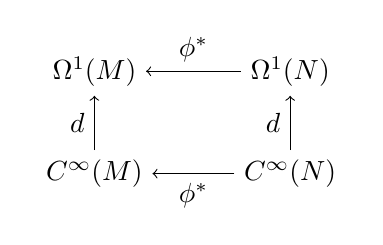
\begin{tikzpicture}
  \matrix (m) [matrix of math nodes, row sep=2em, column sep=3em, minimum width=1em]
  {
 \Omega^1(M)  &  \Omega^1(N)   \\
C^{\infty}(M) & C^{\infty}(N)  \\  };
%  \path[-stealth]
  \path[->]
  (m-1-2) edge node [above] {$\phi^*$} (m-1-1)
%  edge node [left] {$\text{ev}_0$} (m-2-2)
%  (m-1-1) edge node [left] {$\alpha$} (m-2-1)
  (m-2-2) edge node [auto] {$d$} (m-1-2)
%  edge node [below] {$\pi_M$} (m-2-2);
  edge node [auto] {$\phi^*$} (m-2-1)
  (m-2-1) edge node [left] {$d$} (m-1-1);
\end{tikzpicture}

\questionhead{}

\[
(\phi_*)^a_{ \, \, b} := (dy^a)(\phi_*( \frac{ \partial }{ \partial x^b } ) )
\]
\[
\text{ Let } g \in C^{\infty}(N)
\]
\[
\begin{gathered}
  \phi_* \left( \frac{ \partial }{ \partial x^b} \right) g = \frac{ \partial x^b} g\phi(p) = \frac{ \partial }{ \partial x^b} g\phi x^{-1}x(p) = \frac{ \partial }{ \partial x^b}(gyy^{-1}\phi x^{-1})(x) = \\
  = \frac{ \partial }{ \partial x^b}(gy^{-1}(y\phi x^{-1}(x(p))) ) = \left. \frac{ \partial g}{ \partial y}^b \right|_y \left. \frac{ \partial y^a}{ \partial x^b} \right|_x = \frac{ \partial y^a}{ \partial x^b} \frac{ \partial g}{ \partial y^a}
\end{gathered}
\]
Then 
\[
\phi_*\left( \frac{ \partial }{ \partial x^b} \right) = \frac{ \partial y^a}{ \partial x^b} \frac{ \partial }{ \partial y^a}
\]
and so 
\[
(\phi_*)^a_{ \, \, b} = \frac{ \partial y^a}{ \partial x^b}
\]

\questionhead{}

\exercisehead{3}\textbf{:Lie derivative-the pedestrian way}

\questionhead{} While it is true that $\forall \, p \in S^2$, for $x(p) = (\theta, \varphi)$, and $(yix^{-1})(\theta,\varphi) = (y^1,y^2,y^3) \in \mathbb{R}^3$ and that, at this point $p$, $(y^1)^2/a^2 + (y^2)^2/b^2 +(y^3)^2/c^3 = 1$, this doesn't imply (EY: 20150321 I think) that, globally, it's an ellipsoid (yet).  In the familiar charts given, \\
spherical chart $(U,x) \in \mathcal{A}$ and \\
$(\mathbb{R}^3, y=\text{id}_{\mathbb{R}^3}) \in \mathcal{B}$ \\
it looks like an ellipsoid, but change to another choice of charts, and it could look something very different.  

\questionhead{}

Equip $(\mathbb{R}^3, \mathcal{O}_{\text{st}}, \mathcal{B})$ with the Euclidean metric $g$, and pullback $g$.  

Note that the pullback of the inclusion from $\mathbb{R}^3$ onto $S^2$ for the Euclidean metric is the following:
\[
i^* g\left( \frac{ \partial }{ \partial \theta^i }, \frac{ \partial }{ \partial \theta^j} \right) = g\left( i_*\frac{ \partial }{ \partial \theta^i }, i_*\frac{ \partial }{ \partial \theta^j} \right) = g\left( \frac{ \partial x^a}{ \partial \theta^i} \frac{ \partial }{ \partial x^a} , \frac{ \partial x^b}{ \partial \theta^j} \frac{ \partial }{ \partial x^b } \right) = g_{ab} \frac{ \partial x^a}{ \partial \theta^i} \frac{ \partial x^b}{ \partial \theta^j} 
\]
With $g_{ab}=\delta_{ab}$, the usual Euclidean metric, this becomes the following:
\[
g^{\text{ellipsoid}}_{ij} = \frac{ \partial x^a}{ \partial \theta^i} \frac{ \partial x^a}{ \partial \theta^j} 
\]

At this point, one should get smart (we are in the 21st century) and use some sort of CAS (Computer Algebra System). I like Sage Math (version 6.4 as of 20150322).  I also like the Sage Manifolds package for Sage Math.  

I like Sage Math for the following reasons:
\begin{itemize}
\item Open source, so it’s open and freely available to anyone, which fits into my principle of making online education open and freely available to anyone, anytime
\item Sage Math structures everything in terms of Category Theory and Categories and Morphisms naturally correspond to Classes and Class methods or functions in Object-Oriented Programming in Python and they’ve written it that way
\end{itemize}
and I like Sage Manifolds for roughly the same reasons, as manifolds are fit into a category theory framework that’s written into the Python code.  e.g.

{\small \begin{verbatim}
sage: S2 = Manifold(2, 'S^2', r'\mathbb{S}^2', start_index=1) ; print S2
sage: print S2
2-dimensional manifold 'S^2'
sage: type(S2)
<class 'sage.geometry.manifolds.manifold.Manifold_with_category'>
\end{verbatim}}

With code (I’ve provided for convenience; you can make your own as I wrote it based upon to example of $S^2$ on the sagemanifolds documentation website page), load it and do the following:

cf. \url{https://github.com/ernestyalumni/diffgeo-by-sagemnfd/blob/master/S2.sage} \\
\url{http://sagemanifolds.obspm.fr/examples.html}

{\scriptsize \begin{verbatim}
sage: load("S2.sage")
sage: U_ep = S2.open_subset('U_{ep}')
sage: eps.<the,phi> = U_ep.chart()
sage: a = var(“a”)
sage: b = var(“b”)
sage: c = var("c")
sage: inclus = S2.diff_mapping(R3, {(eps, cart): [ a*cos(phi)*sin(the), b*sin(phi)*sin(the),c*cos(the) ]} , name="inc",latex_name=r'\mathcal{i}')
sage: inclus.pullback(h).display()
inc_*(h) = (c^2*sin(the)^2 + (a^2*cos(phi)^2 + b^2*sin(phi)^2)*cos(the)^2) dthe*dthe - (a^2 - b^2)*cos(phi)*cos(the)*sin(phi)*sin(the) dthe*dphi 
- (a^2 - b^2)*cos(phi)*cos(the)*sin(phi)*sin(the) dphi*dthe + (b^2*cos(phi)^2 + a^2*sin(phi)^2)*sin(the)^2 dphi*dphi
sage: inclus.pullback(h)[2,2].expr()
(b^2*cos(phi)^2 + a^2*sin(phi)^2)*sin(the)^2
\end{verbatim}
}
A new open subset $U_{\text{ep}}$ was declared in $S^2$, a new chart $(U_{\text{ep}}, (\theta,\phi))$ was declared, the constants, $a,b,c$, were declared, and the inclusion map given in the problem
\[
y\circ \mathfrak{i} \circ x^{-1} : (\theta, \phi) \mapsto ( a\cos{\phi} \sin{\theta}, b \sin{\phi} \sin{\theta}, c\cos{\theta})
\]
Then the pullback of the inclusion map $\mathcal{i}$ was done on the Euclidean metric $h$, defined earlier in the file \begin{verbatim}S2.sage\end{verbatim}.  Then one can access the components of this metric and do, for example, \begin{verbatim}simplify_full(),full_simplify(), reduce_trig()\end{verbatim} on the expression.  

In Python, I could easily do this, and give an answer quick in LaTeX:

%{\scriptsize 
\begin{verbatim}
sage: for i in range(1,3): 
....:     for j in range(1,3):
....:         print inclus.pullback(h)[i,j].expr()
....:         latex(inclus.pullback(h)[i,j].expr() )
....:         
c^2*sin(the)^2 + (a^2*cos(phi)^2 + b^2*sin(phi)^2)*cos(the)^2
\end{verbatim}
(EY: I'll suppress the LaTeX output but this sage math function gives you LaTeX code)
%c^{2} \sin\left(\mathit{the}\right)^{2} + {\left(a^{2} \cos\left(\phi\right)^{2} + 
%b^{2} \sin\left(\phi\right)^{2}\right)} \cos\left(\mathit{the}\right)^{2}
%-(a^2 - b^2)*cos(phi)*cos(the)*sin(phi)*sin(the)
%-{\left(a^{2} - b^{2}\right)} \cos\left(\phi\right) \cos\left(\mathit{the}\right) \sin\left(\phi\right) \sin\left(\mathit{the}\right)
%-(a^2 - b^2)*cos(phi)*cos(the)*sin(phi)*sin(the)
%-{\left(a^{2} - b^{2}\right)} \cos\left(\phi\right) \cos\left(\mathit{the}\right) \sin\left(\phi\right) \sin\left(\mathit{the}\right)
%(b^2*cos(phi)^2 + a^2*sin(phi)^2)*sin(the)^2
%{\left(b^{2} \cos\left(\phi\right)^{2} + a^{2} \sin\left(\phi\right)^{2}\right)} \sin\left(\mathit{the}\right)^{2}
%
%

and so

\[
\boxed{ \begin{gathered}
 i^* g = c^{2} \sin\left(\mathit{the}\right)^{2} + {\left(a^{2} \cos\left(\phi\right)^{2} + b^{2} \sin\left(\phi\right)^{2}\right)} \cos\left(\mathit{the}\right)^{2} d\theta \otimes d\theta + \\
-2 {\left(a^{2} - b^{2}\right)} \cos\left(\phi\right) \cos\left(\mathit{the}\right) \sin\left(\phi\right) \sin\left(\mathit{the}\right) d\theta \otimes d\phi +  \\
 + {\left(b^{2} \cos\left(\phi\right)^{2} + a^{2} \sin\left(\phi\right)^{2}\right)} \sin\left(\mathit{the}\right)^{2} d\phi \otimes d\phi 
\end{gathered} }
\]

\questionhead{}

{\small
\begin{verbatim}
sage: polar_vees = eps.frame()
sage: X_1 = - sin(phi) * polar_vees[1] - cot( the ) * cos(phi) * polar_vees[2]
sage: X_2 = cos( phi ) * polar_vees[1] - cot( the ) * sin( phi) * polar_vees[2]
sage: X_3 = polar_vees[2]
sage: X_2.lie_der(X_1).display()
(cos(the)^2 - 1)/sin(the)^2 d/dphi
sage: X_3.lie_der(X_1).display()
cos(phi) d/dthe - cos(the)*sin(phi)/sin(the) d/dphi
sage: X_3.lie_der(X_2).display()
sin(phi) d/dthe + cos(phi)*cos(the)/sin(the) d/dphi
\end{verbatim}
}

Indeed, one can check on a scalar field $f_{\text{eps}} \in C^{\infty}(S^2)$:
{\small
\begin{verbatim}
sage: f_eps = S2.scalar_field({eps: function('f', the, phi ) }, name='f' )
sage: (X_1( X_2(f_eps)) - X_2(X_1(f_eps) ) ).display()
U_{ep} --> R
(the, phi) |--> -D[1](f)(the, phi)
sage: X_2.lie_der(X_1) == -X_3
True
sage: X_3.lie_der(X_1) == X_2
True
sage: X_3.lie_der(X_2) == -X_1
True
\end{verbatim}
}

\[
\Longrightarrow \boxed{ [X_i, X_j] = -\epsilon_{ijk}X_k }
\]
So $\text{span}_{\mathbb{R}} \lbrace X_1,X_2,X_3 \rbrace$ equipped with $[ \, , \, ]$ constitute a Lie subalgebra on $S^2$ (It's closed under $[ \, , \, ]$

\section{Integration}

\subsection{}

\subsection{}

\subsection{Volume forms}

\begin{definition}
On a smooth manifold $(M,\mathcal{O},\mathcal{A})$ \\
a $(0,\text{dim}M)$-tensor field $\Omega$ is called a \underline{volume form} if 
\begin{enumerate}
\item[(a)] $\Omega$ vanishes nowhere (i.e. $\Omega \neq 0 \, \, \forall \, p \in M$) 
\item[(b)] totally antisymmetric 
\[
\Omega(\dots , \underbrace{X}_{i\text{th}} , \dots , \underbrace{Y}_{j\text{th}} \dots ) = - \Omega(\dots , \underbrace{Y}_{i\text{th}} , \dots , \underbrace{X}_{j\text{th}} \dots )
\]
\end{enumerate}

In a chart: 
\[
\Omega_{i_1 \dots i_d} = \Omega_{ [i_1 \dots i_d ]}
\]
\end{definition}

\underline{Example} $(M,\mathcal{O}, \mathcal{A},g)$ metric manifold

construct volume form $\Omega$ from $g$

In \underline{any} chart: $(U,x)$

\[
\Omega_{i_1 \dots i_d} := \sqrt{ \text{det}(g_{ij}(x)) } \epsilon_{i_1 \dots i_d} 
\]
where \textbf{Levi-Civita symbol} $\epsilon_{i_1 \dots i_d}$ is \underline{defined} as $\begin{aligned} & \quad \\ 
& \epsilon_{123 \dots d} = +1 \\ 
& \epsilon_{1\dots d} = \epsilon_{[i_1 \dots i_d]} \end{aligned}$

\begin{proof} (well-defined) Check: What happens under a change of charts
\[
\begin{aligned}
\Omega(y)_{i_1 \dots i_d} & = \sqrt{ \text{det}(g(y)_{ij}) } \epsilon_{i_1 \dots i_d} = \\
& = \sqrt{ \text{det}(g_{mn}(x) \frac{ \partial x^m}{ \partial y^i} \frac{ \partial x^n}{ \partial y^j} )} \frac{ \partial y^{m_1} }{ \partial x^{i_1} } \dots \frac{ \partial y^{m_d}}{ \partial x^{i_d}} \epsilon_{ [m_1 \dots m_d] } = \\
& = \sqrt{ | \text{det}g_{ij}(x) | } \left| \text{det}\left( \frac{ \partial x}{ \partial y} \right) \right| \text{det}\left( \frac{ \partial y}{ \partial x} \right) \epsilon_{i_1 \dots i_d} = \sqrt{ \text{det}g_{ij}(x)} \epsilon_{i_1 \dots i_d} \text{sgn}\left( \text{det}\left( \frac{ \partial x}{ \partial y} \right) \right)
\end{aligned}
\]
\end{proof}

EY : 20150323 

Consider the following:
\[
\begin{aligned}
\Omega(y)(Y_{(1)} \dots Y_{(d)} ) & = \Omega(y)_{i_1 \dots i_d}Y_{(1)}^{i_1} \dots Y_{(d)}^{i_d} =  \\
& = \sqrt{ \text{det}(g_{ij}(y)) } \epsilon_{i_1 \dots i_d} Y^{i_1}_{(1)} \dots Y^{i_d}_{(d)} = \\
& = \sqrt{ \text{det}(g_{mn}(x)) \frac{ \partial x^m}{ \partial y^i} \frac{ \partial x^n }{ \partial y^j} } \epsilon_{i_1 \dots i_d} \frac{ \partial y^{i_1}}{ \partial x^{m_1} } \dots \frac{ \partial y^{i_d} }{ \partial x^{m_d} } X^{m_1} \dots X^{m_d}  = \\
& = \sqrt{ \text{det}(g_{mn}(x))\frac{ \partial x^m}{ \partial y^i} \frac{ \partial x^n}{ \partial y^j}} \text{det}\left( \frac{ \partial y}{ \partial x}\right) \epsilon_{m_1 \dots m_d} X^{m_1} \dots X^{m_d} = \\
& = \sqrt{ \text{det}(g_{mn}(x)) } \left| \text{det}\left( \frac{ \partial x}{ \partial y} \right) \right| \text{det}\left( \frac{ \partial y}{ \partial x} \right) \epsilon_{m_1 \dots m_d} X^{m_1} \dots X^{m_d} = \\
& = \sqrt{\text{det}(g_{mn}(x))} \epsilon_{m_1 \dots m_d} \text{sgn}\left(\text{det}\left( \frac{ \partial x}{ \partial y} \right) \right) X^{m_1} \dots X^{m_d} = \text{sgn}(\text{det}\left( \frac{ \partial x}{ \partial y} \right)) \Omega_{m_1 \dots m_d}(x) X^{m_1} \dots X^{m_d}
\end{aligned}
\]

If $\text{det}\left( \frac{ \partial y}{ \partial x} \right) > 0$, 
\[
\Omega(y)(Y_{(1)} \dots Y_{(d)})  = \Omega(x)(X_{(1)} \dots X_{(d)} )
\]
This works also if Levi-Civita symbol $\epsilon_{i_1\dots i_d}$ doesn't change at all under a change of charts. (around 42:43 \url{https://youtu.be/2XpnbvPy-Zg})

\hrulefill

Alright, let's require, \\
\phantom{\quad \, } restrict the smooth atlas $\mathcal{A}$ \\
\phantom{\quad \quad \, } to a subatlas ($\mathcal{A}^{\uparrow}$ still an atlas) 
\[
\mathcal{A}^{\uparrow} \subseteq \mathcal{A}
\]
s.t. $\forall \, (U,x), (V,y)$ have chart transition maps $\begin{aligned} & \quad \\ 
& y\circ x^{-1} \\ 
& x\circ y^{-1} \end{aligned}$

s.t. $\text{det}\left( \frac{ \partial y}{ \partial x} \right) >0$  \\
\phantom{ \quad \, } such $\mathcal{A}^{\uparrow} $ called an \textbf{oriented} atlas 

\[
(M, \mathcal{O}, \mathcal{A},g) \Longrightarrow (M,\mathcal{O},\mathcal{A}^{\uparrow} ,g)
\]
Note: associated bundles.

Note also:
$ \text{det}\left( \frac{ \partial y^b}{ \partial x^a} \right) = \text{det}(\partial_a(y^bx^{-1}))$ \phantom{ \quad \quad \, } $\frac{ \partial y^b}{ \partial x^a}$ is an endomorphism on vector space $V$.  $\begin{aligned} & \quad \\ 
& \varphi : V \to V \\
& \text{det}\varphi \quad \, \text{ independent of choice of basis } \end{aligned}$

\phantom{\quad \quad \, } $g$ is a $(0,2)$ tensor field, not endomorphism (not independent of choice of basis) $\sqrt{ |\text{det}(g_{ij}(y)) | }$

\begin{definition} $\Omega$ be a volume form on $(M,\mathcal{O}, \mathcal{A}^{\uparrow} )$ and consider chart $(U,x)$ 
\begin{definition} $\omega_{(X)} := \Omega_{i_1\dots i_d} \epsilon^{i_1\dots i_d}$
same way $\begin{aligned} & \quad \\ 
& \epsilon^{12 \dots d} = +1 \\ 
& \epsilon^{[\dots ]} \end{aligned}$

one can show

\[
\boxed{ \omega_{(y)} = \text{det}\left( \frac{ \partial x}{ \partial y} \right) \omega_{(x)} } \quad \quad \, \text{ scalar density }
\]
\end{definition}
\end{definition}

\subsection{Integration on \underline{one} chart domain $U$}

\begin{definition}
\begin{equation}
\boxed{ \int_U f :\overset{ (U,y) }{=} \int_{y(U)} d^d\beta \omega_{(y)}(y^{-1}(\beta)) f_{(y)}(\beta) }
\end{equation}
\end{definition}

\begin{proof}: Check that it's (well-defined), how it changes under change of charts
\[
\begin{gathered}
\int_U f :\overset{ (U,y) }{=} \int_{y(U)} d^d\beta \omega_{(y)}(y^{-1}(\beta)) f_{(y)}(\beta) = \underset{ (U,y)}{=} \int_{x(U)} \int d^d\alpha \left| \text{det}\left( \frac{ \partial y }{ \partial x}\right) \right| f_{(x)}(\alpha) \omega_{(x)}(x^{-1}(\alpha) \text{det}\left( \frac{ \partial x}{ \partial y } \right) = \\
= \int_{x(U)} d^d \alpha \omega_{(x)}(x^{-1}(x)) f_{(x)}(\alpha)
\end{gathered}
\]
\end{proof}

On an oriented metric manifold $(M,\mathcal{O}, \mathcal{A}^{\uparrow}, g)$
\[
\int_Uf:= \int_{x(U)} d^d\alpha  \underbrace{  \sqrt{ \text{det}(g_{ij}(x))(x^{-1}(\alpha)) } }_{\sqrt{g}}  f_{(x)}(\alpha)
\]

\subsection{Integration on the entire manifold}

\section{Lecture 13: Relativistic spacetime}

Recall, from Lecture 9, the definition of Newtonian spacetime
\[
(M, \mathcal{O}, \mathcal{A}, \nabla, t) \quad \quad \quad \, \begin{aligned}
& \nabla \text{ torsion free } \\
& t \in C^{\infty}(M) \\ 
& dt \neq 0 \\
& \nabla dt = 0   \quad \, \text{ (uniform time) }
\end{aligned}
\]
and the definition of relativistic spacetime (before Lecture )


\[
(M, \mathcal{O}, \mathcal{A}^{\uparrow}, \nabla, g, T ) \quad \quad \quad \, \begin{aligned}
& \nabla \text{ torsion-free } \\
& g \text{ Lorentzian metric} (+---) \\ 
& T \text{ time-orientation }
\end{aligned}
\]

\subsection{Time orientation}

\begin{definition}
  $(M,\mathcal{O},\mathcal{A}^{\uparrow},g)$ a Lorentzian manifold.  Then a time-orientation is given by a vector field $T$ that 
\begin{enumerate}
\item[(i)] does \textbf{not} vanish anywhere 
\item[(ii)] $g(T,T)>0$
\end{enumerate}
\end{definition}

Newtonian vs. relativistic \\
Newtonian \\
$X$ was called future-directed if 
\[
dt(X) >0
\]
$\forall \, p \in M$, take half plane, half space of $T_pM$ \\
also stratified atlas so make planes of constant $t$ straight \\
relativistic \\
half cone $\forall \, p, q \in M$, half-cone $\subseteq T_pM$ \\

This definition of \underline{spacetime}

Question \\
I see how the cone structure arises from the new metric. I don't understand however, how the $T$, the time orientation, comes in \\

Answer \\
$(M,\mathcal{O}, \mathcal{A},g)$ $g \xleftarrow (+---)$

requiring $g(X,X)>0$, select cones \\
$T$ chooses which cone \\

This definition of \underline{spacetime} has been made to enable the following physical postulates:
\begin{enumerate}
\item[(P1)] The worldline $\gamma$ of a \underline{massive} particle satisfies
\begin{enumerate}
  \item[(i)] $g_{\gamma(\lambda)}(v_{\gamma, \gamma(lambda)} , v_{\gamma,\gamma(\lambda)} ) >0$
  \item[(ii)] $g_{\gamma(\lambda)}(T, v_{\gamma,\gamma(\lambda)}) >0$
\end{enumerate}
\item[(P2)] Worldlines of \underline{massless} particles satisfy
\begin{enumerate}
\item[(i)] $g_{\gamma(\lambda)}(v_{\gamma,\gamma(\lambda)}, v_{\gamma,\gamma(\lambda)}) = 0$
\item[(ii)] $g_{\gamma(\lambda)}(T,v_{\gamma,\gamma(\lambda)}) >0$
\end{enumerate}
\underline{picture}: spacetime:
\end{enumerate}

Answer (to a question) $T$ is a smooth vector field, $T$ determines future vs. past, ``general relativity: we have such a time orientation; smoothness makes it less arbitrary than it seems'' -FSchuller,


\underline{Claim}: $9/10$ of a metric are determined by the cone

spacetime determined by distribution, only one-tenth error 

\subsection{Observers} $(M,\mathcal{O}, \mathcal{A}^{\uparrow},\nabla ,g, T)$
\begin{definition}
  An \underline{observer} is a worldline $\gamma$ with
\[
\begin{aligned}
  & g(v_{\gamma}, v_{\gamma}) >  0 \\ 
  & g(T,v_{\gamma}) > 0 
\end{aligned}
\]
together with a choice of basis
\[
v_{\gamma,\gamma(\lambda)} \equiv e_0(\lambda) , e_1(\lambda), e_2(\lambda), e_3(\lambda)
\]
of each $T_{\gamma(\lambda)}M$ where the observer worldline passes, if $g(e_a(\lambda), e_b(\lambda)) = \eta_{ab} = \left[ \begin{matrix} 1 & & & \\ & -1 & & \\ & & -1 & \\ & & & -1 \end{matrix} \right]_{ab}$

\underline{precise}: observer $=$ \underline{smooth} curve in the frame bundle $LM$ over $M$
\end{definition}

\subsubsection{Two physical postulates}

\begin{enumerate}
  \item[(P3)] A \textbf{clock} carried by a specific observer $(\gamma, e)$ will measure a \textbf{time}
\[
\tau := \int_{\lambda_0}^{\lambda_1} d\lambda \sqrt{ g_{\gamma(\lambda)}(v_{\gamma,\gamma(\lambda)}, v_{\gamma,\gamma(\lambda)}) }
\]
between the two ``\underline{events}''
\[
\gamma(\lambda_0) \quad \quad \quad \, \text{ ``start the clock'' }
\]
and 
\[
\gamma(\lambda_1) \quad \quad \quad \, \text{ ``stop the clock'' }
\]
\underline{Compare} with Newtonian spacetime:
\[
t(p)=7
\]

Thought bubble: \underline{proper time/eigentime} $\tau$

\underline{Application/Example.}
$\begin{aligned}
& M = \mathbb{R}^4 \\ 
 & \mathcal{O} = \mathcal{O}_{\text{st}} \\
  & \mathcal{A} \ni (\mathbb{R}^4, \text{id}_{\mathbb{R}^4} ) \\ 
  & g : g_{(x)ij} = \eta_{ij} \quad \, ; \quad \quad \, T_{(x)}^i =(1,0,0,0)^i
\end{aligned}
$
\[
\Longrightarrow \Gamma_{(x) \, \, jk }^i = 0 \text{ everywhere }
\]
$\Longrightarrow (M,\mathcal{O}, \mathcal{A}^{\uparrow},g,T,\nabla)$ \quad \, $\text{Riemm}=0$ \\
$\Longrightarrow $ spacetime is flat

This situation is called special relativity.

Consider two observers: 
\[
\begin{aligned} & 
\begin{aligned}
& \gamma : (0,1) \to M \\ 
 & \gamma_{(x)}^i = (\lambda , 0 ,0  ,0 )^i \end{aligned} \\
& 
\begin{aligned}
  & \delta :(0,1) \to M \\
\alpha \in (0,1) :   & \delta_{(x)}^i = \begin{cases} ( \lambda , \alpha \lambda , 0 , 0)^i & \lambda \leq \frac{1}{2} \\ 
    (\lambda, (1-\lambda)\alpha, 0,0)^i & \lambda > \frac{1}{2} \end{cases}
\end{aligned}
\end{aligned}
\]
let's calculate:
\[
\begin{aligned}
  & \tau_{\gamma}:= \int_0^1 \sqrt{ g_{(x)ij} \dot{\gamma}^i_{(x)} \dot{\gamma}^j_{(x)} } = \int_0^1 d\lambda 1 = 1 \\
  & \tau_{\delta} := \int_0^{1/2} d\lambda \sqrt{ 1- \alpha^2} + \int_{1/2}^1 \sqrt{ 1^2 - (-\alpha)^2 } = \int_0^1 \sqrt{ 1 - \alpha^2 } = \sqrt{ 1 - \alpha^2}
\end{aligned}
\]
Note: piecewise integration

Taking the clock postulate (P3) seriously, one better come up with a realistic clock design that supports the postulate. 
\underline{idea}.

2 little mirrors
\item[(P4)] \underline{Postulate}

Let $(\gamma, e)$ be an observer, and \\
$\delta$ be a \emph{massive} particle worldline that is parametrized s.t. $g(v_{\gamma}, v_{\gamma})=1$ (for parametrization/normalization convenience)

Suppose the observer and the particle \emph{meet} somewhere (in spacetime)
\[
\delta(\tau_2) = p = \gamma(\tau_1)
\]

\emph{This} observer measures the 3-velocity (spatial velocity) of this particle as 
\begin{equation}\label{Eq:spatialv}
v_{\delta}: \epsilon^{\alpha}( v_{\delta, \delta(\tau_2)} ) e_{\alpha} \quad \quad \quad \, \alpha =1,2,3
\end{equation}
where $\epsilon^0, \boxed{ \epsilon^1,\epsilon^2,\epsilon^3}$ is the unique dual basis of $e_0,\boxed{ e_1,e_2,e_3}$
\end{enumerate}

EY:20150407

There might be a major correction to Eq. (\ref{Eq:spatialv}) from the Tutorial 14 : Relativistic spacetime, matter, and Gravitation, see the second exercise, Exercise 2, third question:
\begin{equation}
v := \frac{ \epsilon^{\alpha}({v}_{\delta} ) }{ \epsilon^0({v}_{\delta}) } e_{\alpha}
\end{equation}

\underline{Consequence}:
An observer $(\gamma, e)$ will extract quantities measurable in his laboratory from objective spacetime quantities always like that.

\underline{Ex}: $F$ Faraday $(0,2)$-tensor of electromagnetism:

\[
F(e_a,e_b) = F_{ab} = \left[ \begin{matrix} 0 & E_1 & E_2 & E_3 \\ 
    -E_1 & 0 & B_3 & -B_2 \\ 
    -E_2 & -B_3 & 0 & B_1 \\
    -E_3 & B_2 & -B_1 & 0 \end{matrix} \right]
\]
observer frame $e_a,e_b$

$E_{\alpha} := F(e_0,e_{\alpha})$ \\
$B^{\gamma}:= F(e_{\alpha},e_{\rho})\epsilon^{\alpha \beta \gamma}$
where 
$\epsilon^{123} = +1$ totally antisymmetric

\subsection{Role of the Lorentz transformations}

Lorentz transformations emerge as follows: \\
Let $(\gamma,e)$ and $(\widetilde{\gamma},\widetilde{e})$ be observers with $\gamma(\tau_1) = \widetilde{\gamma}(\tau_2)$

(for simplicity $\gamma(0) = \widetilde{\gamma}(0)$

Now 
\[
\begin{gathered}
  e_0 , \dots , e_1 \quad \quad \quad \, \text{ at } \tau = 0 \\
  \text{ and } 
  \widetilde{e}_0 , \dots , \widetilde{e}_1 \quad \quad \quad \, \text{ at }  \tau = 0 \\
\end{gathered}
\]
both bases for the same $T_{\gamma(0)}M$

\underline{Thus}: $\widetilde{e}_a = \Lambda^b_{ \, \, a} e_b $ \quad \quad \, $\Lambda \in GL(4)$

Now:

\[
\begin{aligned}
  \eta_{ab} = g(\widetilde{e}_a, \widetilde{e}_b) & = g(\Lambda^m_{ \, \, a}e_m, \Lambda^n_{ \, \, b} e_n ) = \\
  & = \Lambda^m_{ \, \, a} \Lambda^n_{ \, \, b} \underbrace{g(e_m,e_n)}_{ \eta_{mn}}
\end{aligned}
\]
i.e. $\Lambda \in O(1,3)$

\underline{Result}: Lorentz transformations relate the \emph{frames} of \emph{any two observers} at the same point.

``$\widetilde{x}^{\mu} - \Lambda^{\mu}_{ \, \, \nu} x^{\nu}$'' is utter nonsense

\subsection*{Tutorial}

I didn't see a tutorial video for this lecture, but I saw that the Tutorial sheet number 14 had the relevant topics.  Go there.

\section{Lecture 14: \underline{Matter}}

two types of matter

point matter

\underline{field matter}

\underline{point matter}

massive point particle 

more of a phenomenological importance

\underline{field matter}
 
electromagnetic field

more fundamental from the GR point of view


both classical matter types


\subsection{Point matter}

Our postulates (P1) and (P2) already constrain the possible particle worldlines.  

But what is their precise law of motion, possibly in the presence of ``forces'',

\begin{enumerate}
\item[(a)] \underline{without external forces}
\[
S_{\text{massive}}[\gamma] := m \int d\lambda \sqrt{ g_{\gamma(\lambda)}( v_{\gamma,\gamma(\lambda)} , v_{\gamma,\gamma(\lambda) } ) }
\]
\underline{with}:
\[
g_{\gamma(\lambda)}(T_{\gamma(\lambda)}, v_{\gamma, \gamma(\lambda) } ) > 0 
\]
dynamical law Euler-Lagrange equation

\underline{similarly}
\[
S_{\text{massless}}[\gamma,\mu] = \int d\lambda \mu g(v_{\gamma, \gamma(\lambda)} , v_{\gamma,\gamma(\lambda)} )
\]
\[
\begin{aligned}
  \delta_{\mu}  \quad \quad \, & g(v_{\gamma,\gamma(\lambda)}, v_{\gamma,\gamma(\lambda) } ) = 0 \\
 \delta_{\gamma} \quad \quad \, & \text{e.o.m.}
\end{aligned}
\]

Reason for describing equations of motion by actions is that composite systems have an action that is the sum of the actions of the parts of that system, possibly including ``\underline{interaction terms.}''

\underline{Example}. \[
S[\gamma] + S[\delta] + S_{\text{int}}[\gamma,\delta]
\]
\item[(b)] \underline{presence of external forces} \\
or rather presence of \underline{fields} to which a particle ``\underline{couples}''

\underline{Example}
\[
S[\gamma;A] = \int d\lambda m \sqrt{ g_{\gamma(\lambda)}(v_{\gamma, \gamma(\lambda)}, v_{\gamma,\gamma(\lambda)} ) } + qA(v_{\gamma,\gamma(\lambda)})
\]
where $A$ is a \textbf{covector field} on $M$. $A$ fixed
(e.g. the electromagnetic potential)
\end{enumerate}

Consider Euler-Lagrange eqns. $L_{\text{int}} = q A_{(x)} \dot{\gamma}^m_{(x)}$
\[
m (\nabla_{v_{\gamma}} v_{\gamma})_a + \underbrace{ \dot{ \left( \frac{ \partial L_{\text{int}} }{ \partial \dot{\gamma}^m_{(x)} } \right) }- \frac{ \partial L_{\text{int}} }{ \partial \gamma^m_{(x)} } }_{*} = 0  \Longrightarrow \boxed{ m (\nabla_{v_{\gamma} } v_{\gamma})^a = \underbrace{ -q F^a_{ \, \, m } \dot{\gamma}^m }_{\text{Lorentz force on a charged particle in an electromagnetic field } } }
\]
\[
\frac{ \partial L}{ \partial \dot{\gamma}^a} = qA_{(x)a}, \quad \quad \, \dot{ \left( \frac{ \partial L}{ \partial \dot{\gamma}^m} \right) } = q \cdot \frac{ \partial }{ \partial x^m} (A_{(x)m} ) \cdot \dot{\gamma}^m_{(x)}
\]
\[
\frac{ \partial L}{ \partial \gamma^a} = q \cdot \frac{ \partial }{ \partial x^a} (A_{(x)m} ) \dot{\gamma}^m
\]
\[
\begin{aligned}
* & = q\left( \frac{ \partial A_a}{ \partial x^m} - \frac{ \partial A_m}{ \partial x^a} \right) \dot{\gamma}^m_{(x)}
& = q \cdot F_{(x)am} \dot{\gamma}^m_{(x)}
\end{aligned}
\]
$F \leftarrow $ Faraday

\[
S[\gamma] = \int(m\sqrt{g(v_{\gamma},v_{\gamma} ) } + q A(v_{\gamma}) ) d\lambda
\]

\subsection{Field matter}

\begin{definition}
  Classical (non-quantum) field matter is any tensor field on spacetime where equations of motion derive from an action.
\end{definition}

\underline{Example}: 
\[
S_{\text{Maxwell}}[A] = \frac{1}{4}\int_M d^4x \sqrt{-g}F_{ab}F_{cd}g^{ac}g^{bd}
\]
$A$ $(0,1)$-tensor field \\
$=$ thought cloud: for \underline{simplicity} one chart covers all of $M$ \\
$-$ for $\sqrt{-g}$ $(+---)$ \\

$F_{ab} := 2\partial_{[a}A_{b]} = 2(\nabla_{[a} A)_{b]}$

\underline{Euler-Lagrange equations for fields}
\[
0 = \frac{ \partial \mathcal{L}}{ \partial A_m} - \frac{ \partial }{ \partial x^s} \left( \frac{ \partial \mathcal{L}}{ \partial \partial _s A_m } \right) + \frac{ \partial }{ \partial x^s} \frac{ \partial }{ \partial x^t} \frac{ \partial^2 \mathcal{L}}{ \partial \partial_t \partial_s A_m }
\]

\underline{Example} \dots 
\[
(\nabla_{\frac{ \partial }{ \partial x^m} }F)^{ma} = j^a
\]
\textbf{in}homogeneous Maxwell

thought bubble $j=qv_{\gamma}$

\[
\partial_{[a}F_{b]} - ()
\]
homogeneous Maxwell

Other example well-liked by textbooks
\[
S_{\text{Klein-Gordon}}[\phi] := \int_M d^4x \sqrt{-g}[g^{ab}(\partial_a \phi) (\partial_b \phi ) - m^2\phi^2]
\]
$\phi$ $(0,0)$-tensor field

\subsection{Energy-momentum tensor of matter fields}

At some point, we want to write down an \underline{action} for the metric tensor field itself.

But then, this action $S_{\text{grav}}[g]$ will be added to any $S_{\text{matter}}[A,\phi,\dots]$ in order to describe the total system.  

\[
S_{\text{total}}[g,A] = S_{\text{grav}}[g] + S_{\text{Maxwell}}[A,g]
\]

\[
\begin{aligned}
  & \delta A     & : \Longrightarrow \text{ Maxwell's equations } \\
  & \delta g_{ab} & : \boxed{ \frac{1}{ 16 \pi G } G^{ab} } + (-2T^{ab} ) = 0 
\end{aligned}
\]
$G$ Newton's constant

\[
G^{ab} = 8 \pi G_N T^{ab}
\]

\begin{definition}
$  S_{\text{matter}}[\Phi,g] $ is a matter action, the \textbf{so-called energy-momentum tensor} is 
\[
T^{ab} := \frac{-2}{ \sqrt{-g}} \left( \frac{ \partial \mathcal{L}_{\text{matter}} }{ \partial g_{ab}} - \partial_s \frac{ \partial \mathcal{L}_{\text{matter}} }{ \partial \partial_s g_{ab}} + \dots \right)
\]
\end{definition}
$-$ of $\frac{-2}{\sqrt{g}}$ is Schr\"{o}dinger minus (EY : 20150408 F.Schuller's joke? but wise)

choose all sign conventions s.t.
\[
T(\epsilon^0,\epsilon^0) >0
\]

\underline{Example}: For $S_{\text{Maxwell}}$:
\[
T_{ab} = F_{am} F_{bn}g^{mn} - \frac{1}{4} F_{mn} F^{mn} g_{ab}
\]
$T_{ab} \equiv T_{\text{Maxwell}ab}$

\[
T(e_0,e_0) = \underline{E}^2+\underline{B}^2
\]
\[
T(e_0,e_{\alpha}) = (E\times B)_{\alpha}
\]

\underline{Fact}: One often does not specify the fundamental action for some matter, but one is rather satisfied to assume certain properties / forms of 
\[
T_{ab}
\]

\underline{Example} Cosmology: (homogeneous \& isotropic)

perfect fluid \\

of pressure $p$ and density $\rho$
modelled by
\[
T^{ab} = (\rho + p)u^a u^b - pg^{ab}
\]

radiative fluid

What is a fluid of photons:

observe: $\begin{aligned}
  & T_{\text{Maxwell}}^{ \, \, ab} g_{ab} = 0 \\ 
  & T_{\text{p.f.}}^{ \, \, ab} g_{ab} \overset{!}{=} 0 \\
& = (\rho + p)u^a u^b g_{ab} - p\underbrace{ g^{ab} g_{ab} }_{ 4}
\end{aligned}$

\[
\begin{aligned}
 \leftrightarrow & \rho _ p 04p = 0 \\ 
 & \rho = 3p
\end{aligned}
\]
$p=\frac{1}{3}\rho$

Reconvene at 3 pm?  (EY : 20150409 I sent a Facebook (FB) message to the International Winter School on Gravity and Light: there was no missing video; it continues on Lecture 15 immediately)

\subsection*{Tutorial 14: Relativistic Spacetime, Matter and Gravitation}

\exercisehead{2: Lorentz force law}

\questionhead{electromagnetic potential}





\section{Lecture 15: Einstein gravity}

Recall that in Newtonian spacetime, we were able to reformulate the Poisson law $\Delta \phi = 4\pi G_N \rho$ in terms of the Newtonian spacetime curvature as 

\[
R_{00} = 4\pi G_N \rho
\]
$R_{00}$ with respect to $\nabla_{\text{Newton}}$

$G_N = $ Newtonian gravitational constant

This prompted Einstein to postulate $<$ 1915 that the relativistic field equations for the Lorentzian metric $g$ of (relativistic) spacetime
\[
R_{ab} = 8\pi G_N T_{ab} \cancel{ \quad }
\]

However, this equation suffers from a problem

LHS:
$(\nabla_a R)^{ab} \neq 0$ \\
generically

RHS:
\[
(\nabla_a T)^{ab}  = 0
\]
thought bubble: $=$ formulated from an action

Einstein tried to argue this problem away.  

Nevertheless, the equations cannot be upheld. 

\subsection{Hilbert}

Hilbert was a specialist for variational principles. 

To find the appropriate left hand side of the gravitational field equations, Hibert suggested to start from an action
\[
S_{\text{Hilbert}}[g] = \int_M \sqrt{-g} R_{ab}g^{ab}
\]
thought bubble $=$ ``simplest action''

\underline{aim}: varying this w.r.t. metric $g_{ab}$ will result in some tensor 
\[
G^{ab} = 0
\]

\subsection{Variation of $S_{\text{Hilbert}}$}

\[
\begin{gathered}
  0 \overset{!}{=} \underbrace{\delta}_{g_i} S_{\text{Hilbert}}[g] = \int_M [ \underbrace{ \delta \sqrt{-g} g^{ab}R_{ab} }_{1} + \underbrace{ \sqrt{-g} \delta g^{ab} R_{ab}}_{2} + \underbrace{ \sqrt{-g} g^{ab} \delta R_{ab} }_{3} ] 
\end{gathered}
\]
\[
\text{ and 1 : } \delta \sqrt{-g} = \frac{ - (\text{det}g)g^{mn} \delta g_{mn} }{ 2 \sqrt{-g}} = \frac{1}{2} \sqrt{-g} g^{mn} \delta g_{mn}
\]
thought bubble
\[
\begin{gathered}
  \delta \text{det}(g) = \text{det}(g) g^{mn} \delta g_{mn} \\ 
  \text{ e.g. from } \\
\text{det}(g) = \exp{ \text{tr}{ \ln{g} } }
\end{gathered}
\]

ad 2: $g^{ab}g_{bc} = \delta^a_c$
\[
\begin{gathered}
\Longrightarrow (\delta g^{ab})g_{bc} + g^{ab}(\delta g_{bc}) = 0  \\
 \Longrightarrow \delta g^{ab} = -g^{am} g^{bn} \delta g_{mn}
\end{gathered}
\]

ad 3: 
\[
\begin{gathered}
  \Delta R_{ab} \underbrace{=}_{\text{normal coords at point}} \delta \partial_b \Gamma^m_{ \, \, am} - \delta \partial_m \Gamma^m_{ \, \, ab} + \Gamma \Gamma - \Gamma \Gamma = \\
  \begin{aligned}
    & = \partial_b \delta \Gamma^m_{ \, \, am} - \partial_m \delta \Gamma^m_{ \, \, ab } = \\  
    & = \nabla_b (\delta \Gamma)^m_{ \, \, am} - \nabla_m (\delta \Gamma)^m_{ \, \, ab}
\end{aligned} \\
\Longrightarrow \sqrt{-g} g^{ab} \delta R_{ab} = \sqrt{-g}
\end{gathered}
\]
``if you formulate the variation properly, you'll see the variation $\delta$ commute with $\partial _b$'' EY : 20150408 I think one uses the integration at the bounds, integration by parts trick

$\Gamma^i_{(x) \, \, jk } - \widetilde{\Gamma}^i_{ (x) \, \, jk }$ are the components of a $(1,2)$-tensor.

Notation: $(\nabla_b A)^i_{ \, \, g} =: A^i_{ \, \, j;b}$

\[
\begin{gathered}
\Longrightarrow \sqrt{-g} g^{ab} \delta R_{ab}  \\
\underbrace{=}_{ \nabla g = 0 } \sqrt{-g} (g^{ab} \delta \Gamma^m_{ \, \, am} )_{;b} - \sqrt{-g} (g^{ab} \delta \Gamma^m_{ \, \, ab} )_{ ; m} = \sqrt{-g} A^b_{ \, \, ; b} - \sqrt{-g} B^m_{ \, \, , m }
\end{gathered}
\]

Question: Why is the difference of coefficients a tensor?

Answer:
\[
\begin{aligned}
\Gamma_{(y) \, \, jk}^i = \frac{ \partial y^i}{ \partial x^m} \frac{ \partial x^m}{ \partial y^j} \frac{ \partial x^q}{ \partial y^k} \Gamma^m_{(x) \,\ , nq} + \frac{ \partial y^i}{ \partial x^m} \frac{ \partial^2 x^m}{ \partial y^j \partial y^k}
\end{aligned}
\]

Collecting terms, one obtains

\[
\begin{aligned}
  0 & \overset{!}{=} \delta S_{\text{Hilbert}} = \int_M [ \frac{1}{2} \sqrt{-g} g^{mn} \delta g_{mn} g^{ab} R_{ab} - \sqrt{-g} g^{am} g^{bn} \delta g_{mn} R_{ab}+    \underbrace{ (\sqrt{-g}A^a)_{ \, , a} }_{ \text{surface} } - \underbrace{ ( \sqrt{-g} B^b)_{ \, , b } }_{ \text{surface term } } ] \\
  & = \int_M \sqrt{-g} \delta \underbrace{g_{mn}}_{ \text{arbitrary variation}} [ \frac{1}{2} g^{mn} R - R^{mn} ] \Longrightarrow G^{mn} = R^{mn} - \frac{1}{2} g^{mn} R
\end{aligned}
\]

Hence Hilbert, from this ``mathematical'' argument, concluded that one may take
\[
\begin{gathered}
\boxed{ R_{ab} - \frac{1}{2} g_{ab} R = 8 \pi G_N T_{ab} }  \\
 \text{ Einstein equations}
\end{gathered}
\]
\[
S_{E-H}[g] = \int_M \sqrt{-g}R
\]

\subsection{3. Solution of the $\nabla_a T^{ab} =0$ issue}

One can show ($\to$ Tutorials) that the \underline{Einstein curvature}
\[
G_{ab} = R_{ab} - \frac{1}{2} g_{ab}R
\]
satisfy the so-called \underline{contracted} \underline{differential Bianchi identity}
\[
(\nabla_a G)^{ab} =0 
\]

\subsection{Variants of the field equations}

\begin{enumerate}
\item[(a)] a simple rewriting:
\[
R_{ab} - \frac{1}{2} g_{ab} R = 8 \pi G_N T_{ab} = T_{ab}
\]
$G_N = \frac{1}{8\pi}$

Contract on both sides $g^{ab}$

\[
\begin{gathered}
\begin{aligned}
  & R_{ab} - \frac{1}{2} g_{ab} R = T_{ab} || g^{ab} \\ 
  & R - 2R = T := T_{ab}g^{ab}
\end{aligned} \\
\Longrightarrow R = -T
\end{gathered}
\]
\[
\begin{gathered}
\Longrightarrow R_{ab} + \frac{1}{2} g_{ab} T = T_{ab} \\
\Longleftrightarrow R_{ab} = (T_{ab} - \frac{1}{2} Tg_{ab}) =: \widehat{T}_{ab}
\end{gathered}
\]
\[
\boxed{ R_{ab} = \widehat{T}_{ab}}
\]

\item[(b)] \[
S_{E-H}[g] := \int_M \sqrt{-g} (R+ 2\Lambda)
\]
thought bubble: $\Lambda$ cosmological constant

\underline{History:}

1915: $\Lambda < 0$ (Einstein) in order to get a non-expanding universe

$>$1915: $\Lambda =0$ Hubble 

today $\Lambda > 0$ to account for an accelerated expansion

$\Lambda \neq 0$ can be interpreted as a contribution

$-\frac{1}{2} \Lambda g$ to the energy-momentum 

``dark energy''

Question: surface terms scalar?

Answer: for a careful treatment of the surface terms which we discarded, see, e.g. E. Poisson, ``A relativist's toolkit'' C.U.P. ``excellent book''

Question: What is a constant on a manifold?

Answer: $\int \sqrt{-g} \Lambda = \Lambda \int \sqrt{-g} 1$

[back to dark energy]

[Weinberg, QCD, calculated] \\
\underline{idea}: 1 could arise as the vacuum energy of the standard model fields 

$\Lambda_{\text{calculated}} = 10^{120} \times \Lambda_{\text{obs}}$

``worst prediction of physics''

\underline{Tutorials}: \underline{check that }
\begin{itemize}
\item Schwarzscheld metric (1916)
\item FRW metric 
\item pp-wave metric 
\item Reisner-Nordstrom 
\end{itemize}
$\Longrightarrow $ are solutions to Einstein's equations
\end{enumerate}

in high school 

$m\ddot{x} + m\omega^2 x^2=0$

$x(t) = \cos{(\omega t)}$

\underline{ET}: [elementary tutorials]

study motion of particles \& observers in Schwarzscheld S.T.

\underline{Satellite}: Marcus C. Werner

Gravitational lensing

odd number of pictures Morse theory (EY:20150408 Morse Theory !!!)

\underline{Domenico Giulini}

Hamiltonian form
Canonical Formulations

Key to Quantum Gravity


\section*{Tutorial 13 Schwarzschild Spacetime}

EY : 20150408 I'm not sure which tutorial follows which lecture at this point.

The tutorial video is excellent itself.  Here, I want to encourage the use of CAS to do calculations.  There are many out there.  Again, I'm partial to the Sage Manifolds package for Sage Math which are both open-source and based on Python. I'll use that here.  

\exercisehead{1} \textbf{Geodesics in a Schwarzschild spacetime}

\questionhead{Write down the Lagrangian}

Load ``Schwarzschild.sage'' in Sage Math, which will always be available freely here \url{https://github.com/ernestyalumni/diffgeo-by-sagemnfd/blob/master/Schwarzschild.sage}:

{\scriptsize
\begin{verbatim}
sage: load("Schwarzschild.sage")
4-dimensional manifold 'M'
open subset 'U_sph' of the 4-dimensional manifold 'M'
Levi-Civita connection 'nabla_g' associated with the Lorentzian metric 'g' on the 4-dimensional manifold 'M'
\end{verbatim}}
and so on.

Look at the code and I had defined the Lagrangian to be \begin{verbatim}L\end{verbatim}.  To get out the coefficients of $L$ of the components of the tangent vectors to the curve, i.e. $t', r',\theta',\phi'$, denoted \begin{verbatim}tp,rp,thp,php\end{verbatim} in my .sage file, do the following:

\begin{verbatim}
sage: L.expr().coefficients(tp)[1][0].factor().full_simplify()
(2*G_N*M_0 - r)/r
sage: L.expr().coefficients(rp)[1][0].factor().full_simplify()
-r/(2*G_N*M_0 - r)
sage: L.expr().coefficients(php)[1][0].factor().full_simplify()
r^2
sage: L.expr().coefficients(thp)[1][0].factor().full_simplify()
r^2*sin(th)^2
\end{verbatim}

\questionhead{There are 4 Euler-Lagrange equations for this Lagrangian. Derive the one with respect to the function $t(\lambda)$!}

\begin{verbatim}
sage: L.expr().diff(t)
0
\end{verbatim}
This confirms that $\frac{ \partial L}{ \partial t} =0$

For $\frac{d}{d\lambda} \frac{ \partial L}{ \partial t'}$, then one needs to consider this particular workaround for Sage Math (computer technicality).  One takes derivatives with respect to declared variables (declared with var) and then substitute in functions that are dependent upon $\lambda$, and then take the derivative with respect to the parameter $\lambda$.  This does that:

{\scriptsize
\begin{verbatim}
sage: L.expr().diff( thp ).factor().subs( r == gamma1 ).subs( thp == gamma3.diff( tau ) ).subs( th == gamma3 ).diff(tau)\
....: .factor()
2*(2*cos(gamma3(tau))*gamma1(tau)*D[0](gamma3)(tau)^2 + 2*sin(gamma3(tau))*D[0](gamma1)(tau)*D[0](gamma3)(tau) 
+ gamma1(tau)*sin(gamma3(tau))*D[0, 0](gamma3)(tau))*gamma1(tau)*sin(gamma3(tau))
\end{verbatim} }

\questionhead{Show that the Lie derivative of $g$ with respect to the vector fields $K_t :=\frac{\partial}{\partial t}$}

The first line defines the vector field by accessing the frame defined on a chart with spherical coordinates and getting the time vector.  The second line is the Lie derivative of $g$ with respect to this vector field.
\begin{verbatim}
sage: K_t = espher[0]
sage: g.lie_der(K_t).display() # 0, as desired
0
\end{verbatim}

EY : 20150410 My question is this: $\forall \, X \in \Gamma(TM)$ i.e. $X$ is a vector field on $M$, or, specifically, a section of the tangent bundle, then does
\[
\mathcal{L}_Xg = 0 
\]
instantly mean that $X$ is a symmetry for $(M,g)$?  $\mathcal{L}_Xg$ is interpreted geometrically as how $g$ changes along the flow generated by $X$, and if it equals $0$, then $g$ doesn't change.  

\section{}

\section{}

\section{Canonical Formulation of GR I}

Dynamical and Hailtonian formulation of General Relativity.

Purpose
\begin{enumerate}
\item[(1)] formulate and solve initial-value problems
\item[(2)] integrate Einstein's Equations by numerical codes
\item[(3)] characterize degrees of freedom
\item[(4)] characterize isolated systems, associated symmetry groups and conserved quantities, like Energy/Mass, Momenta (linear and angular), Poincar\'e charges
\item[(5)] starting point for ``canonical quantization'' program.
\end{enumerate}

How. We will rewrite Einstein's Eq. in form of a \emph{constrained Hamiltonian system.}  

\hrulefill

\[
\underbrace{R_{\mu \nu} - \frac{1}{2}g_{\mu \nu}R}_{G_{\mu \nu}} + \underbrace{\Lambda}_{\text{kosm.} const.} g_{\mu \nu} = \underbrace{k}_{ \frac{ 8 \pi G}{c^4} } T_{\mu \nu}   
\]
$(-+++)$

\[
T^{\mu \nu} = \left( \begin{matrix} W & \frac{1}{c} S^m \\
  c g^m & \mathbf{t}^{mn} \end{matrix} \right)
\]
$W = $ Energy density (1 component)\\
$g^m =$ Momentum density, (3 components) \\
$S^m = $ Energy current-density (3 components)\\
$\mathbf{t}^{mn} = $ Momentum current-density (6 components)

\[
T^{\mu \nu} = T^{\nu \mu} \Longrightarrow S^m = c^2 g^m
\]
10 independent komp. (components)

Phys. dim. $[T^{\mu \nu}] = \frac{J}{m^3} $ \\
\phantom{Phys. dim} $[G^{\mu \nu}] = \frac{1}{m^2}$ \\
\phantom{Phys. dim} $[k] = \frac{1}{m^2}/ \frac{J}{m^3}$, $\begin{aligned} & k = \frac{ \text{ curvature }}{ \text{ Energy } \cdot \text{ density }} \\
  & ^2 k  \quad \, \frac{ \text{ Curvature } }{ \text{ mass density }} = \left( \frac{1}{1.5 \, \text{AU} } \right)^2/ \text{ Density of water } \\
  & \phantom{^2 k  \quad \, \frac{ \text{ Curvature } }{ \text{ mass density }}} = \left( \frac{1}{ 10 \, km} \right)^2 / \text{ Nuclear density in core of neutron star  } \simeq 5 \cdot 10^{17} \, kg/m^3 \end{aligned}$

If ``Ein'' for Einstein Tensor, $G_{\mu \nu} = \text{Ein}\left( \frac{ \partial }{ \partial x^{\mu }}, \frac{ \partial }{ \partial x^{\nu }} \right)$

\[
\begin{gathered}
  \text{Ein}(v,w) = \frac{1}{4} [ \text{Ein}(v+w,v+w) - \text{Ein}(v-w,v-w)  \\
  \text{Ein}(w,w) = -g(w,w) \sum_{\perp w } \text{Sec}
\end{gathered}
\]
where $\perp w$ is take the sum over any triple of mutually perp. 2-planes in $\perp w$

$\text{Sec}(\text{Span}\lbrace v,w \rbrace) = \frac{ \text{Riem}(v,w,v,w) }{ [g(v,w)]^2 - g(v,v)g(w,w) }$

``sectional curvature''

Identity: $\nabla_{\mu} G^{\mu \nu} =0$ (follows from twice-contracted II. Bianchi Identity \\
\phantom{ Identity: $\nabla_{\mu} G^{\mu \nu} =0$ } $\sum_{\lambda \mu \nu \text{ cycl } } \nabla_{\lambda} R_{\alpha \beta \mu \nu } = 0 $ )

\[
\underbrace{ \partial_0 G^{0\nu} }_{\text{contains at most 1st time der. }} + \underbrace{ \partial_k G^{k\nu} + \Gamma G  + \Gamma G \equiv0 }_{\text{ contains at most 2nd. time derivatives }}
\]
$\Longrightarrow$ 4 out of 10 Einstein Eq. do not evolve the fields but rather constrain the initial data. The space-space components (6 Eqns.) are the evolution Eqns.  

10 Einstein Eq. - 4 constraints (underdetermined elliptic type) \\
\phantom{10 Einstein Eq.\quad \, } $\backslash$ - 6 evolution equations (undetermined hyperbolic type)

\section{}

\section{}

\section{}

\section{Lecture 22: \underline{Black Holes}}

Only depends on Lectures 1-15, so does lecture on ``Wednesday''

Schwarzschild solution also vacuum solution (from tutorial EY : oh no, must do tutorial)

Study the Schwarzschild as a vacuum solution of the Einstein equation:

$m = G_N M$ where $M$ is the ``mass''
\[
g = \left( 1 - \frac{2m}{r} \right) dt \otimes dt - \frac{1}{ 1 - \frac{2m}{r} } dr \otimes dr - r^2 ( d\theta \otimes d\theta + \sin^2{\theta} d\varphi \otimes d\varphi
\]
in the so-called \underline{Schwarzschild coordinates}  $\begin{aligned} & & & & \quad \\
 t \quad & r \quad & \theta \quad & \varphi \\ 
 (-\infty,\infty) \quad & (0,\infty) \quad & (0,\pi) \quad & (0,2\pi) \end{aligned}$

What staring at this metric for a while, two questions naturally pose themselves:

\begin{enumerate}
\item[(i)] What exactly happens \@ $r= 2m$?

$\begin{aligned} & & & & \quad \\
 t \quad & r \quad & \theta \quad & \varphi \\ 
 (-\infty,\infty) \quad & (0,2m) \cup ( 2m, \infty) \quad & (0,\pi) \quad & (0,2\pi) \end{aligned}$


\item[(ii)] Is there anything (in the real world) beyond $\begin{aligned} & \quad \\
  & t \to -\infty \\
  & t\to +\infty \end{aligned}$?

\underline{idea}: Map of Linz, blown up

Insight into these two issues is afforded by stopping to stare.  

Look at \emph{geodesic} of $g$, instead.

\end{enumerate}

\subsection{Radial null geodesics}

null - $g(v_{\gamma},v_{\gamma} ) = 0$

Consider null geodesic in ``\underline{Schd}''

\[
S[\gamma ] = \int d\lambda \left[ \left( 1 - \frac{2m}{r} \right)\dot{t}^2 - \left(1 - \frac{2m}{r} \right)^{-1} \dot{r}^2 - r^2( \dot{\theta}^2 + \sin^2{\theta} \dot{\varphi}^2 ) \right]
\]
with $[\dots ] =0$

and one has, in particular, the $t$-eqn. of motion:

\[
\left( \left( 1-  \frac{2m}{r} \right) \dot{t} \right)^{.} = 0
\]
$\Longrightarrow$
\[
\boxed{ \left( 1 - \frac{2m}{r} \right)\dot{t} = k } = \text{ const. }
\]
Consider \underline{radial} null geodesics \\
$\theta \overset{!}{=} \text{ const. }$ \quad \quad \, $\varphi = \text{ const. }$

From $\Box $ and $\Box $
\[
\Longrightarrow \dot{r}^2 = k^2 \leftrightarrow \dot{r} = \pm k
\]
\[
\Longrightarrow r(\lambda) = \pm k \cdot \lambda
\]
Hence, we may consider 
\[
\widetilde{t}(r) := t(\pm k\lambda)
\]

\underline{Case A:} $\oplus$

\[
\frac{d\widetilde{t}}{dr} = \frac{ \dot{ \widetilde{t}} }{ \dot{r}} = \frac{k}{ \left( 1 - \frac{2m}{r} \right) k } = \frac{r}{r-2m}
\]
\[
\Longrightarrow \widetilde{t}_+(r) = r + 2m \ln{ |r-2m | }
\]
(\textbf{outgoing} null geodesics)

\underline{Case b.} $\pm$ (Circle around $-$, consider $-$):

\[
\widetilde{t}_-(r) = -r - 2m \ln{ |r - 2m | }
\]
(\textbf{ingoing} null geodesics)

Picture

\subsection{Eddington-Finkelstein}

Brilliantly simple idea: 

change (on the domain of the Schwarzschild coordinates) to different coordinates, s.t.  \\ 
in those new coordinates, \\
\emph{ingoing} null geodesics appear as straight lines, of slope $-1$ 

This is achieved by 

\[
\bar{t}(t,r,\theta, \varphi) := t + 2m \ln{ | r-2m | }
\]
\underline{Recall}: ingoing null geodesic has 
\[
\widetilde{t}(r) = -(r + 2m \ln{ |r-2m |} )  \quad \quad \, (Schd coords)
\]

\[
\Longleftrightarrow \bar{t} - 2m \ln{ |r-2m |} = -r - 2m \ln{ |r-2m |} + \text{ const. }
\]
\[
\therefore \bar{t} = -r + \text{ const. }
\]

(Picture)

\emph{outgoing} null geodesics

\[
\bar{t} = r + 4 m \ln{ |r - 2m| } + \text{ const. }
\]

Consider the new chart $(V,g)$ while $(U,x)$ was the Schd chart.

\[
\underbrace{U}_{\text{Schd}} \bigcup \lbrace \text{ horizon } \rbrace = V
\]
``chart image of the horizon''

Now calculate the \emph{Schd metric $g$ } w.r.t. Eddington-Finkelstein coords.

\[
\begin{aligned}
  & \bar{t}(t,r,\theta,\varphi) = t + 2m\ln{ |r -2m | } \\
  & \bar{r}(t,r,\theta,\varphi) = r \\
  & \bar{\theta}(t,r,\theta,\varphi) = \theta \\
  & \bar{\varphi}(t,r,\theta,\varphi) = \varphi
\end{aligned}
\]

EY : 20150422 I would suggest that after seeing this, one would calculate the metric by your favorite CAS.  I like the Sage Manifolds package for Sage Math.  

\href{https://github.com/ernestyalumni/diffgeo-by-sagemnfd/blob/master/Schwarzschild_BH.sage}{Schwarzschild\_BH.sage on github}

\href{https://www.patreon.com/file?s=645287&h=2254352&i=108637}{Schwarzschild\_BH.sage on Patreon}

\href{https://drive.google.com/file/d/0B1H1Ygkr4EWJdllTR3czQU9DeW8/view?usp=sharing}{Schwarzschild\_BH.sage on Google Drive}

\lstset{language=Python,basicstyle=\scriptsize\ttfamily,
    commentstyle=\ttfamily\color{gray}}
\begin{lstlisting}[frame=single]
sage: load(``Schwarzschild_BH.sage'')
4-dimensional manifold 'M'
/Applications/Sage-6.6.app/Contents/Resources/sage/local/lib/python2.7/site-packages/sage/geometry/manifolds/utilities.py:283: DeprecationWarning: simplify_radical is deprecated. Please use canonicalize_radical instead.
See http://trac.sagemath.org/11912 for details.
  expr = expr.simplify_radical()
Levi-Civita connection 'nabla_g' associated with the Lorentzian metric 'g' on the 4-dimensional manifold 'M'
Launched png viewer for Graphics object consisting of 4 graphics primitives
\end{lstlisting}

Then calculate the Schwarzschild metric $g$ but in Eddington-Finkelstein coordinates.  Keep in mind to calculate the set of coordinates that uses $\bar{t}$, not $\widetilde{t}$: 

\begin{lstlisting}[frame=single]
sage: gI.display()
gI = (2*m - r)/r dt*dt - r/(2*m - r) dr*dr + r^2 dth*dth + r^2*sin(th)^2 dph*dph
sage: gI.display( X_EF_I_null.frame())
gI = (2*m - r)/r dtbar*dtbar + 2*m/r dtbar*dr + 2*m/r dr*dtbar + (2*m + r)/r dr*dr + r^2 dth*dth + r^2*sin(th)^2 dph*dph
\end{lstlisting}



\part{Special Relativity}

Physics Stackexchange question (from \href{http://physics.stackexchange.com/users/4249/wesley}{Wesley}) and answer (from \href{http://physics.stackexchange.com/users/2190/david-bar-moshe}{David Bar Moshe} had an excellent question and explanation for special relativity.  

\url{http://physics.stackexchange.com/questions/12221/what-does-a-frame-of-reference-mean-in-terms-of-manifolds}



Recall that for charts $\begin{aligned} & \quad \\
  & (U,x) \in \mathcal{A}_M \\
  & (U',x') \in \mathcal{A}_M \end{aligned}$, of \emph{smooth} atlas $\mathcal{A}_M$ of smooth $M$.  Now $\begin{aligned} & \quad \\
  & x : U \subset M \to \mathbb{R}^n \\
  & x':U' \subset M \to \mathbb{R}^n \end{aligned}$ 

If $U \cap U'\neq \emptyset$, by def. of smooth atlas $\mathcal{A}_M$, $\begin{aligned} & \quad \\
  & x'\circ x : \mathbb{R}^n \to \mathbb{R}^n \\
  & x\circ x' : \mathbb{R}^n \to \mathbb{R}^n \end{aligned}$ are diffeomorphisms.

For notation, 


$A,B \in \Omega^1(M)$ \\
$A \wedge B \in \Omega^2(M)$ \\
$A\wedge B = A_i dx^i \wedge B_j dx^j =A_iB_j dx^i \wedge dx^j$  \\
$A,B \in T_pM$ or $TM$ \\
$A \wedge B \in \wedge^2(TM)$, $A\wedge B = A^i e_i \wedge B^j e_i = A^i B^j e_i \wedge e_j$ \\
$(A\times B)_i = e_{ijk} A^j B^k$ or $A\times B = A^j B^k \epsilon_{ijk} e_i$

if $\text{dim}M = 3$, $*(A\wedge B) = \frac{\sqrt{g}}{(3-2)!} A_i B_j g^{il} g^{jm} \epsilon_{lmn} dx^n = \sqrt{g} g^{il} A_i g^{jm} B_j \epsilon_{lmn}dx^n$

\end{multicols*}

\begin{thebibliography}{9}
\bibitem{EPoisson2004}
Eric Poisson, 
\textbf{A Relativist's Toolkit: The Mathematics of Black-Hole Mechanics},
Cambridge University Press, 
2004.
ISBN 0 521 83091 5

EY's references: \\

\bibitem{KJanich1995}
Klaus Jänich (Author), S. Levy (Translator), \textbf{Topology} (Undergraduate Texts in Mathematics), Springer; 1st ed. 1984. 2nd Corr. printing 1994 edition (January 1, 1995).

ISBN-13: 978-0387908922

\bibitem{JMLee2010}
John M. Lee.  \textbf{Introduction to Smooth Manifolds}.  2010. Springer.   ISBN-10: 0-387-95495-3 (hardcover), ISBN-13: 978-0387-95448-6  \\



\end{thebibliography}


\end{document}
